\chapter{Event selection and backgrounds}
\label{ch:event_selection}

The overwhelming majority of triggers (raw data events) collected by the ADs
were not IBD prompt or delayed events.
As listed in \cref{tab:trigger_rates}, all ADs observed trigger rates
of at least \SI{100}{\Hz},
while expected IBD rates ranged from ${\sim}50$ per AD per day in EH3
to ${\sim}450$ per AD per day in EH1.
Thus the signal-to-noise ratio in raw data was approximately $10^{-5}$.
Most non-IBD triggers were caused by low-energy (\SI{<1.5}{\MeV}) radiation
produced by decays of radiocontaminants within the ADs.
Muons traversing the scintillating volume and their interaction products,
PMT light emission,
and decays of radiocontaminants
were the dominant sources of non-IBD triggers above \SI{1.5}{\MeV}.
The event selection procedure applied a series of cuts to the data stream
to steadily increase the purity of nH-IBDs
to approximately \SI{90}{\percent} at EH1 and EH2
and \SI{50}{\percent} at EH3.
At each step of the event selection, it was critical that
differences in cut efficiency between the ADs were
minimized and quantified so that any observed near-far difference
could be attributed to \nuebar{} oscillations.

After the event selection cuts were applied,
the surviving events were labeled ``IBD candidates.''
The backgrounds contaminating the IBD candidate sample
were considered irreducible and were not vetoed on an event-by-event basis.
Instead, the rate and spectrum of these backgrounds were characterized
through dedicated studies
and used to convert the IBD candidate count and spectrum
into a final IBD count and spectrum for each AD.

The removal of muons from the data sample, and the additional veto window
to suppress the rate of muon-correlated backgrounds,
are introduced in \cref{sec:muonveto}.
The removal of events caused by PMT light emission
is described in \cref{sec:flashers}.
In \cref{sec:coincidence}, the coincidence selection procedure
is introduced as a way to group events based on
the time separation of nearby events,
and the double-coincidence dataset is identified.
\Cref{sec:DT_cut} describes the cuts on coincidence distance and coincidence time
between the prompt and delayed sub-events that formed each coincidence.
The characterization of
accidental coincidences of uncorrelated events
is described in \cref{sec:acc}.
\Cref{subsec:prompt_energy,subsec:delayed} detail the energy cuts
which removed additional background events
and nGd-IBD events, where the neutron captured on Gd rather than H.
A summary of the event selection criteria is given in \cref{tab:cut_criteria}.
The remaining backgrounds---muon-correlated unstable isotopes,
fast neutrons, \amc{} correlated events, and radiogenic neutrons---%
were considered irreducible;
they are characterized in \cref{sec:correlated_bg}.

\newcommand{\seltabwidth}{6.1cm}
\ctable[
cap = Event selection cut criteria,
caption = {
    Event selection cut criteria.
    See the referred-to sections for definitions of symbols.
    The order of items in the table corresponds
    with the order in which the cuts are applied
    in the final event selection.
},
label = tab:cut_criteria,
doinside = \footnotesize,
pos = ht
]{lll}{}{\FL
    Name & Criterion & Reference \ML
    Post--water shield muon veto & \parbox[t]{\seltabwidth}{\strut
        Veto \SI{400}{\us} after NHIT $> 12$ in IWS or \\
        NHIT $> 15$ in OWS
    \strut}
        & \cref{sec:muonveto} \NN
    Post--AD muon veto & Veto \SI{800}{\us} after $E > \SI{20}{\MeV}$
        & \cref{sec:muonveto} \NN
    Post--shower muon veto & Veto \SI{1}{\s} after $E > \SI{2.5}{\GeV}$
        & \cref{sec:muonveto} \NN
    Nominal flashers & Reject events with $f_\text{ID} \geq 0$
        & \cref{subsec:flash_nominal} \NN
    2-inch flashers
        & Reject events with $Q_{\text{max}}^\text{2-inch} \geq \SI{100}{\pe}$
        & \cref{subsec:flash_nominal} \NN
    Top ring flashers & \parbox[t]{\seltabwidth}{\strut
        Reject events with $z > \SI{2.4}{\m}$ and \\
        $r^2 > \SI{0.25}{\m\squared}$
    \strut}
        & \cref{subsec:flash_resid} \NN
    Large-$r$ flashers & Reject events with $r > \SI{2.2}{\m}$
        & \cref{subsec:flash_resid} \NN
    Cluster flashers & \parbox[t]{\seltabwidth}{\strut
        Reject events with $Q_1/Q_2 > 0.6$ and \\
        $f_\text{ID} > 0.5 \times Q_1/Q_2 - 0.8$ and \\
        $f_\text{ID} > -0.3$
    \strut}
        & \cref{subsec:flash_resid} \NN
    AD events & Accept events with $E > \SI{1.5}{\MeV}$
        & \cref{sec:coincidence} \NN
    Coincidence groups & \parbox[t]{\seltabwidth}{\strut
        Include events between \SIlist{1;1500}{\us} after prompt
    \strut}
        & \cref{sec:coincidence} \NN
    Multiplicity & \parbox[t]{\seltabwidth}{\strut
        Select \fold{2} coincidence groups (multiplicity 2)
    \strut}
        & \cref{sec:coincidence} \NN
    Prompt energy & Select pairs with $\SI{1.5}{\MeV} < E_p < \SI{12}{\MeV}$
        & \cref{subsec:prompt_energy} \NN
    Delayed energy & \parbox[t]{\seltabwidth}{\strut
        Select pairs with $\mu-3\sigma < E_d < \mu+3\sigma$
        based on fits; see \cref{tab:delayed_fit_params,tab:delayed_bounds}
    \strut}
        & \cref{subsec:delayed} \NN
    Coincidence distance-time (DT) & Select pairs with $\text{DT} < \SI{800}{\mm}$
        & \cref{sec:DT_cut}
    \LL
}


\section{Muon veto}
\label{sec:muonveto}

The Daya Bay experimental halls were located underground
to help shield the ADs from muons produced in the upper atmosphere by cosmic rays.
However, the overburdens did not block all of the muons,
as evidenced by the non-negligible muon flux listed in \cref{tab:overburden}.
When a cosmic-ray muon entered the LS or GdLS volume of the AD,
it created a scintillation signal (and a smaller Cherenkov radiation signal)
that was proportional to the distance traveled
through the AD.
Given that in LS and GdLS, $dE/dx \approx \SI{2}{\mev\per\cm}$,
even a muon that only traversed a small distance across the corner of an AD could easily deposit
more energy than the most energetic IBD interaction from a reactor \nuebar,
thus motivating event energy as a convenient discriminant for identifying muon interactions.
Additional muon tagging was provided by the water pool
surrounding the ADs in each EH (\cref{sec:wp}).
These pools were divided by opaque Tyvek sheets into inner and outer regions
which were monitored by PMTs for Cherenkov radiation from muons.

In addition to themselves creating background signals in the ADs
from their own energy deposits,
muons also created other sources of background.
A muon that entered an AD could produce
the rare unstable isotopes \li{} and \he{} (\cref{subsec:li9}).
These isotopes could decay through processes that exactly mimic the IBD signature.
A muon could instead interact with the rock surrounding the water pools
and generate energetic ``fast'' neutrons,
which could penetrate the water shield and the ADs' stainless steel vessels
(\cref{subsec:fastn}).
If the fast neutron were to collide with a nucleus (particularly \isotope[1]{H})
inside the LS or GdLS,
the recoil could produce a prompt signal,
and the subsequent neutron capture on H or Gd would produce
a delayed signal, again mimicking the IBD double coincidence signature.
Since these processes were highly correlated with muons,
an appropriate set of veto windows greatly reduced their contamination of the data.

The muon veto window procedure consisted of four criteria
for classifying muons.
Most muons reaching the ADs caused significant PMT signals in the inner and outer water shields.
Any event that triggered $>12$ PMTs in the inner water shield
was an inner water shield muon,
and any event triggering $>15$ PMTs in the outer wanter shield
was classified as an outer water shield muon.
A veto of \SI{400}{\micro\second} was applied to the data following
both types of water shield muons.
This veto was long enough to allow most (all but ${\sim}e^{-2}$)
fast neutrons that penetrate into an AD to be captured by H or Gd
before the end of the veto window.
Since the characteristic time between water shield muons at the near halls
was only around \SI{5}{\milli\second} (see \cref{fig:muon_rate}),
extending the veto window much longer would lead to a significant
loss of data.
Both of these criteria have essentially \SI{100}{\percent} efficiency
in detecting muons \cite{muonsystem2015}.

Since muons deposited much more energy in ADs than most other processes,
a simple energy cut was used to identify so-called AD muons.
Any AD signal with a reconstructed energy greater than \SI{20}{\mev}
was considered to be an AD muon, and was followed by a veto window
of \SI{800}{\micro\second}.
Some muons deposited significantly more energy than
even the maximum expected for a minimum-ionizing particle in LS
traversing the entire AD diagonally, approximately
$\SI{6}{\meter}\times\SI{2}{\mev\per\cm}=\SI{1200}{\mev}$.
These events were assumed to be caused by muons which created particle showers,
explaining the additional energy deposits.
These particle showers produced a much higher rate of
\li{} and \he{}.
Because \li{} in particular has a long lifetime of \SI{257.2}{\milli\second},
the veto window for showering muons was extended to \SI{1}{\second}
to allow all but ${\sim}e^{-4}$ of the \li{} to decay before the veto window ends.
The residual \li{} and \he{} events in the dataset are characterized
in \cref{subsec:li9}.

\begin{figure}
    \centering
    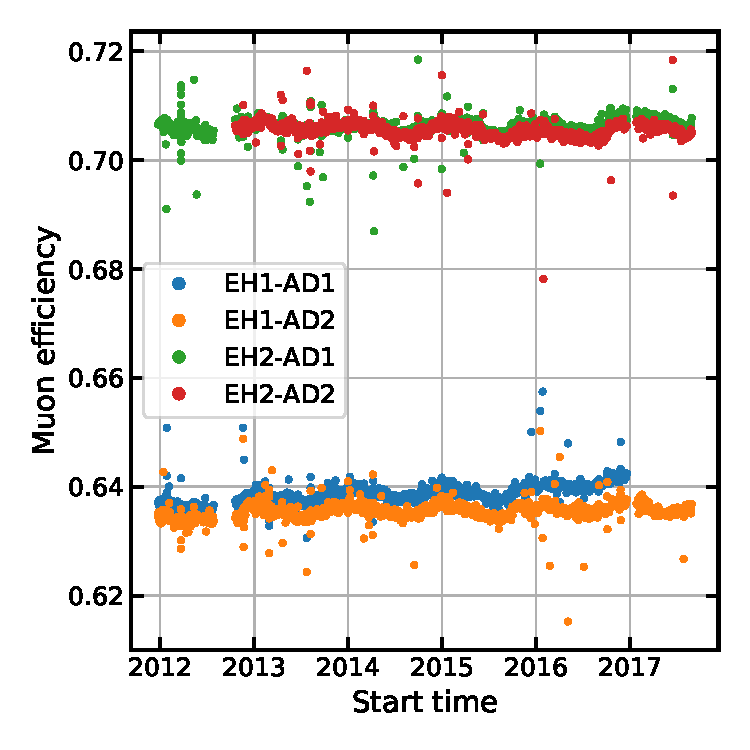
\includegraphics[width=0.48\textwidth]{plot_diagnostics/muon_eff_near_bydate}
    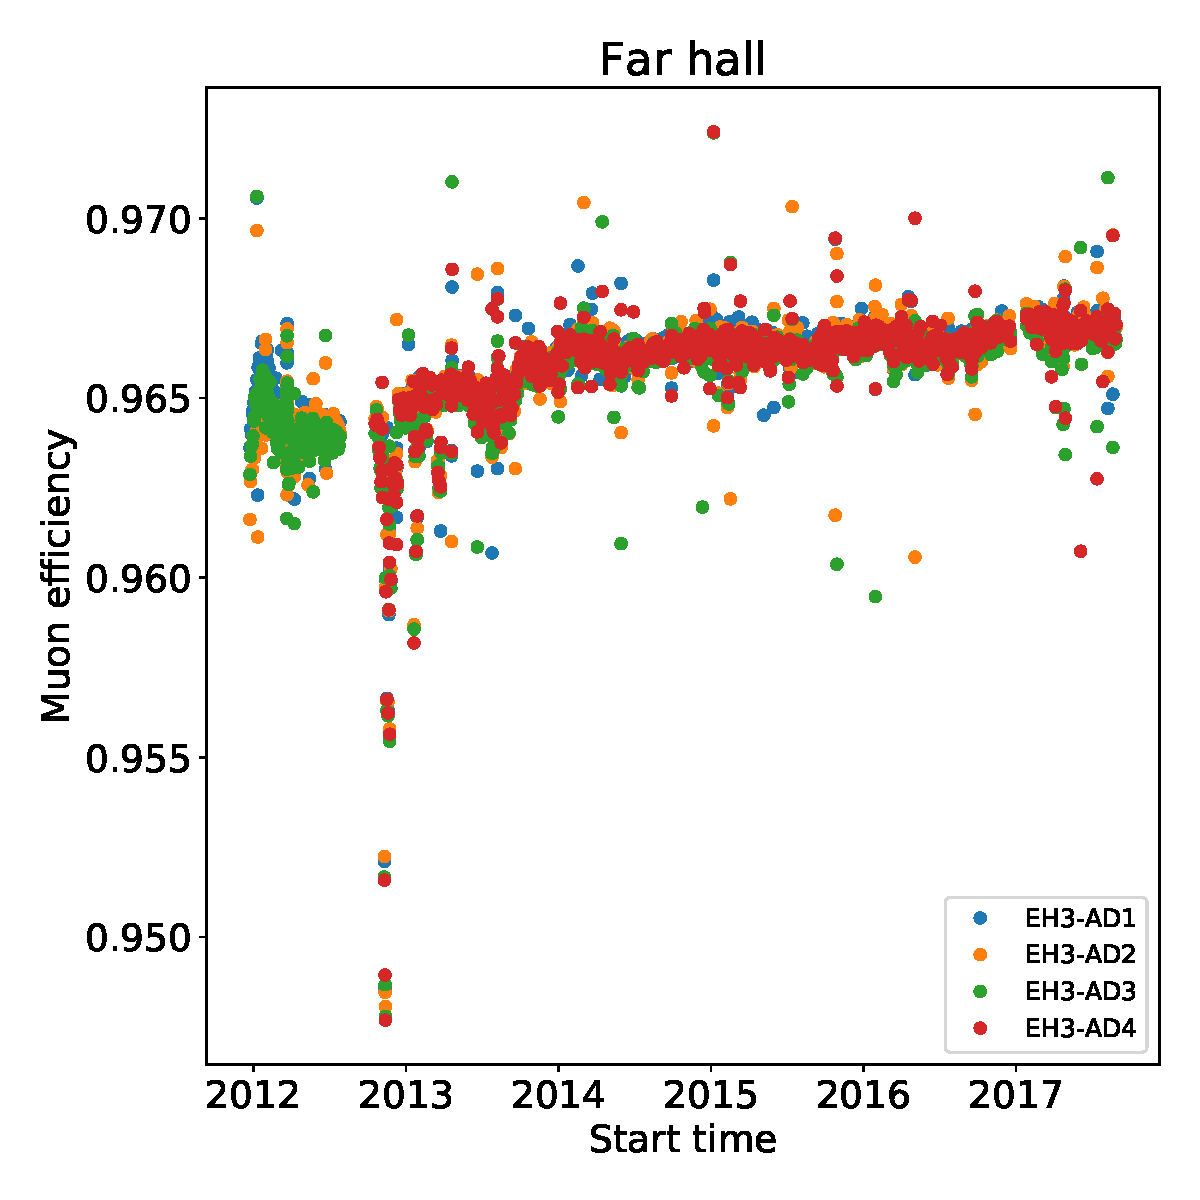
\includegraphics[width=0.48\textwidth]{plot_diagnostics/muon_eff_far_bydate}
    \caption[Muon veto efficiency over time]{
        Muon veto efficiency $\varepsilon_\mu$ over time for
        the near halls (left) and far hall (right).
        Each data point represents one data run.
        The elevated rate in EH3 is explained in the text.
    }
    \label{fig:veto_eff}
\end{figure}

\begin{figure}
    \centering
    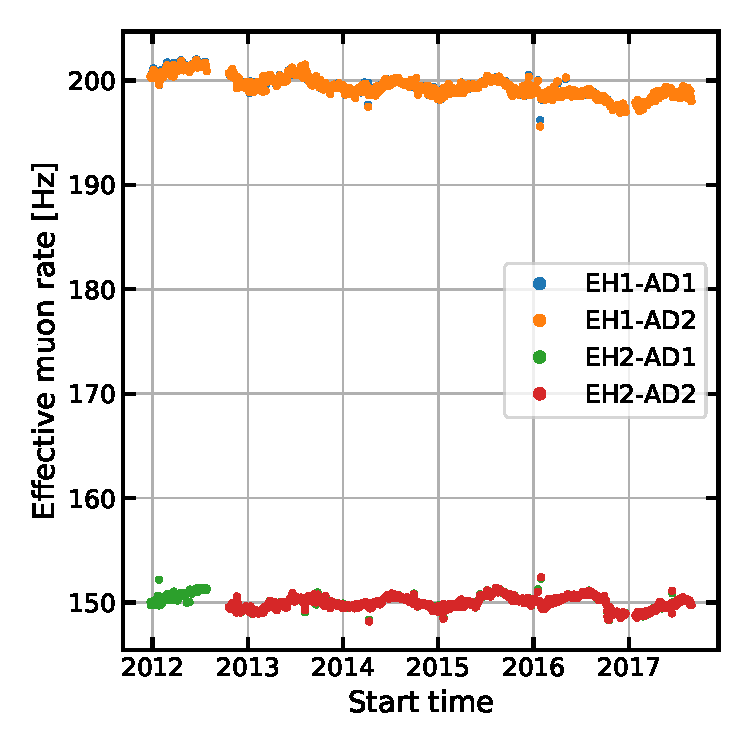
\includegraphics[width=0.48\textwidth]{plot_diagnostics/muon_rate_near_bydate}
    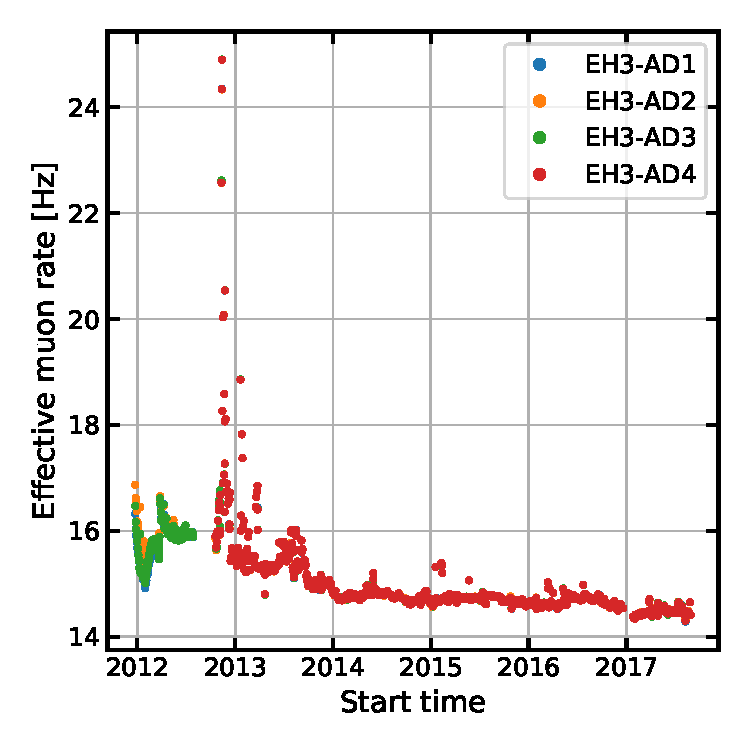
\includegraphics[width=0.48\textwidth]{plot_diagnostics/muon_rate_far_bydate}
    \caption[Effective muon rate over time]{
        Effective muon rate $R_\mu$ over time for the near halls and far hall.
        Each data point represents one data run.
        ADs in the same hall have nearly identical muon rates.
        The elevated rate in EH3 is explained in the text.
    }
    \label{fig:muon_rate}
\end{figure}

The muon veto also affected the coincidence selection
described in \cref{sec:coincidence}.
Briefly, if a candidate prompt event was followed
by both a candidate delayed event and a muon event,
then the coincidence pair was rejected as being too close to a muon event.
This avoided an unwanted correlation between muon rate
and coincidence distance-time (DT) efficiency (\cref{sec:DT_cut}).
Because of this implicit pre-muon veto window,
for a given coincidence time cut \tc,
an isolated water shield muon actually vetoed $\SI{400}{\micro\second}+\tc$
of DAQ live time,
an AD muon vetoed $\SI{800}{\micro\second}+\tc$,
and a showering muon vetoed $\SI{1}{\second}+\tc$
(\SI{1900}{\us}, \SI{2300}{\us}, and \SI{1.0015}{\s}, respectively,
for $\tc=\SI{1500}{\us}$).

When performing the coincidence selection, no events which were vetoed by muons
were considered.
Therefore, the measured rate of IBD events
must be corrected by an efficiency $\varepsilon_\mu$
accounting for the IBD events which were rejected along with the muon veto.
$\varepsilon_\mu$ is simply the fraction of DAQ time
that was not vetoed by any muon veto windows (including the pre-muon veto).
It was computed for each run as
\begin{equation}\label{eq:muon_eff}
    \varepsilon_\mu = \frac{\sum_i \Delta t_i}{t_{\text{DAQ}}},
\end{equation}
where $t_{\text{DAQ}}$ is the total time
between the first and last event in a run,
$i$ runs over all time intervals \textit{not} vetoed by a muon,
and $\Delta t_i$ is the length of interval $i$.
$\varepsilon_\mu$ should not be confused
with the fraction of muons which were identified by the muon criteria,
which is \SI{100}{\percent} \cite{muonsystem2015}.
The muon veto efficiency over time for the near and far halls
is shown in \cref{fig:veto_eff} for each data run.
The decrease in $\varepsilon_\mu$ in EH3 in late 2012 and early 2013
was caused by a so-called ``hot channel'' PMT (that may also have
emitted light due to electrostatic discharge sparks)
causing additional triggers in the water shield system
even when there were no actual muons present.
The only impact on the quality of data was additional unnecessary veto windows
causing the loss of a small amount of data.

The effective muon rate $R_\mu$ was computed for each run
by counting the number of muon veto windows
after combining overlapping windows, and dividing by the muon-corrected
livetime $\varepsilon_\mu t_{\text{DAQ}}$.
Overlapping windows were combined and counted as a single ``muon event.''
This effective quantity was useful
because when computing the counting statistics of single and coincident events
(\cref{sec:acc}),
the relevant metrics are the time until the next veto window begins
and the time since the last veto window ended,
neither of which depends on the length of a veto window
or the number of overlapping muon vetos.
The following scenarios could lead to overlapping muon veto windows:
\begin{itemize}
    \item A single physical muon could create multiple muon events
        that satisfy up to three of the four muon criteria,
        if that muon created signals in the inner and outer water shields,
        and also entered an AD and deposits at least \SI{20}{\mev} worth of scintillation light.
        Such a muon would be an inner water shield muon,
        an outer water shield muon, and an AD
        (or showering) muon.
    \item Multiple muons could randomly occur in quick succession,
        such that the second muon occurred within the veto window of the first.
    \item One muon could occur shortly after the end of a previous veto window,
        so that the pre-muon veto of the later muon overlapped with the
        post-muon veto of the earlier one.
        Any candidate event occuring between the two muons would be vetoed.
\end{itemize}
The run-by-run effective muon rate $R_\mu$ is shown in \cref{fig:muon_rate}.


%\section{Initial data preparation}
%\label{sec:dataprep}

%Before physics events are identified,
%major backgrounds that can be cleanly rejected are identified and removed.
%First, events with trigger types not used for the \thetaot{} analysis
%are discarded (see \cref{tab:trigger}).
%This includes random triggers, RPC triggers, and cross triggers.
%Second, cosmogenic muon events are identified
%and a time window after each muon is vetoed
%to allow for any spallation products or activated nuclei to decay
%without contaminating the IBD signal.
%\begin{itemize}
    %\item An IWS event with \num{>12} hit PMTs or an OWS event with \num{>15} hit PMTs
        %is considered a water shield muon.
        %All events in the subsequent \SI{400}{\us} are vetoed.
    %\item An AD event with $E > \SI{20}{\MeV}$ is considered an AD muon.
        %All events in the subsequent \SI{800}{\us} are vetoed.
    %\item An AD event with $E > \SI{2500}{\MeV}$ is considered a showering muon.
        %These muons have created particle showers within the AD,
        %and therefore have a higher probability of creating the activated nuclei
        %\isotope[9]{Li}, \isotope[8]{He}, or \isotope[12]{B}.
        %They occur infrequently enough that
        %all events in the subsequent \SI{1}{\s} can be vetoed
        %without a substantial decrease in livetime efficiency.
%\end{itemize}
%The full details of the muon veto are presented in \cref{sec:muonveto}.

%Next, occurrences of PMT light emission, known as ``flashers,''
%are also vetoed and removed from the data stream.
%These events are caused by sparking in the dynode of the PMT
%and have a geometrical signature in the pattern of hit PMTs.
%The flasher PMT itself observes a high amount of charge,
%as do the PMTs on the opposite wall of the AD,
%due to the directional emission of light from the flasher PMT.
%A cut based on the charge pattern is used to reject flashers
%with a negligible inefficiency for true IBDs.
%The details of the flasher cut are described in \cref{subsec:flashers}.

%Lastly, the vast majority of naturally-occuring radioactivity is rejected
%using an initial energy cut of \SI{1.5}{\MeV}.
%Since the oscillation minumum for Daya Bay occurs at $\sim\SI{3}{\MeV}$,
%this cut preserves the information needed for oscillation measurements.
%Even with low-energy events vetoed, a substantial number of
%uncorrelated radioactive decays are present in the final dataset
%and, when two such decays accidentally occur within a short time window,
%creat the accidental background, which will be discussed in \cref{subsec:acc}.

\section{Flasher events}
\label{sec:flashers}

\begin{figure}
    \centering
    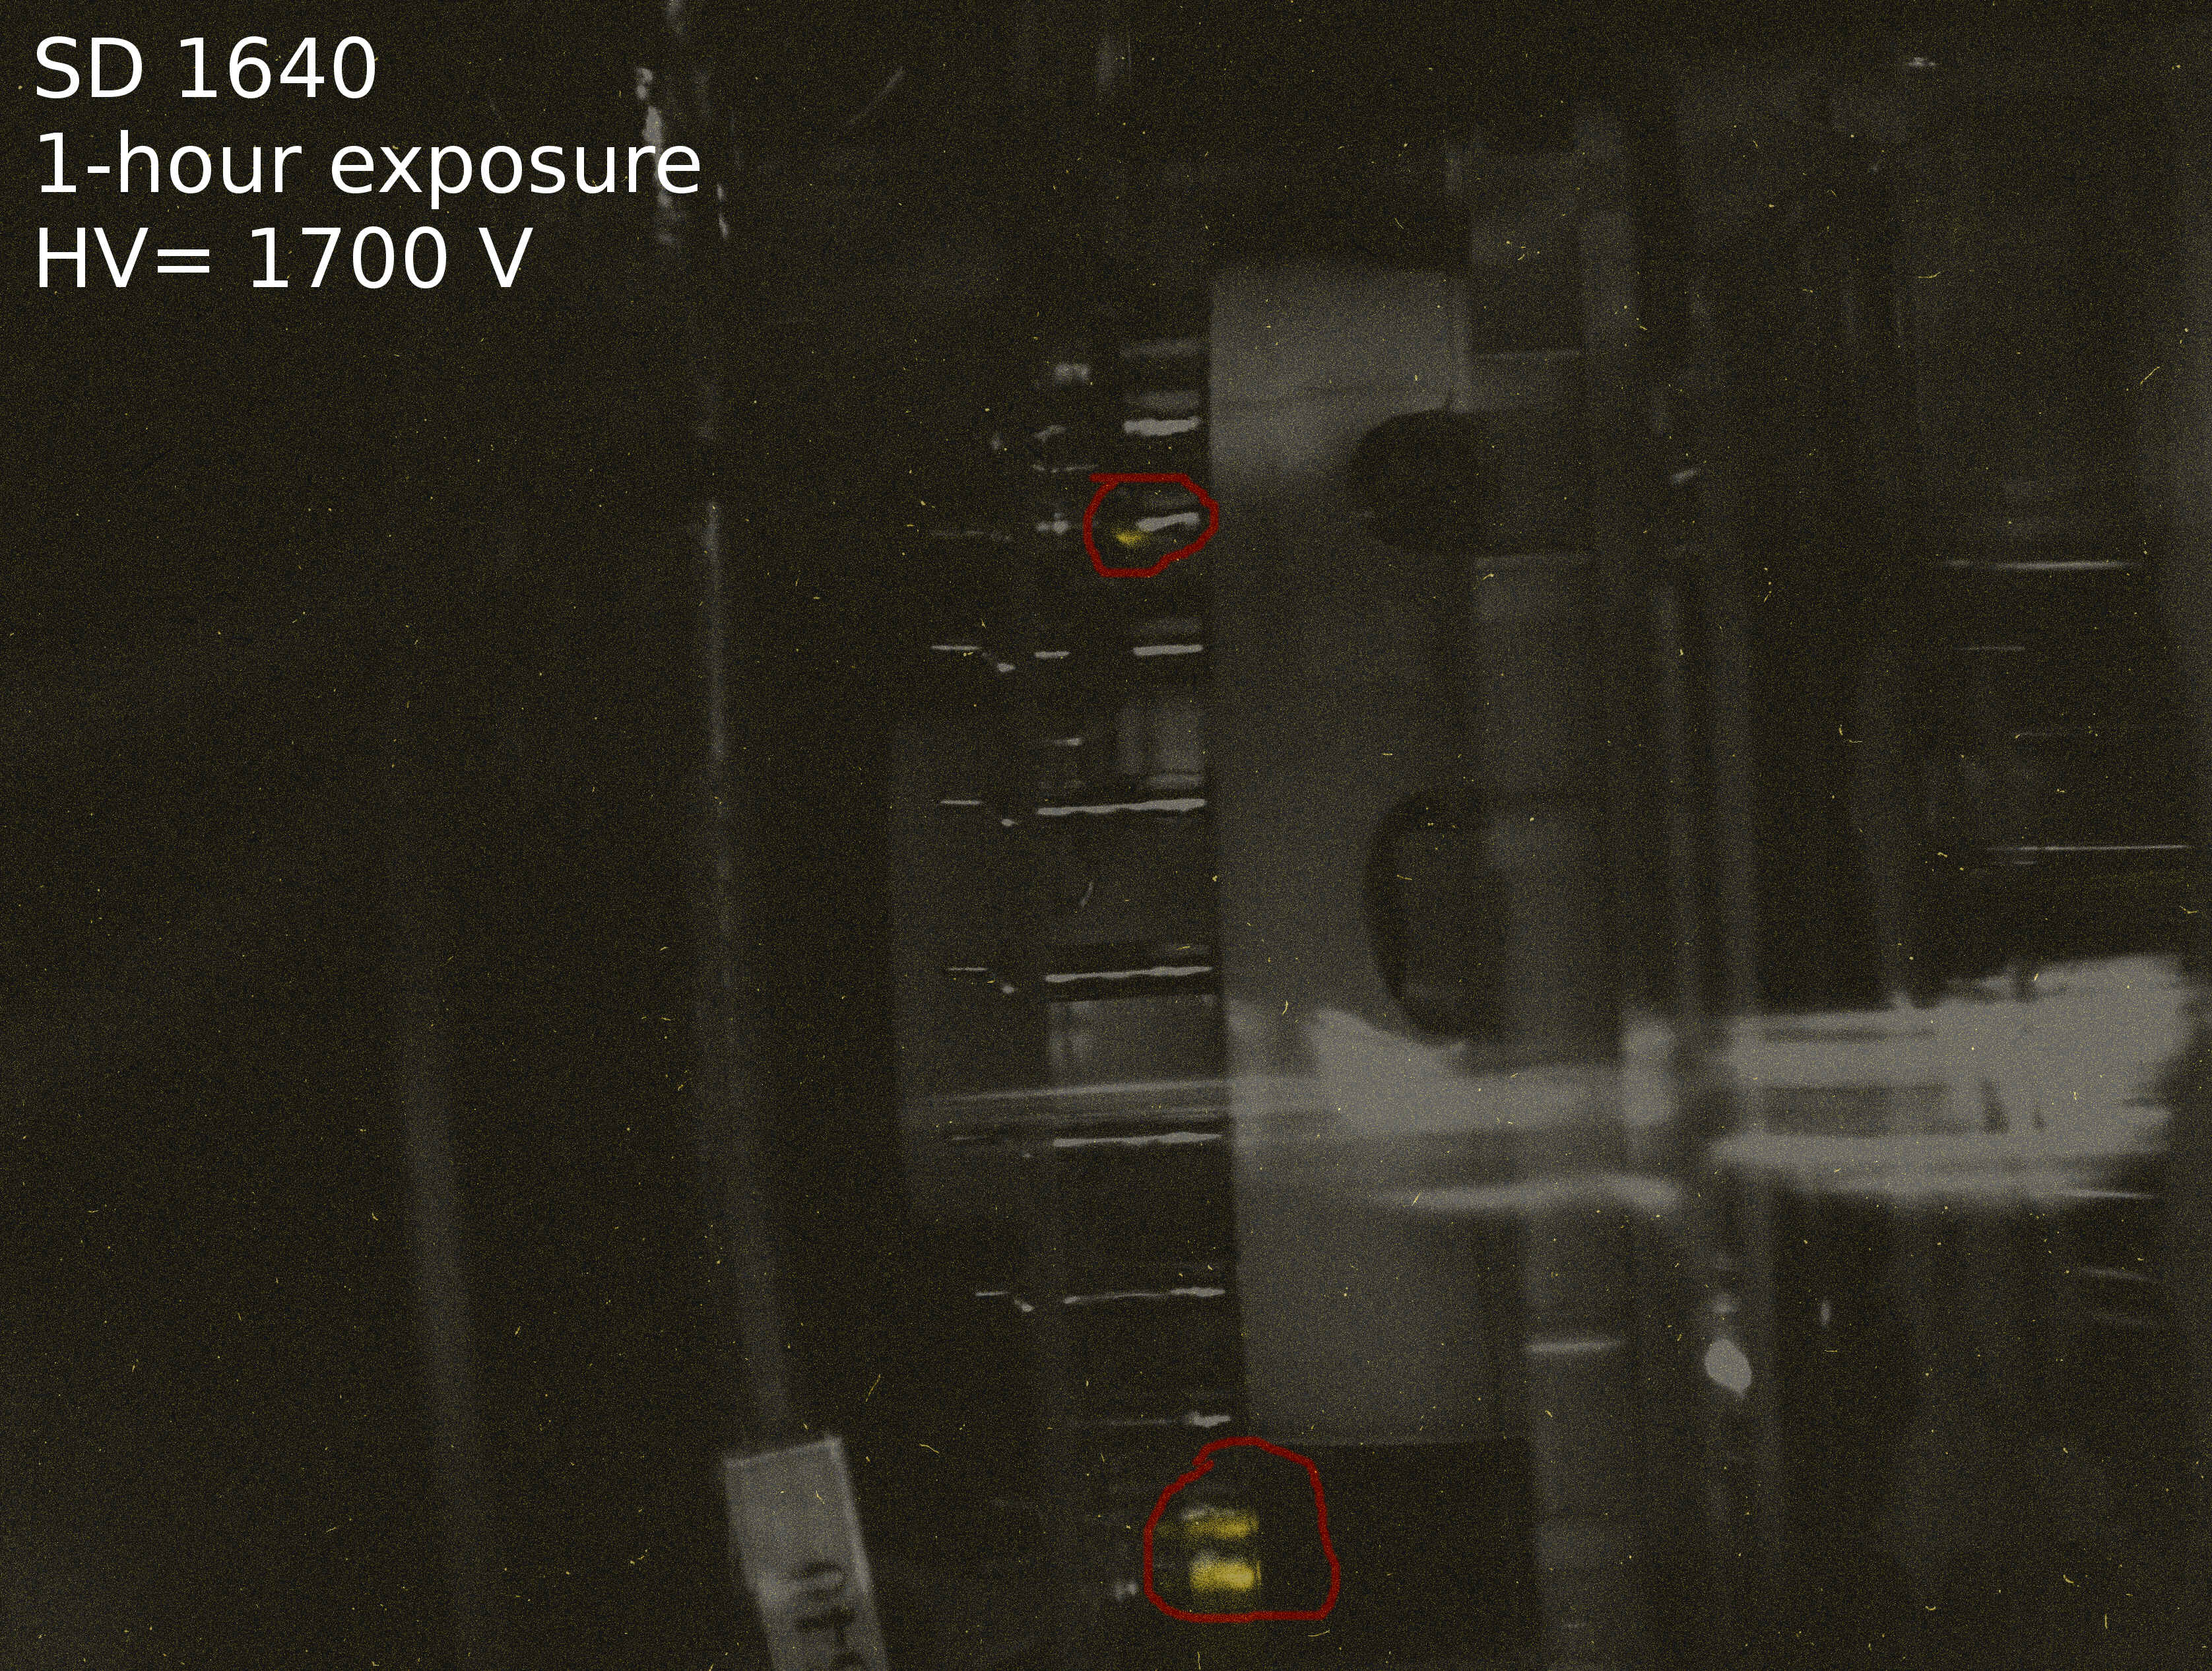
\includegraphics[width=0.8\textwidth]{ch_event_selection/flasher_photo}
    \caption[Photograph of flashing PMT]{
        Observation of electrostatic breakdown at the base of a Daya Bay PMT
        \cite{flasherphotos_docdb}.
    }
    \label{fig:flasher_photo}
\end{figure}

The high voltage required to operate PMTs rendered them susceptible
to electrostatic breakdown (sparks), also known as flashing.
In the Daya Bay PMTs, flashing was observed
at the PMT base circuit board (\cref{fig:flasher_photo}) \cite{flasherphotos_docdb}.
Although the PMT bases were isolated from the
PMT photocathodes by the black radial shield (\cref{ch:detector}),
light from the spark could propagate within the PMT
or otherwise circumvent the shielding.
These photons created signals at the PMT's own photocathode
or traversed the scintillating region and triggered other PMTs.
Five distinct signatures were observed for flasher events.
\begin{itemize}
    \item ``Nominal flashers.'' Photons activated the flashing PMT's own photocathode,
        creating a large signal.
        Other photons traversed the scintillating region and were incident
        on the PMTs directly across the AD, creating additional large signals.
        Other PMTs observed only small signals.
        Additionally, the shape of the voltage (charge) pulse from the
        flashing PMT was broader than an ordinary signal.
    \item ``2-inch flashers.'' The three 2-inch PMTs in each AD
        used to monitor the scintillator and mineral oil quality also caused flasher events.
        The signature was a large signal in one of those PMTs.
    \item ``Top-ring flashers.'' Groups of signals were observed
        with reconstructed positions far above the top ring of PMTs
        and outside the scintillating region.
        The physical origin of these flashers is not well understood,
        but one possibility is that light from a flashing PMT
        could escape the base of the PMT
        and pass through a small gap between the radial shield
        and the reflector at the top of the ADs.
        The corresponding gap at the bottom of the ADs was much smaller,
        explaining the absence of bottom-ring flashers.
    \item ``Large-$R$ flashers.'' Groups of signals were observed
        with reconstructed positions far outside the scintillating region.
        The physical origin of these flashers is not well understood.
    \item ``Cluster flashers.''
        During investigations of the other types of flasher events,
        groups of signals were observed that survived the existing cuts
        but were suspected to be flashers.
        Their physical origin is poorly understood.
\end{itemize}

Flasher events occasionally generated enough light to be categorized as muon-like events.
Events that satisfied both a muon criterion and a flasher criterion
were conservatively treated as muons.

\begin{figure}
    \centering
    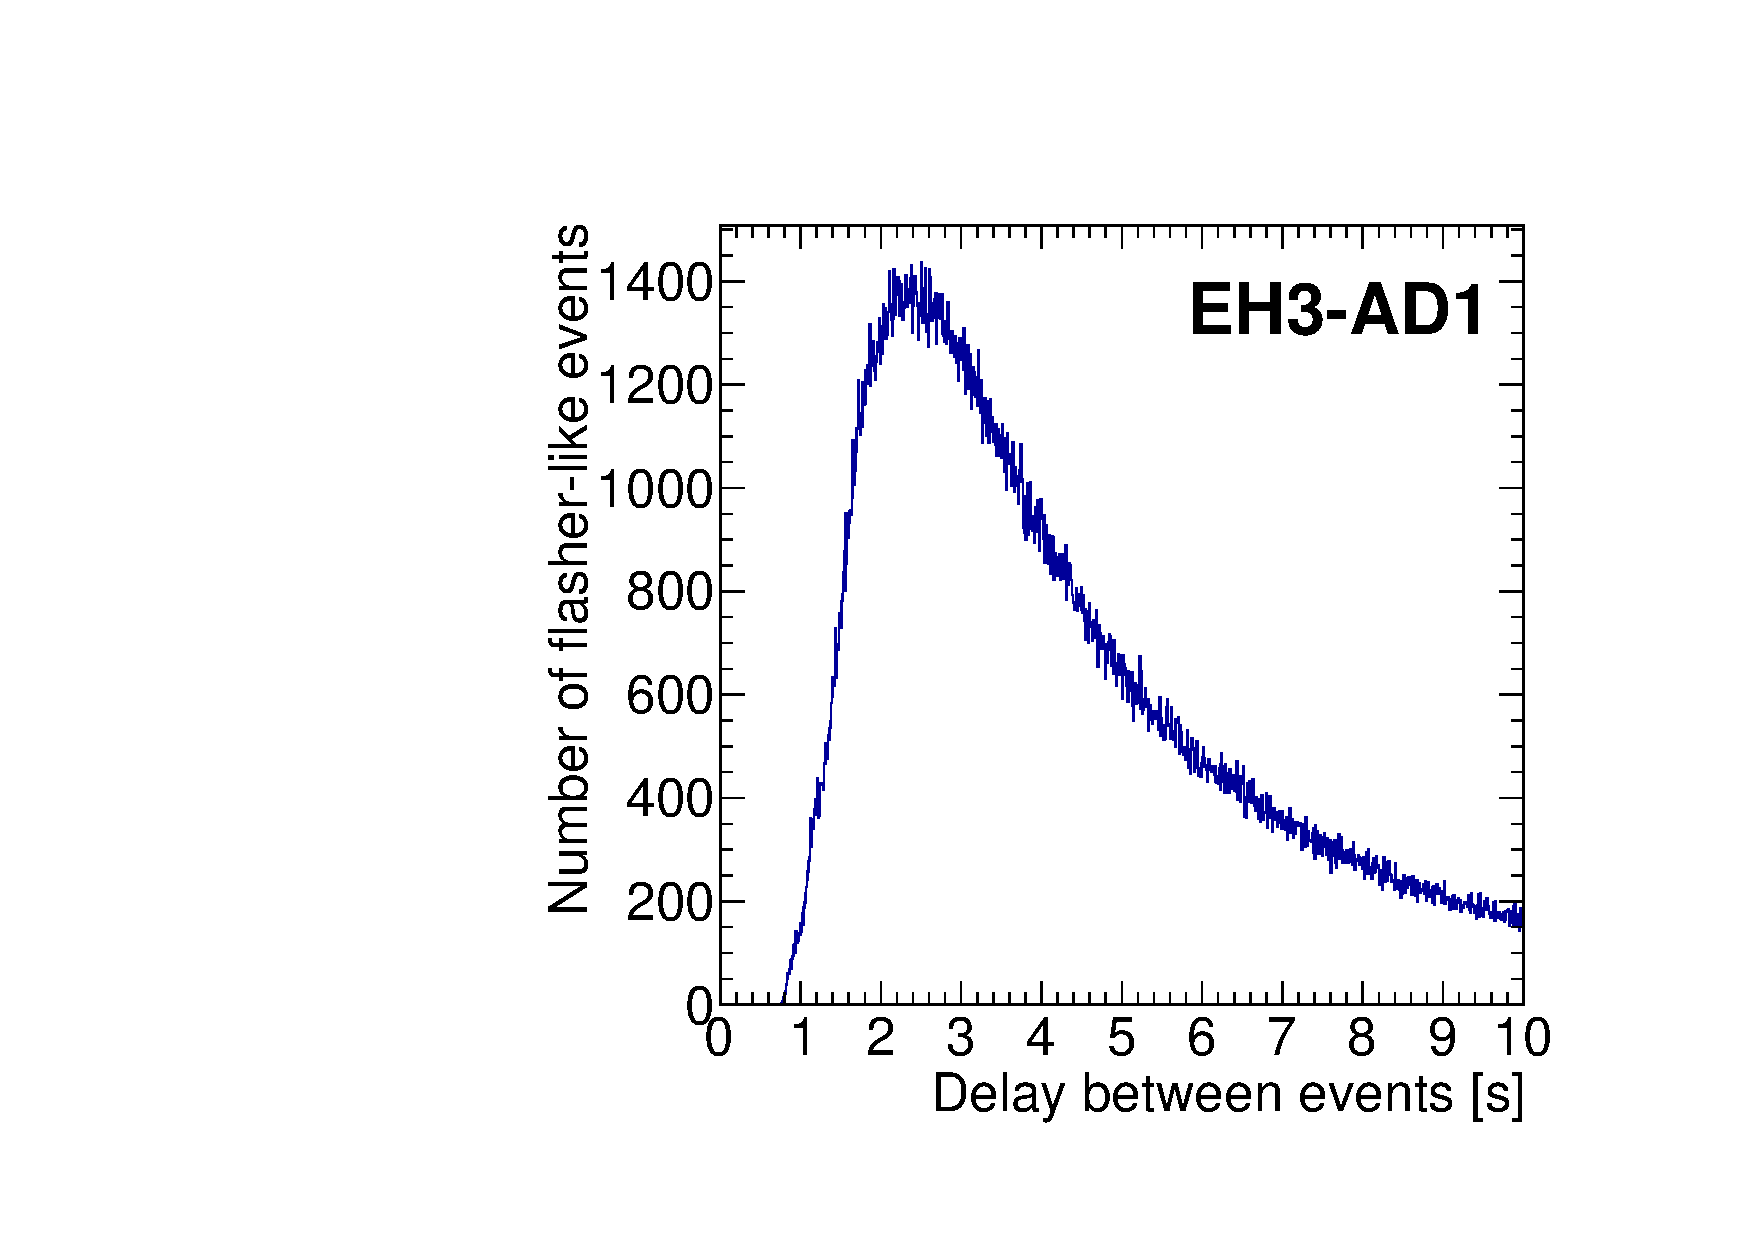
\includegraphics[width=0.48\textwidth]{ch_event_selection/resid_flasher_dt_EH3_AD1}
    \includegraphics[width=0.48\textwidth]{%
        ch_event_selection/resid_flasher_dt_zoomed_EH3_AD1%
    }
    \caption[Residual flasher $\Delta t$ distribution]{
        Left: Distribution of time delays
        of a subset of residual flashers in EH3-AD1.
        Right: The same distribution, zoomed in to shorter delays.
        The minimum coincidence time of a residual flasher pair was always
        $\gtrsim \SI{0.7}{\s}$.
        Plots taken from \cite{beda_resid_flasher_dt}.
    }
    \label{fig:flasher_anticorr}
\end{figure}


Previous Daya Bay analyses only rejected the first two types of flashers,
nominal and 2-inch flashers,
because the latter three types were accounted for
as part of the uncorrelated background (\cref{sec:acc}).
Additional efforts within the Daya Bay collaboration
to characterize the remaining so-called residual flashers
revealed that these events were not purely uncorrelated,
and so could not be fully accounted for as part of the uncorrelated background.
In particular, the distribution of time delays
between consecutive residual flashers
showed that they were anti-correlated in time:
as shown in \cref{fig:flasher_anticorr},
a residual flasher never flashed twice within $\lesssim \SI{0.7}{\s}$.
The energy distribution of the residual flasher events
limited their relevance to only the nH analysis; the nGd analysis was not affected.
The nominal and 2-inch flasher cuts are described in \cref{subsec:flash_nominal}.
The remaining flasher cuts are described in \cref{subsec:flash_resid}.

\subsection{Nominal and 2-inch flasher cuts}
\label{subsec:flash_nominal}

\begin{figure}
    \centering
    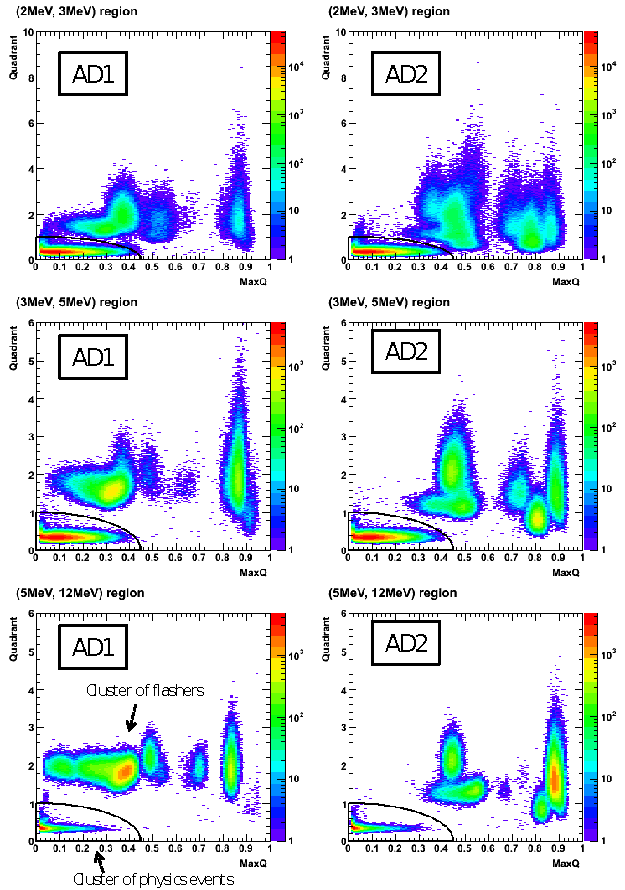
\includegraphics{ch_event_selection/nominal_flashers}
    \caption[Nominal flasher cut variables]{
        Nominal flasher cut variables for events in EH1-AD1 and EH1-AD2
        from data taken during detector commissioning in 2011.
        The ``Quadrant'' (vertical) axes show $f_\text{Quad}$,
        and the ``MaxQ'' (horizontal) axes show $f_\text{Max}$.
        The black curve in the lower-right represents $f_\text{ID} = 0$.
    }
    \label{fig:flasher_nominal_cut}
\end{figure}

The characteristic event geometry of nominal flasher events
leads to a simple discriminator to reject them on an event-by-event basis.
The flashing PMT itself had by far the largest observed charge
for a flasher event since it was the source of the emitted light.
The emitted photons traveled directly across the AD
and were incident on the PMTs opposite the flashing PMT;
PMTs which were not directly across from the flashing PMT
observed much less light.
The PMT which observed the most charge for each event
was identified as a potential flasher.
A quantity $f_{\text{max}}$ was defined as the fraction of total event charge
which was collected by the potential flasher,
$f_{\text{max}} = Q_{\text{max}}/Q_{\text{total}}$.
For nominal flasher events, $f_{\text{max}}$ was much larger than for ordinary events.
The PMTs were divided into 4 quadrants based on their column in the AD
relative to the potential flasher,
with the potential flasher at the center of Quadrant 1,
and the PMTs opposite the potential flasher assigned to Quadrant 3.
The total charge observed by the PMTs in a given Quadrant $i$
was labeled $Q_i$.
The degree to which the light in an event was focused
opposite the potential flasher
is represented by the quantity $f_{\text{quad}} = Q_3/(Q_2 + Q_4)$,
which is large when more charge is observed in Quadrant 3
relative to the two side quadrants (2 and 4).
The discriminator for nominal flashers was defined as
\begin{equation}
    f_{\text{ID}} = \log_{10}\left[
        f_{\text{Quad}}^2 + \left(
            \frac{f_{\text{max}}}{0.45}
        \right)^2
    \right],
\end{equation}
with $f_{\text{ID}} < 0$ for IBD candidates and other physics events,
and $f_{\text{ID}} > 0$ for nominal flasher events.
As shown in \cref{fig:flasher_nominal_cut},
very few events have $f_{\text{ID}}\sim0$;
it is an effective cut for unambiguously partitioning the set of events.
All nominal flasher-like events (with $f_{\text{ID}} > 0$) were rejected
and were excluded from the coincidence selection.

The 2-inch monitor PMTs also caused flasher events.
It was determined that ordinary events (non-flashers)
never deposited more than \SI{100}{\pe} worth of light
in a 2-inch PMT;
events where any 2-inch PMT observed \SI{100}{\pe} or more
were therefore rejected as 2-inch flasher events.
Additional flasher events caused by these PMTs with less than \SI{100}{\pe}
may be the physical origin of top-ring flashers,
discussed in \cref{subsec:flash_resid}.

\subsection{Residual flasher cuts}
\label{subsec:flash_resid}

\begin{figure}
    \centering
    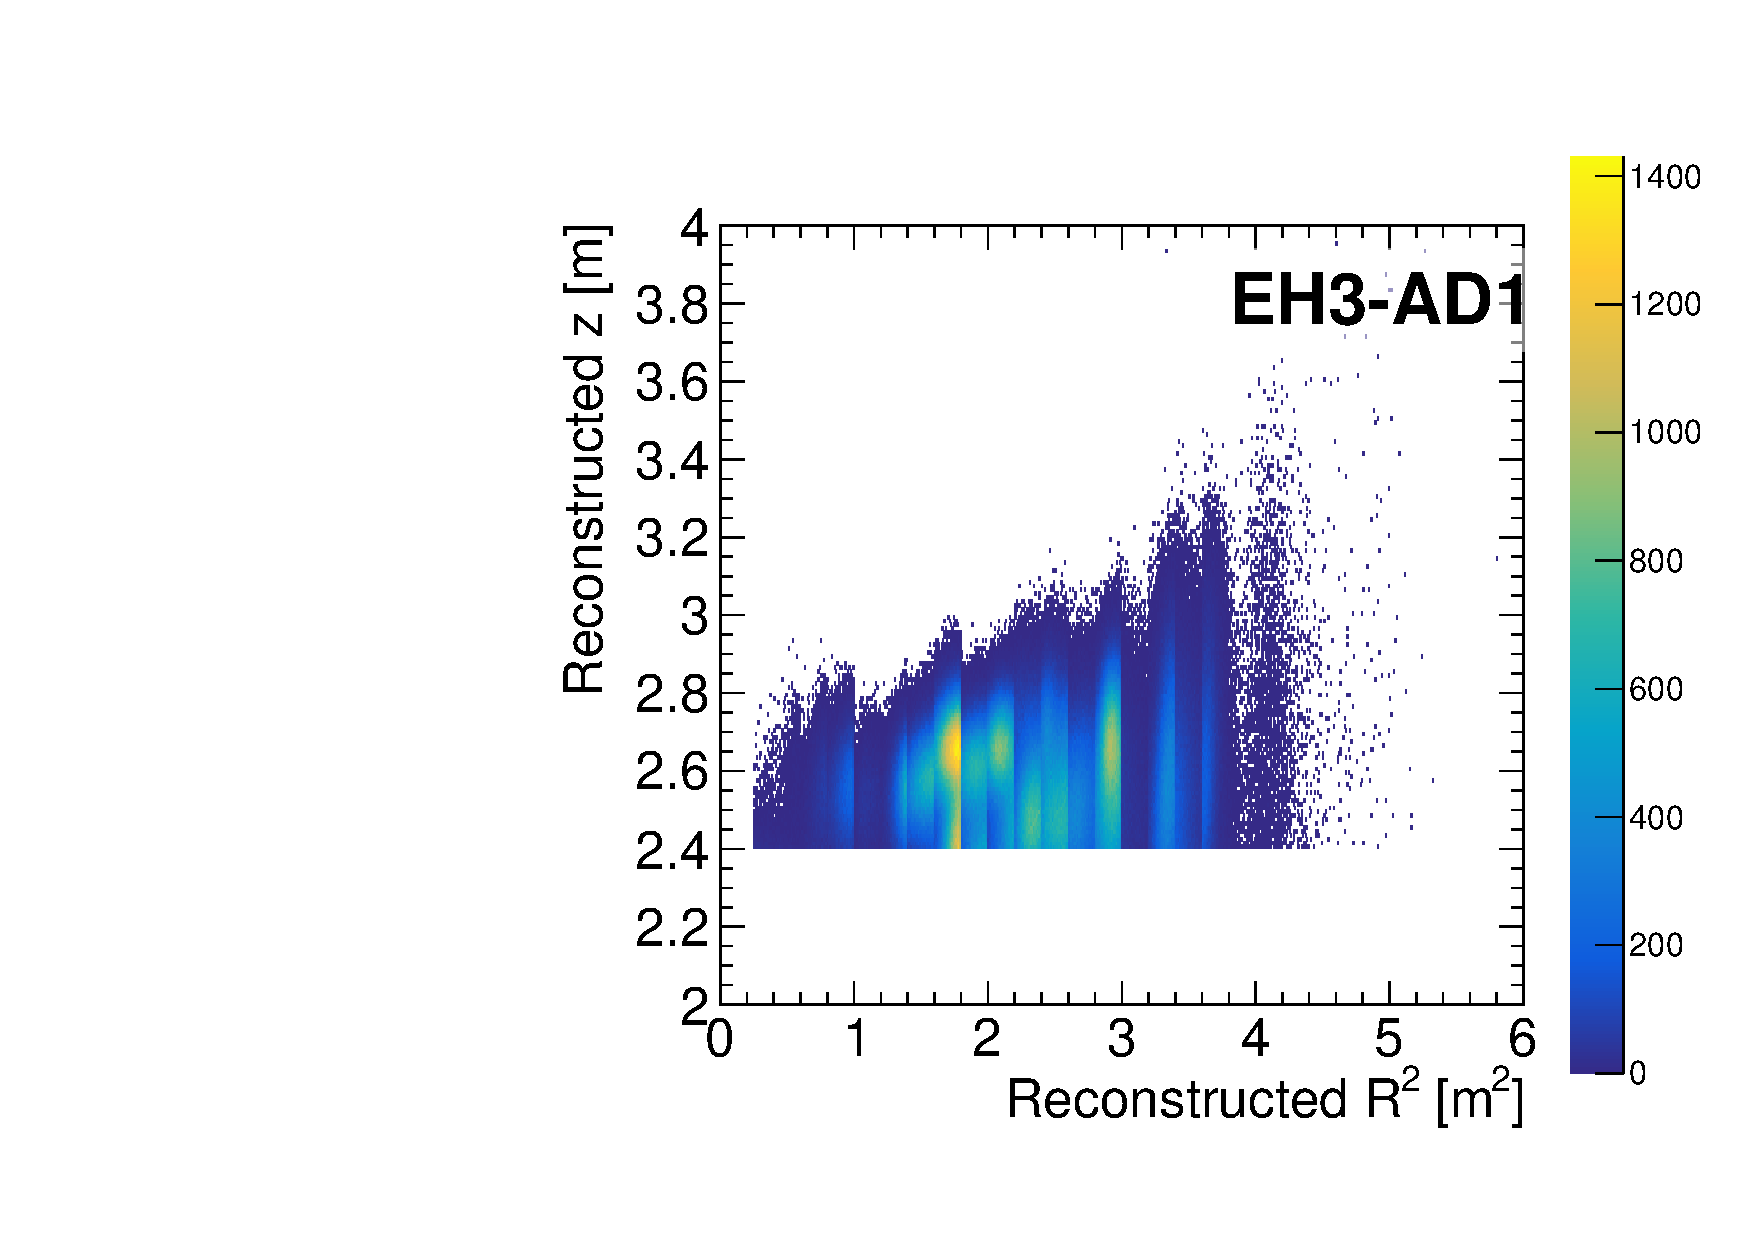
\includegraphics[width=0.49\textwidth]{ch_event_selection/flashers_top_ring_EH3_AD1}
    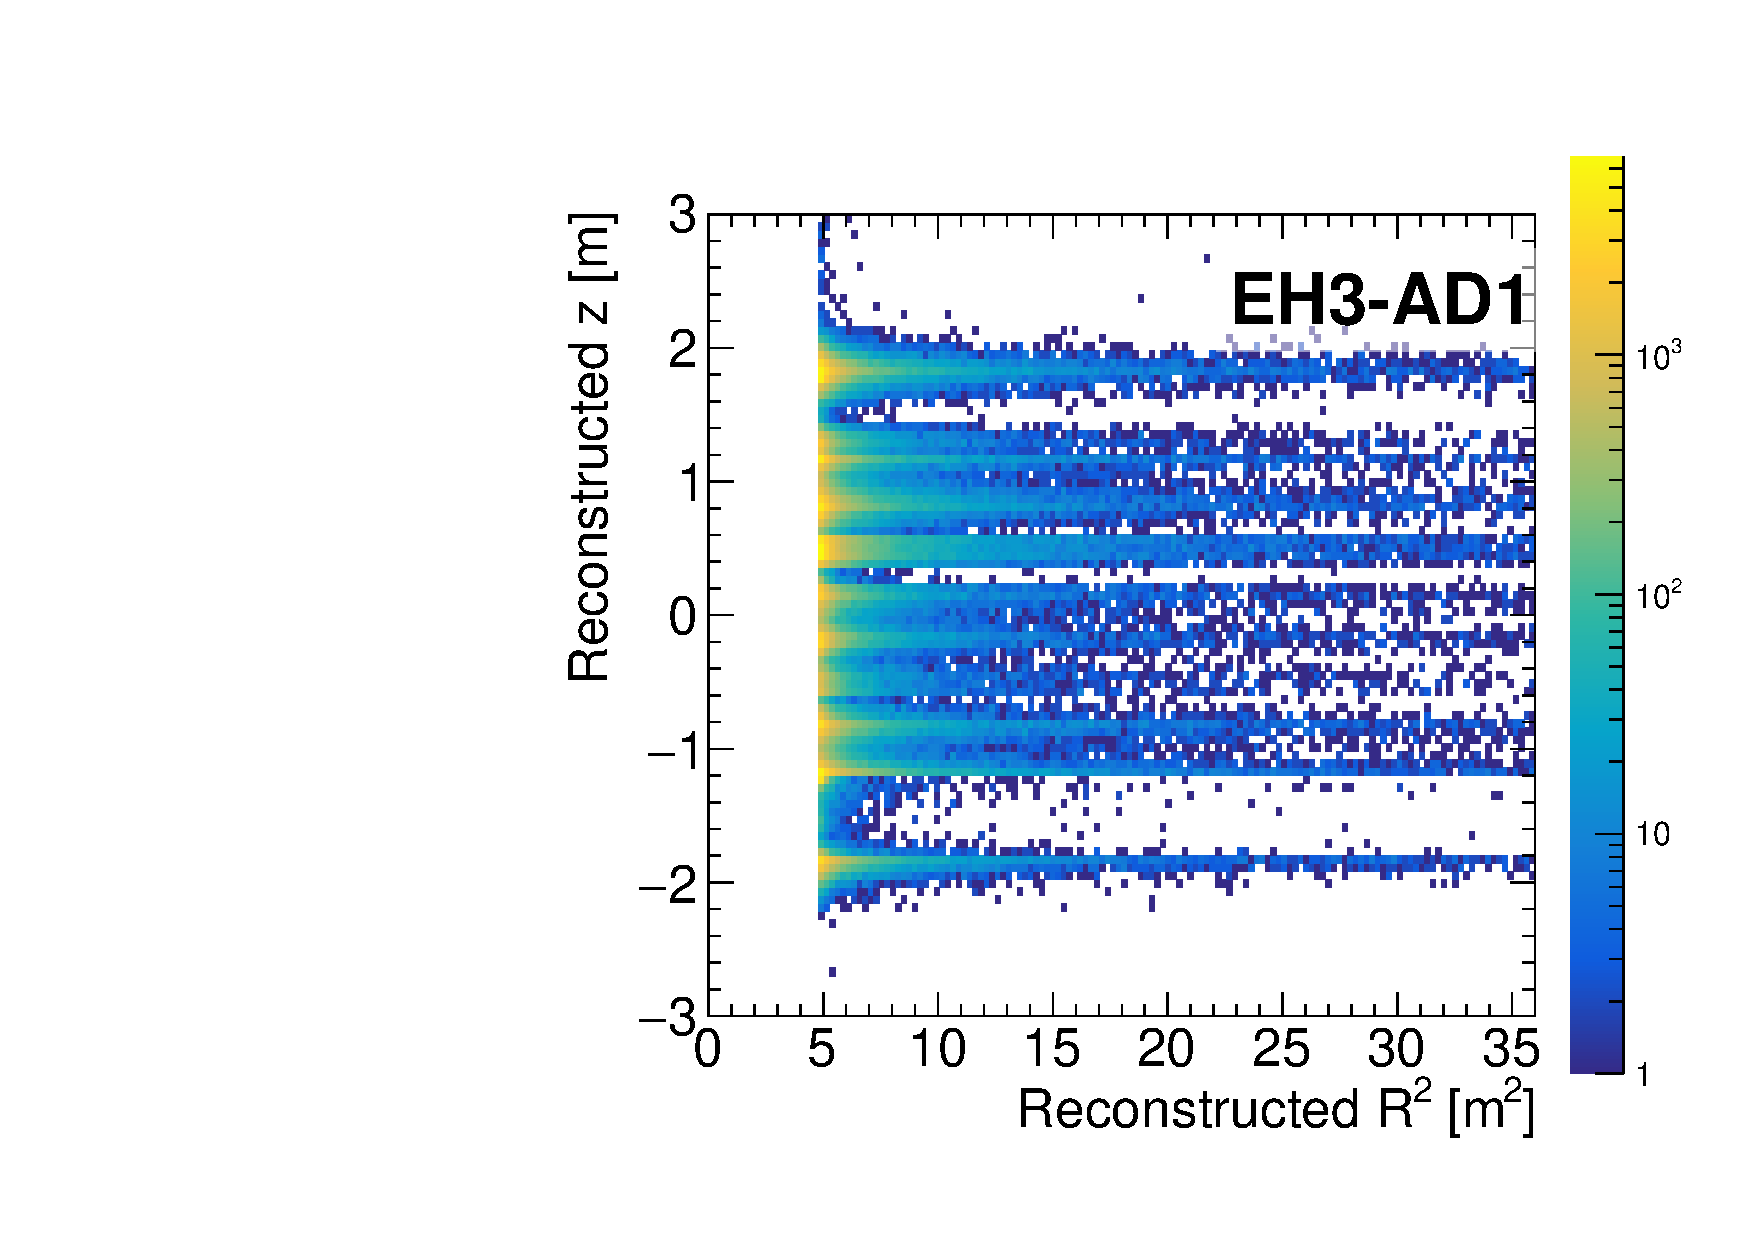
\includegraphics[width=0.49\textwidth]{ch_event_selection/flashers_outside_EH3_AD1}\\
    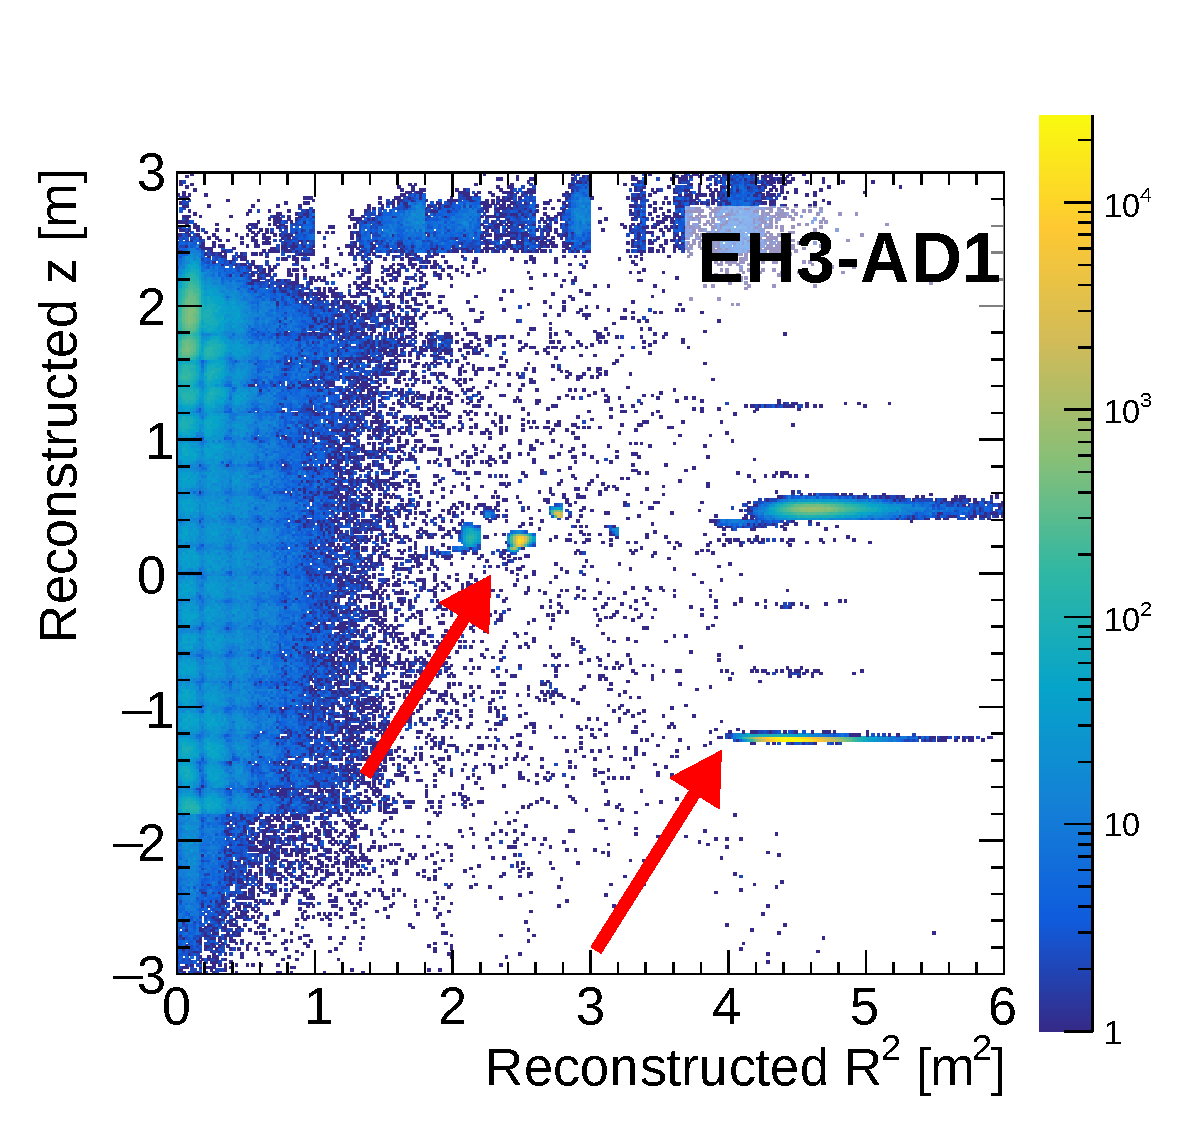
\includegraphics[width=0.5\textwidth]{ch_event_selection/flashers_hidden_EH3_AD1_arrows}
    \caption[Residual flasher position distributions]{
        Position distribution of events in EH3-AD1
        which pass the nominal and 2-inch flasher cuts,
        have $E > \SI{1.5}{\MeV}$, pass the usual muon vetos,
        and are vetoed by one of the three residual flasher cuts.
        Top left: top-ring flashers;
        top right: large-$R$ flashers;
        bottom: cluster flashers.
        The vast majority of the cluster flasher events
        within $R^2 < \SI{1}{\m\squared}$
        were isolated single events
        and thus did not impact the IBD selection efficiency.
    }
    \label{fig:flasher_resid_pos}
\end{figure}

The remaining three types of flasher events---%
top ring, large-$R$, and cluster flashers---%
were collectively referred to as residual flashers.
Their position distribution among all AD events
with energy between \SIlist{1.5;12}{\MeV}
is shown in \cref{fig:flasher_resid_pos}
Top-ring flashers were easily identified and removed
by rejecting any event with a reconstructed position
of $z > \SI{2.4}{\m}$ and $r^2 > \SI{0.25}{\m\squared}$.
(Another variant of this cut used $r^2 > \SI{0.5}{\m\squared}$.)
The number of true physical single events and
true IBD events removed by this cut was negligible.
Large-$R$ flashers were similarly easy to remove
by rejecting any event with a reconstructed position
of $r > \SI{2.2}{\m}$,
again with a negligible inefficiency for singles and IBDs.
The large-$R$ flasher cut also rejected
single events which were mis-reconstructed to have an unphysically-large radius.
These events dominate the plot showing events rejected by the large-$R$ cut.
Some of the actual large-$R$ flashers can be seen in the plot
showing the rejected cluster flasher events.

\begin{figure}
    \centering
    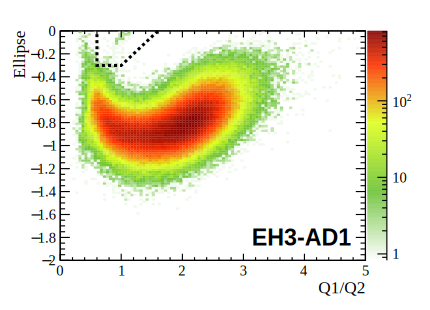
\includegraphics[width=0.6\textwidth]{ch_event_selection/hidden_flasher_post_cut}
    \caption[Cluster flasher variables]{
        Distribution of IBD candidate events in $Q_1/Q_2$-$f_{\text{ID}}$ space.
        The events within the black outline were vetoed as
        cluster flashers.
        Events above $f_{\text{ID}}=0$ were already vetoed as nominal flashers.
        The $f_\text{ID}$ parameter was also known as ``Ellipse''
        due to the shape of the cut, as is apparent in \cref{fig:flasher_nominal_cut}.
        Figure taken from \cite{flasher_plots}.
    }
    \label{fig:hidden_flasher_cut}
\end{figure}

Cluster flashers proved more difficult to isolate.
They were first noticed during an examination of the distribution of distances
between consecutive events.
Sharp peaks were observed in EH3-AD1 at distances of \SIlist{0;2.75;2.9;3.1}{\m},
and in EH3-AD3 and EH3-AD4 at \SI{0}{\m}.
Further inspection of the position distribution of events with these distances
revealed ``hot spots'' within and outside the ADs.
To isolate the cluster flashers,
various distributions were explored using the existing flasher-related variables,
including the $f_{\text{ID}}$ parameter and the various quadrant charges $Q_i$.
Eventually, a trapeziod-shaped cut in the parameter space of
$f_{\text{ID}}$ vs. $Q_1/Q_2$ was identified which rejected
$\SI{>80}{\percent}$ of hidden flashers while incorrectly rejecting only
$\SI{\sim0.02}{\percent}$ of true IBDs in each AD \cite{nh2021technote}.
Events which satisfied all of the the following three criteria were rejected:
(1) $Q_1/Q_2 > 0.6$; (2) $f_{\text{ID}} > 0.5 \times Q_1/Q_2 - 0.8$;
and (3) $f_{\text{ID}} > -0.3$,
as illustrated in \cref{fig:hidden_flasher_cut}
\cite{beda_resid_flasher_dt,flashers_jinjing}.

\section{Coincidence selection}
\label{sec:coincidence}

Events were grouped based on the number of other events
occuring within a given coincidence time \tc.
Each event with reconstructed energy above \SI{1.5}{\mega\electronvolt}
was identified as an ``AD event''
and was a potential coincidence candidate.
Because of the nonzero length of the DAQ readout window,
AD events occurring closer together than \SI{1}{\micro\second}
were not necessarily distinct physical events (see \cref{sec:daq}).
Consequently, during the coincidence grouping process,
the coincidence search windows began \SI{1}{\micro\second}
after the initial AD event.
Coincidence groups were constructed by repeating the following steps
(illustrated in \cref{fig:timeline_examples})
for all the data in a given data file \cite{thucoinc2015}:

\begin{enumerate}
    \item Find the next AD event.
        This AD event will be the ``prompt'' event of the coincidence group.
    \item Find all subsequent AD events within the desired coincidence time \tc.
        If a muon event is encountered within \tc,
        veto the entire coincidence group starting with the prompt event.
        (This additional vetoed time was accounted for in the muon veto efficiency.)
    \item Group these events together with the prompt event
        to form the coincidence group.
    \item Skip to the next AD event that is not part of the coincidence group.
\end{enumerate}

\begin{figure}
    \centering
    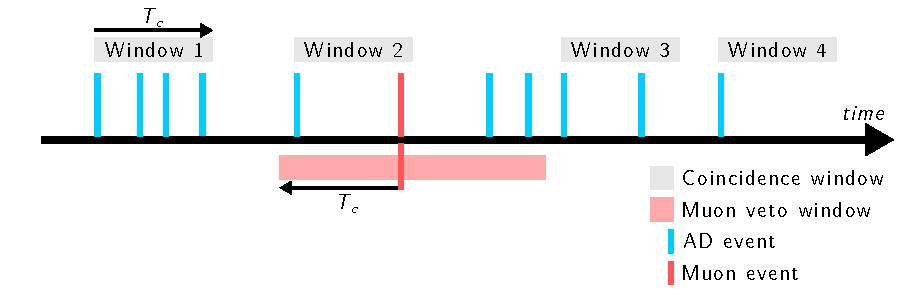
\includegraphics{ch_event_selection/timeline_examples}
    \caption[Coincidence groups diagram]{
        An example timeline showing how coincidence groups are created,
        and how they interact with muons and muon veto windows.
        This illustration does not show the \SI{1}{\micro\second} gap
        at the start of each coincidence window.
        Windows 1, 3, and 4 are valid coincidence groups,
        while Window 2 is vetoed by the muon event.
    }
    \label{fig:timeline_examples}
\end{figure}

Because of the initial \SI{1}{\micro\second} gap,
the actual time interval covered by any given coincidence window was
$\tc - \SI{1}{\micro\second}$.
This analysis uses a coincidence search window of $\tc = \SI{1.5}{\milli\second}$.

The total number of AD events in the group
is the multiplicity of the group.
A coincidence group with multiplicity $n$ is also referred to
as an \fold{n} coincidence.
In Window 1 of \cref{fig:timeline_examples},
the first AD event starts a new coincidence window
that includes three other AD events,
resulting in a coincidence group of multiplicity 4, or a \fold{4} coincidence.

If a muon event occurred within a coincidence window,
then that coincidence window was vetoed.
Therefore every muon had an implicit veto window
that excluded prompt events within \tc{} of the muon.
This is demonstrated by Window 2 of \cref{fig:timeline_examples}.
Note that if the prompt event occurred earlier than \tc{} before a muon,
then subsequent events within the coincidence window
were allowed to occur inside of the implicit muon veto window.
Only prompt events were vetoed by the implicit veto window.

The veto window after a muon also impacted the coincidence selection process.
Window 3 of \cref{fig:timeline_examples} shows a coincidence window
whose prompt event is preceded by other recent AD events.
However, those AD events fall within the previous muon veto window,
so they are ignored for the purposes of forming coincidence groups.

If a prompt event had no subsequent AD events within \tc, it was
still a valid group, and was referred to as a \fold{1} coincidence.
Note that \fold{1} coincidences are somewhat but not strictly isolated
from other AD events.
Certainly there were no other AD events
within \tc{} \textit{after} the prompt event,
but there may have been a \textit{preceding} AD event within \tc{}
if that event was part of a coincidence window
which ended before the prompt event in question.
Window 4 of \cref{fig:timeline_examples} demonstrates this property:
there are no other AD events within Window 4,
but there is a previous AD event within \tc{} of the start of Window 4.
Given the event rates at Daya Bay, this only happened in ${\sim}10^{-4}$
of single events.
This probability is derived in \cref{ap:singlesformula} as $P_b$.


\adgrid{
    All double coincidences found using $\tc=\SI{1.5}{\milli\second}$.
}{fig:double_coinc_raw}{ch_event_selection/double_coincs}{
    Prompt-delayed spectrum: all double coincidences
}

Once the coincidence groups were constructed,
the resulting set of \fold{2} coincidences
contained IBD candidates
with substantial background still present.
With a coincidence time of $\tc=\SI{1.5}{\ms}$
and a neutron capture time of $\SI{\sim200}{\us}$ in LS,
there was a negligible inefficiency due to neutrons
which took longer than \tc{} to capture on hydrogen.
\Cref{fig:double_coinc_raw} shows the prompt and delayed energy
of all \fold{2} coincidences identified each AD.
These plots clearly show the nGd events
at delayed energy values near \SI{8}{\mev}.
The nH events are visible as the narrow band with
delayed energies near \SI{2.2}{\mev}
and prompt energies of \SIrange{4}{7}{\mev}.
Above \SI{8}{\MeV}, there was a very small expected rate of IBD interactions.
Below \SI{4}{\MeV},
the nH signal events were overwhelmed by the accidental background,
which is characterized in \cref{sec:acc}.

\begin{figure}
    \centering
    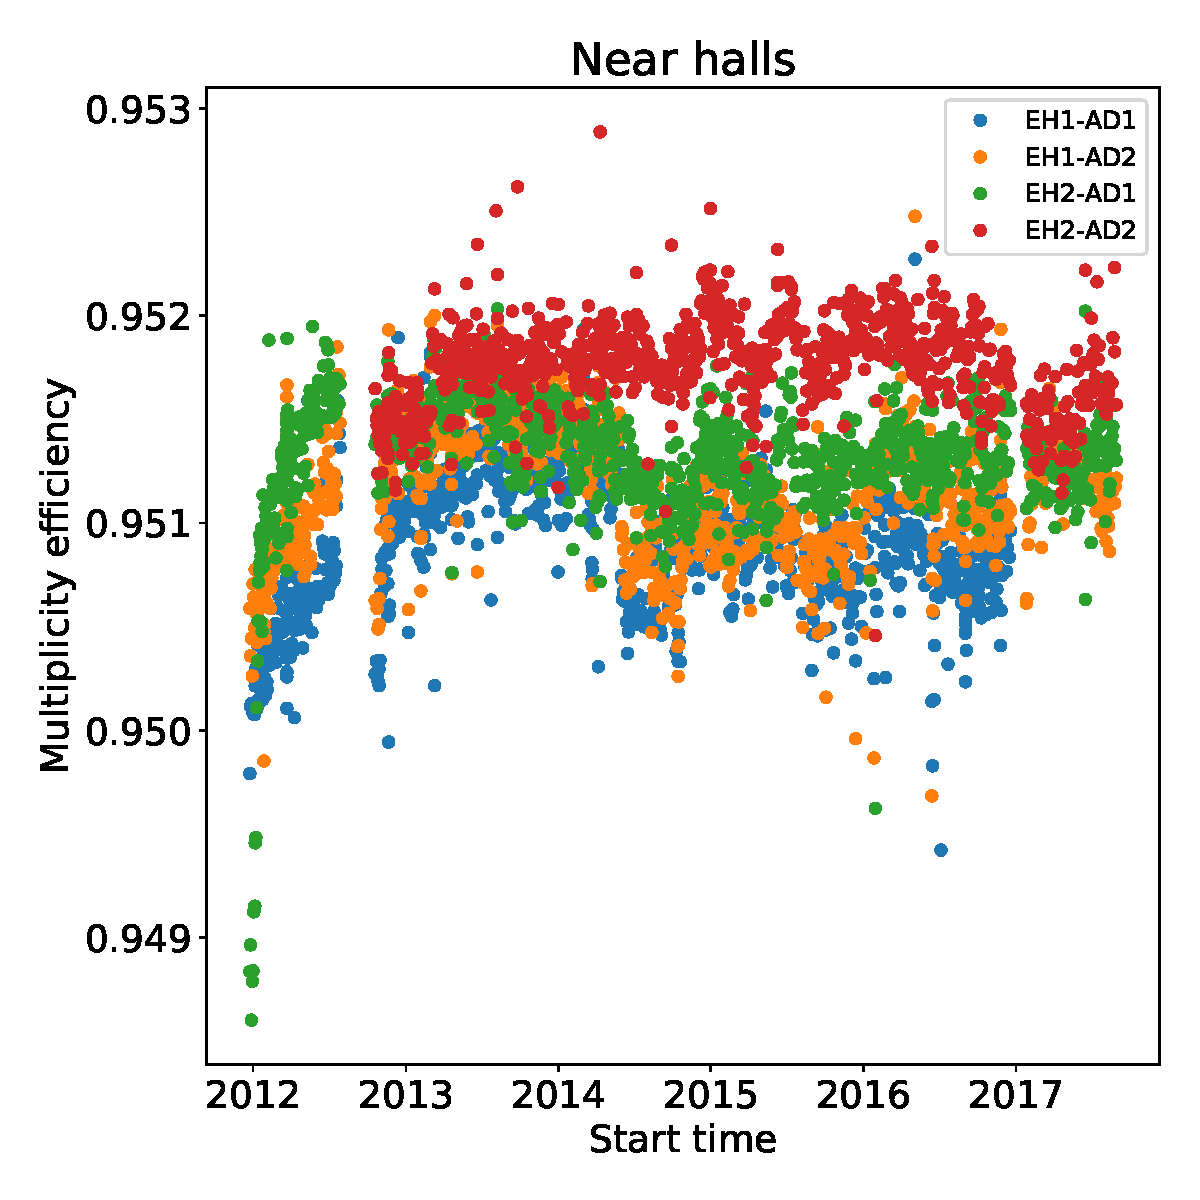
\includegraphics[width=0.48\textwidth]{plot_diagnostics/mult_eff_near_bydate}
    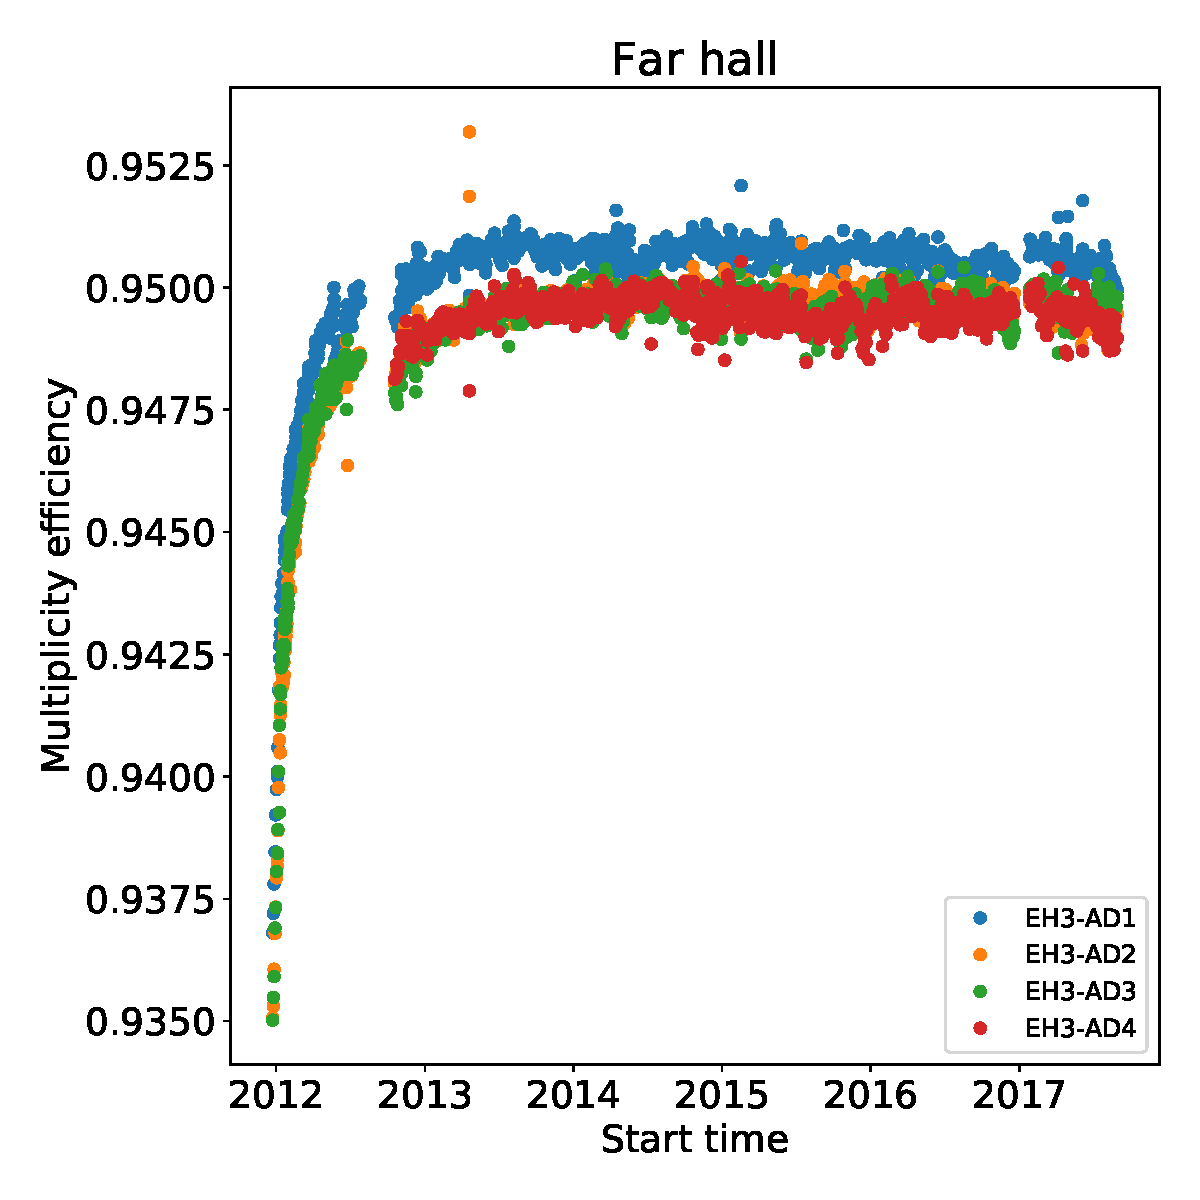
\includegraphics[width=0.48\textwidth]{plot_diagnostics/mult_eff_far_bydate}
    \caption[Multiplicity veto efficiency over time]{
        Multiplicity veto efficiency $\varepsilon_m$ over time for
        the near halls (top) and far hall (bottom).
        Each data point represents one data run.
    }
    \label{fig:mult_eff}
\end{figure}
The set of \fold{1} coincidences was a subset
of the uncorrelated events, mostly radioactive decays,
that were also present in the data stream.
However, not all uncorrelated events formed \fold{1} coincidences.
Sometimes an uncorrelated event occurred in close time proximity to
a true IBD prompt-delayed pair, creating a \fold{3} coincidence.
These high-multiplicity coincidence groups were vetoed
with a small loss of efficiency.
The efficiency of this multiplicity cut is derived in \cref{ap:singlesformula} as
\cref{eq:mult_eff_ap}:
\begin{align}
    \label{eq:mult_eff}
    \begin{split}
        \varepsilon_m &= e^{-R_s \tc}
        \left[
            e^{-(R_s + R_\mu)\tc} +
            \frac{R_s}{R_s+R_\mu} e^{-R_\mu\tc}
            \left(
                1 - e^{-(R_s + R_\mu)\tc}
            \right)
        \right. \\
              &\ \ \left. - \frac{R_s}{2R_s + R_\mu} e^{-R_\mu\tc}
                  \left(
                      1 - e^{-(2R_s + R_\mu)\tc}
                  \right) +
                  \frac{R_\mu}{R_s + R_\mu}
                  \left(
                      1 - e^{-(R_s + R_\mu)\tc}
                  \right)
              \right],
    \end{split}
\end{align}
where $R_s$ is the rate of uncorrelated events,
$R_\mu$ is the effective muon rate,
and \tc{} is the length of the coincidence window, \SI{1499}{\us}.
The multiplicity efficiency over time is shown in \cref{fig:mult_eff}.
More concerning than the multiplicity veto is when two uncorrelated events
randomly occur in close proximity to each other,
creating a \fold{2} coincidence group that passes the multiplicity veto.
These so-called ``accidental'' coincidences
constitute the largest background within the set of \fold{2} coincidences
(\cref{sec:acc}).
The distance, time and energy cuts described below
are all motivated in large part by the need to reduce the accidental background.

\section{Distance and time cuts}
\label{sec:DT_cut}

The average range of a neutron
in the Daya Bay liquid scintillator
before an nH capture
was approximately \SI{300}{\milli\meter},
and the time delay between production and capture was \SI{\sim215}{\us}.
For accidental coincidences, the typical separation between prompt and delayed signals was
the length scale of the AD, approximately \SI{4000}{\milli\meter}.
The characteristic time between consecutive single events,
based on the \fold{1} event rate of $\SI{\sim20}{\Hz}$,
was $\SI{\sim50000}{\us}$.
Thus the distance and time between the prompt and delayed signals
of a double coincidence event could be used
as discriminants to preferentially select IBD events over accidentals.

\adgrid{
    Distribution of coincidence distance and coincidence time.
}{fig:dr_vs_dt}{ch_event_selection/dr_vs_dt}{
    Coincidence distance vs. time
}

\adgrid[0.22\textheight]{
    Distribution of the DT parameter for all double coincidence events.
    The large peak consists of accidental coincidences.
    The contribution from IBDs is clearly visible
    at DT values of less than \SI{1}{\m} in EH1 and EH2.
    In EH3, the contribution from IBDs is visible
    on close inspection but is much smaller relative to the number of accidentals.
}{fig:DT_data}{ch_event_selection/DT_data}{DT parameter distribution}

\Cref{fig:dr_vs_dt} shows the distribution of
coincidence distance and coincidence time
for the subset of \fold{2} coincidences with
relatively small coincidence distances and times
of less than \SI{1000}{\milli\meter} and \SI{600}{\micro\second},
respectively.
The cluster at the lowest coincidence time and distance
consists of IBD events.
The rest of the events distributed with relatively uniform density
across the plot are accidental coincidences from uncorrelated events.
This plot was used as a heuristic to determine a distance and time cut
by drawing a line from \SI{800}{\milli\meter} at $0$ time
to \SI{480}{\micro\second} at $0$ distance.
This line separated the higher-density region
of correlated events from the uniform density region of accidental background.
The distance-time (DT) cut was defined by this line,
and accepted events that satisfied the inequality
\begin{equation}\label{eq:DT}
    \text{DT} = \Delta r + v_0 \Delta t < \SI{800}{\milli\meter},
\end{equation}
where $v_0 = \frac{\SI{1000}{\milli\meter}}{\SI{600}{\micro\second}}$.
The DT parameter distribution for the double coincidence events
in each AD is shown in \cref{fig:DT_data}.
The figure makes clear that applying a DT cut of \SI{800}{\mm}
would reject the vast majority of accidental coincidences
with what appears to be a tolerable inefficiency in IBDs.
The actual inefficiency is discussed in \cref{subsec:eff_DT}.
\Cref{fig:after_DT_cut} shows the individual AD spectra
after applying the DT cut.
As expected, the accidental background present
in the low-prompt-energy and low-delayed-energy corner was reduced.
The nH capture events now stand out much better
against the accidental background.
\adgrid{
    Prompt-delayed energy spectra after applying the DT cut
}{fig:after_DT_cut}{ch_event_selection/post_DT_cut}{
    Prompt-delayed spectrum: after DT cut
}

\section{Prompt energy}
\label{subsec:prompt_energy}
The prompt energy lower bound of \SI{1.5}{\mev}
was chosen to exclude a substantial fraction
of the low-energy uncorrelated events from radioactive decays.
In particular, the electron capture process
${}^{40}\text{K} \to {}^{40}\text{Ar} + \nu_e + \gamma$
released a $\gamma$-ray with energy \SI{1.46}{\mev}.
Despite the \SI{1.5}{\MeV} cut,
the high-energy tail of this interaction is nevertheless visible in the prompt-delayed spectra
(\cref{fig:double_coinc_raw}) as an elevated bin content
along both the horizontal and vertical axes from \SIrange{1.5}{3}{\mev}.
An upper bound of \SI{12}{\MeV} was used for the prompt energy.
The reactor \nuebar{} spectrum falls steeply above \SI{8}{\mev}
(see \cref{fig:reactor_flux_xsec})
so this cut accepted higher-energy IBDs with negligible inefficiency.


\section{Irreducible uncorrelated background}
\label{sec:acc}

Once muon events and flashers were removed from the data stream,
the vast majority of the remaining AD events were caused by uncorrelated
natural radioactive decays and are commonly known as ``singles,''
although as will be shown shortly, this name is misleading,
and a more appropriate name is ``uncorrelated events.''
These events occurred at approximately \SI{17.5}{\hertz} in each AD
(for energies above \SI{1.5}{\MeV})
and,
because they were uncorrelated, their groupings in time followed Poisson statistics.
In particular, there was a nonzero probability that
two of these uncorrelated ``single'' events would occur within
$\tc=\SI{1.5}{\milli\second}$ and thus form a \fold{2} coincidence.
For any given uncorrelated event, the probability that
another uncorrelated event would occur within \tc{} was
\begin{equation}
    \text{Poisson}(1\vert R_s\tc) = R_s\tc e^{-R_s\tc}.
\end{equation}
For the above value for $R_s=\SI{17.5}{\hertz}$, this probability is \SI{2.56}{\percent}.
Since \fold{2} coincidence groups like this were not formed from any
deliberate physical proccess but rather by an accidental coincidence,
they are known as the accidental background.
Crucially, though all \fold{1} coincidence groups
were assumed to consist of a single uncorrelated event,
not all uncorrelated events formed \fold{1} coincidences.
These so-called ``singles'' were actually not always lone events.
A back-of-the-envelope estimate of the rate of accidental coincidences gives
$\SI{17.5}{\hertz}\times\SI{2.56}{\percent}=\SI{0.45}{\hertz}$
before applying the distance-time (DT) cut (\cref{sec:DT_cut}).

Because the delayed-energy selection criteria
were derived from the accidentals-subtracted delayed energy spectrum for each AD,
the accidentals analysis will be presented first,
followed by the specification of the delayed energy cut in \cref{subsec:delayed}.
The actual implementation of the event selection
first characterized the singles and \fold{2} rates
and created the synthetic accidentals sample
(\cref{subsec:singles,subsec:2fold,subsec:synthetic}).
Then the delayed-energy cuts were extracted (\cref{subsec:delayed}),
and finally, the number of accidental coincidences
contaminating the final IBD sample was computed (\cref{subsec:acc_count}).

\subsection{Uncorrelated events}
\label{subsec:singles}

The full accidental background subtraction procedure began with identifying
the rate of uncorrelated events in the AD, again better known
as the ``singles rate,'' for each individual data run.
The singles rate was computed by first measuring the rate of
\fold{1} coincidences in each run
(with the prompt energy bound of \SIrange{1.5}{12}{\mev} from \cref{subsec:prompt_energy}).
Given $R_\text{\fold{1}}$, the true underlying rate of uncorrelated events was
computed by numerically solving the following formula
(derived in \cref{ap:singlesformula}) for $R_s$:
\begin{align}
    \label{eq:rsingles}
    \begin{split}
        R_{\text{\fold{1}}}
          &= R_s e^{-R_s\tc}
          \left[
              e^{-(R_s + R_\mu)\tc} +
              \frac{R_s}{R_s+R_\mu} e^{-R_\mu\tc}
              \left(
                  1 - e^{-(R_s + R_\mu)\tc}
              \right)
          \right. \\
          &\ \ %
          \left. - \frac{R_s}{2R_s + R_\mu} e^{-R_\mu\tc}
              \left(
                  1 - e^{-(2R_s + R_\mu)\tc}
              \right) +
              \frac{R_\mu}{R_s + R_\mu}
              \left(
                  1 - e^{-(R_s + R_\mu)\tc}
              \right)
          \right]
    \end{split}
\end{align}
In this formula, \tc{} represents the actual duration of the coincidence window,
which technically began \SI{1}{\micro\second} after each event,
meaning that a value of $\tc=\SI{1499}{\micro\second}$ was used (\cref{sec:daq}).
This formula is valid under the assumption that all
events in the data stream were truly uncorrelated in time.
Residual flashers were anti-correlated in time
but were vetoed from the data stream (\cref{sec:flashers}).
Correlated events (both IBDs and other backgrounds)
had a rate much smaller than the uncorrelated event rate
($R_{\text{corr}}/R_s \sim 10^{-3}$)
and had a negligible impact on the probability of a \fold{1} coincidence,
as validated by the Reconstructed-Data File Simulation in \cref{subsec:sim_singles}.

\begin{figure}
    \centering
    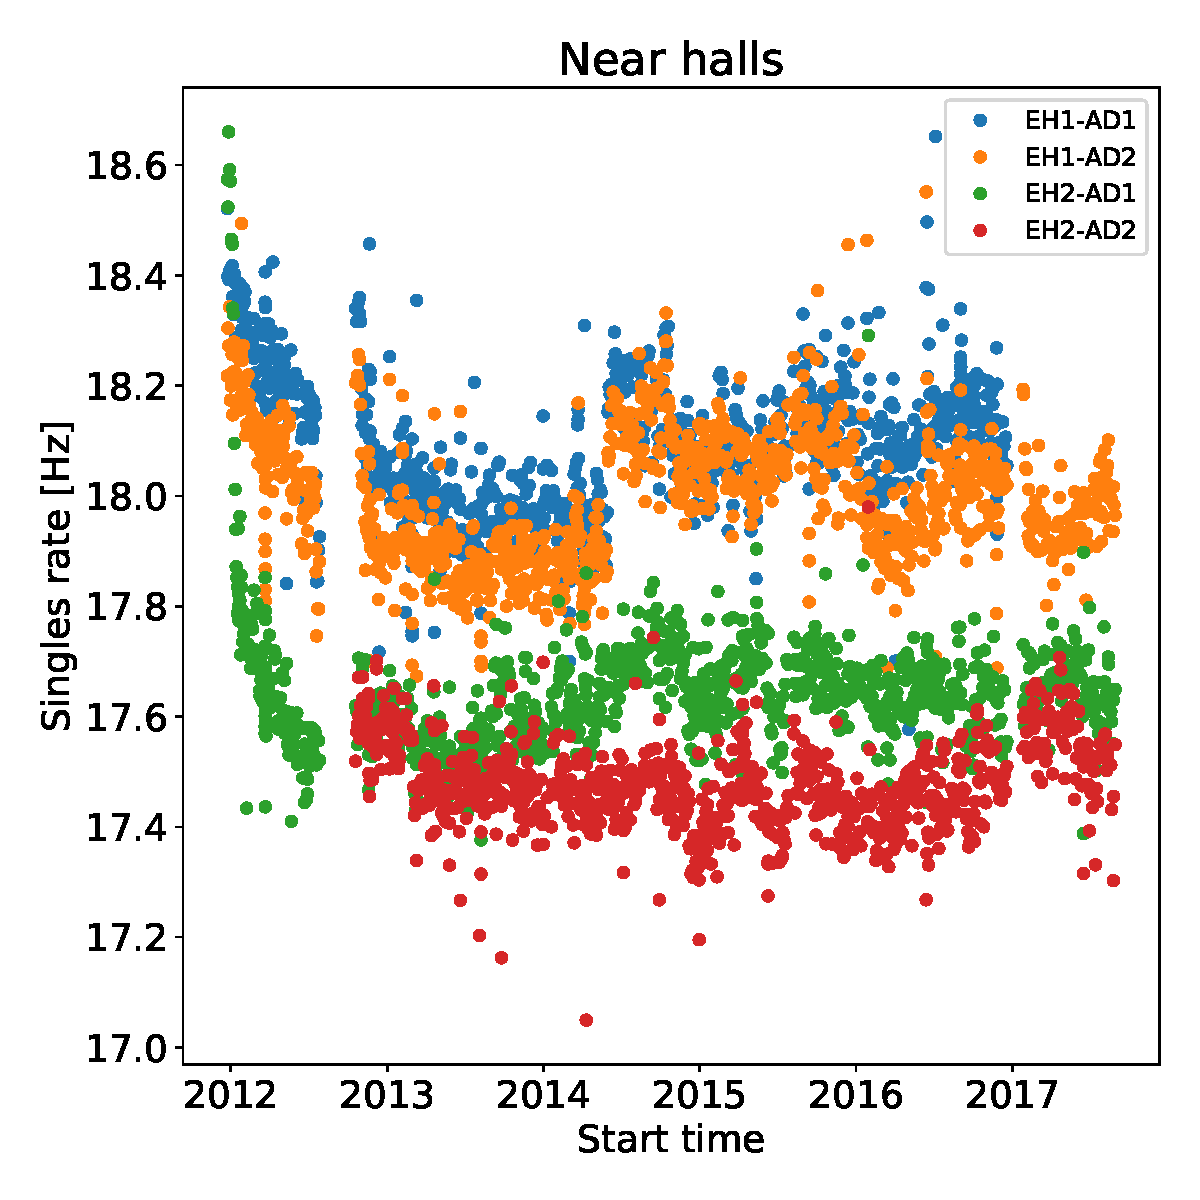
\includegraphics[width=0.48\textwidth]{plot_diagnostics/singles_near_bydate}
    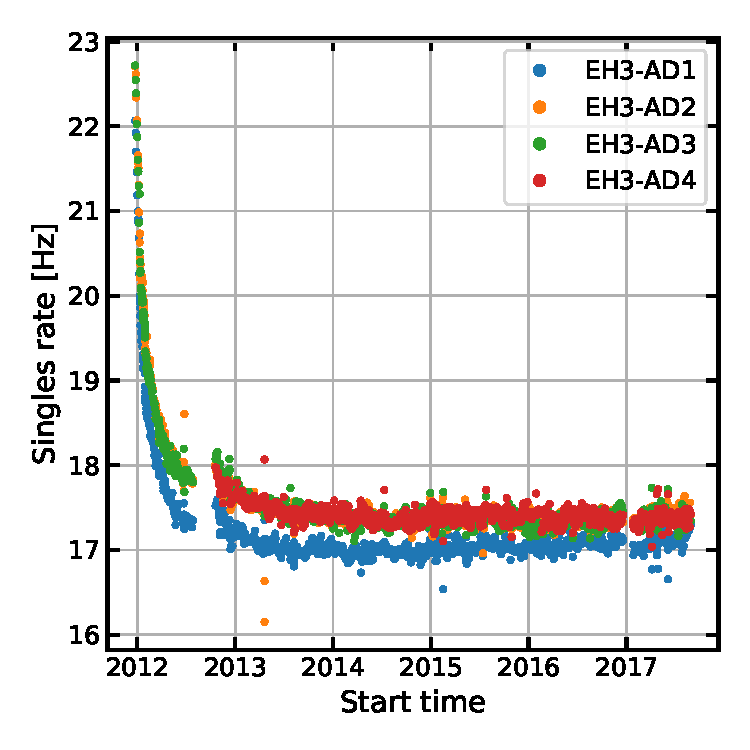
\includegraphics[width=0.48\textwidth]{plot_diagnostics/singles_far_bydate}
    \caption[Singles rate over time]{
        Singles rate $R_s$ over time for
        the near halls (top) and far hall (bottom).
        Each data point represents one data run.
    }
    \label{fig:singles}
\end{figure}

The uncorrelated event rate $R_s$ for the near and far halls is shown in
\cref{fig:singles}.
$R_s$ was higher when the experiment began because
the dark rate of the PMTs had not yet stabilized
and long-lived
radioactive contaminants had not yet decayed away.
In particular, the far-hall ADs EH3-AD1, EH3-AD2, and EH3-AD3
were filled shortly before physics data taking began,
while the near-hall ADs EH1-AD1, EH1-AD2, and EH2-AD1
were filled and then studied for a few months
as part of detector commissioning, during which time
most of the radiocontaminants decayed.

\subsection{Accidental coincidence rate}
\label{subsec:2fold}

Once $R_s$ was obtained, $R_{\text{\fold{2}}}$ was computed for each run
as the rate of accidental coincidences of two uncorrelated events within \tc{},
with energies between \SIlist{1.5;12}{\MeV}, and with no DT restriction.
The value of $R_\text{\fold{2}}$ is given by
\begin{equation}
    \label{eq:racc}
        R_{\text{\fold{2}}} = R_s\tc R_{\text{\fold{1}}},
\end{equation}
as derived in \cref{ap:singlesformula}.
The rate $R_{\text{\fold{2}}}$ obtained from this formula
could not simply be subtracted from the measured \fold{2} rate
to obtain $R_{\text{IBD}}$,
since this rate was computed without accounting
for the delayed energy cut or the DT cut.

\subsection{Synthetic accidentals}
\label{subsec:synthetic}

Characterization of the delayed energy and DT properties
of the accidental background
was performed in a data-driven manner using
a synthetic sample of accidental events.
The synthetic coincidences were constructed out of a sample of isolated single events,
similar to the sample used in the computation of $R_\text{\fold{2}}$.
However, a stricter isolation cut was used for this part of the study
to increase the purity of the sample.
This was acceptable because the energy and position characteristics of uncorrelated events
by definition did not change based on the presence or absence
of surrounding events.
Only \fold{1} events which had no preceding events within \SI{1.5}{\ms}
were accepted into this sample
to ensure isolation before and after each candidate event.
The spectrum of these (now truly) single events is shown in \cref{fig:singlespectra},
obtained by summing the individual spectra from each data run for each AD.

\adgrid[0.22\textheight]{
    Spectra of isolated single events in each AD
    used to construct the synthetic accidentals samples.
    This sample included all events passing the following cuts: muon veto,
    flasher, prompt energy, and the time isolation cut of \SI{\pm1.5}{\ms}.
}{fig:singlespectra}{ch_background/singles}{
    Single events spectrum
}

A synthetic accidentals sample was created for each run
by pairing up the isolated events.
In particular, each event was assigned an index in time order,
from $0$ to $N_{\text{isolated}}$.
Then each event $i$ from the first half of the run was paired with
the corresponding event from the second half, $i + N_{\text{isolated}}2$.
The large time separation between the two events
ensured that they were truly uncorrelated.
The synthetic coincidence distance was taken to be the actual distance
between the reconstructed positions of the two events.
The synthetic coincidence time was drawn at random
from the coincidence time distribution
expected from true accidental coincidences.

\subsection{Contamination of IBD sample}
\label{subsec:acc_count}

The total accidentals efficiency $\varepsilon_\text{total,\,acc}$
was defined as the fraction of accidental \fold{2} coincidences
that passed the full IBD selection including energy cuts and DT cuts,
estimated from the synthetic accidentals sample as
\begin{equation}\label{eq:eps_total_acc}
    \varepsilon_{\text{total,\,acc}} =
    \frac{N_\text{acc}'[E_p \wedge E_d \wedge \text{DT}]}{N_\text{acc}'[E_p]},
\end{equation}
where $N_\text{acc}'[\cdot]$ refers to the number of events
in the synthetic accidentals sample satisfying certain selection criteria.
The total expected number of accidental coincidence events
that passed the full IBD selection was then computed
separately for each run, and the counts for all the runs for each AD were combined:
\begin{align}\label{eq:nacc}
    \begin{split}
        N_{\text{acc},r} &= R_{\text{\fold{2}},r}
            \times T_{\text{DAQ},r}\times \varepsilon_{\mu,r}
            \times \varepsilon_{\text{total,\,acc},r}\\
        N_\text{acc} &= \sum_r N_{\text{acc},r}
    \end{split}
\end{align}
where $r$ indexes over all runs for a given AD
and $\varepsilon_\mu$ is defined in \cref{eq:muon_eff}.
Note that the multiplicity veto efficiency $\varepsilon_m$,
which must be explicitly included in all other rate-to-counts conversions,
is implicitly present in the computation of $R_\text{\fold{2}}$.
After all, any accidental coincidences which were multiplicity-vetoed
by another uncorrelated event were actually \fold{3} accidental coincidences,
and thus were already excluded from $R_\text{\fold{2}}$.

\subsection{Accidentals rate uncertainty}
\label{subsec:acc_err}

The uncertainty assigned to the accidentals contamination $N_\text{acc}$
was dominated by the statistical uncertainty in the subtraction procedure.
A thorough characterization of the systematic uncertainty
was also undertaken.

\subsubsection{Statistical uncertainty}

The uncertainty of $N_{\text{acc}}$ due to the finite statistics
of the synthetic accidentals sample
and in counting $N_{\text{\fold{1}}}$ (to extract $R_s$)
was computed for each run based on \cref{eq:nacc}
and the standard propagation of errors,
and the results from each run were combined in quadrature.
The \fold{2} coincidence rate, $R_\text{\fold{2}}$,
was derived from a counting measurement of $N_\text{\fold{1}}$,
whose relative uncertainty was
\begin{equation}\label{eq:sigma_1fold}
    \frac{\sigma_\text{\fold{1}}}{N_\text{\fold{1}}} =
    \frac{1}{\sqrt{N_\text{\fold{1}}}}.
\end{equation}
Note that the relative uncertainty on the rate
$R_\text{\fold{1}} = N_\text{\fold{1}}/(T_\text{DAQ}\varepsilon_\mu)$ was identical.
The uncertainty on $R_s$ was computed numerically
based on \cref{eq:rsingles} to be
\begin{equation}\label{eq:sigma_rs}
    \sigma_s \approx 1.1\times\sigma_\text{\fold{1}}.
\end{equation}
To obtain the uncertainty on $R_\text{\fold{2}}$ based on \cref{eq:racc},
the uncertainties on $R_\text{\fold{1}}$ and $R_s$ were combined linearly
since the two values were highly correlated; thus
\begin{equation}\label{eq:sigma_2fold}
    \frac{\sigma_\text{\fold{2}}}{R_\text{\fold{2}}} \approx
    \frac{2.1}{\sqrt{N_\text{\fold{1}}}}.
\end{equation}
Finally, the uncertainty on the efficiency $\varepsilon_\text{total,\,acc}$
was computed using the binomial distribution to be
\begin{equation}\label{eq:sigma_eps_acc}
    \sigma_{\varepsilon_\text{total,\,acc}} =
    \sqrt{
        \frac{
            \varepsilon_\text{total,\,acc} (1 - \varepsilon_\text{total,\,acc})
        }{N_\text{acc}'}
    }.
\end{equation}
Thus the total uncertainty on the number of accidental events
for a given run based on \cref{eq:nacc} was
\begin{equation}\label{eq:sigma_acc}
    \frac{\sigma_\text{acc}^2}{N_\text{acc}^2} \approx
    \frac{2.1^2}{N_\text{\fold{1}}}
    + \frac{1-\varepsilon_\text{total,\,acc}}{
        \varepsilon_\text{total,\,acc} N_\text{acc}'
    }.
\end{equation}
For a typical 24-hour run at any of the ADs,
the overall statistical uncertainty was approximately \SI{3}{\percent}.
These statistics were uncorrelated between runs,
so the total relative uncertainty was suppressed
when the runs were combined according to \cref{eq:nacc},
and are listed in \cref{tab:summary_event_selection}
with values of \SI{\sim0.08}{\percent} for each AD.

\subsubsection{Systematic uncertainty}

Studies were performed to constrain the possible deviation
of the true accidentals rate
from the rate extracted using the above procedure.
Such an error would affect the IBD rates at the near and far ADs in different proportions,
leading to a bias in \thetaot{}.
In fact, using the accidental and IBD event counts in \cref{tab:summary_event_selection},
it can be shown that a bias of $b\si{\percent}$ in $N_{\text{acc}}$
would yield a bias in $N_{\text{IBD}}$ of $-1b\si{\percent}$ at the far site
but only $-0.13b\si{\percent}$ at the near sites.
For example, in EH3-AD1 there were \num{162005} IBD candidates,
of which \num{79658} were expected to be accidental coincidences,
leaving \num{82347} correlated events.
If the accidentals prediction were \SI{1}{\percent} higher (\num{80455}),
the new extracted number of correlated events would be \num{81550},
which is \SI{-0.97}{\percent} of the nominal value.
A similar computation for EH1-AD1 results in a change of only \SI{-0.13}{\percent}.

The accuracy of the method used to compute $R_{s}$,
the primary input to $R_{\text{\fold{2}}}$,
was examined using the Reconstructed-Data File Simulation described in \cref{sec:toymc}.
The results of the simulation study verified that
the above method extracts $R_s$ with high accuracy, at worst biased by \SI{0.02}{\percent}.
In particular, the treatment of the small correlated event rate as negligible
is validated as an appropriate approximation.

The implicit assumption of a constant $R_s$ within a given run was also tested.
The validity of this assumption was enhanced by the near-linearity of
the dependence of $R_{\text{\fold{2}}}$ on $R_s$;
if the relation were purely linear,
then the average of $R_s$ within a run could be used to exactly compute
the average $R_{\text{\fold{2}}}$ since averaging is a linear transformation.
Hourly singles rates were computed, and deviations of up to \SI{4}{\percent}
were found within runs.
For a typical value of $R_s$ of \SI{18}{\Hz},
and the worst-case scenario of half the run at a \SI{4}{\percent} excess
and half the run at a \SI{4}{\percent} deficit,
the impact on $R_{\text{\fold{2}}}$ would be \SI{\sim0.04}{\percent}.

The method of generating a synthetic accidentals sample
by pairing up isolated single events was examined using actual data.
The specific pairing algorithm, which pairs events from the first half of a run
with events from the second half of a run,
could create a synthetic sample not representative of the true accidental background
if the properties of uncorrelated events changed significantly during a run.
An alternate pairing algorithm was designed to pair isolated events
chosen at random (without replacement) from the set of singles from a given run.
Values of $\varepsilon_{\text{DT,\,acc}}$ (defined in \cref{subsec:delayed}) were extracted from each pairing algorithm.
The average deviation between the two algorithms' values was within \SI{0.15}{\percent};
however, this was partially attributed to the finite statistics
of the synthetic accidentals sample
and so was not necessarily indicative of a major source of systematic uncertainty.

A final study was performed to test the full procedure
for extracting the accidental background contamination.
Rather than predicting the number of accidental coincidences
contaminating the IBD sample,
the procedure was adapted to predict the number of accidental coincidences
which failed the DT cut.
This sample was cleanly isolated from IBDs and correlated backgrounds
by selecting double coincidence events with $\text{DT} > \SI{3000}{\mm}$,
and with prompt and delayed energy between \SIlist{1.5;12}{\MeV}.
The same selection cuts were applied to the synthetic accidental sample,
replacing $\varepsilon_\text{total,\,acc}$ with $\varepsilon_\text{DT,\,acc}$
to account for the weaker constraint on the delayed energy.
The results for the synthetic sample were input into \cref{eq:nacc} to obtain
the predicted number of accidentals with $\text{DT} > \SI{3000}{\mm}$.
In all ADs, the number of such events
agreed with the observed number of events
to within \SI{0.04}{\percent};
\cref{tab:acc_validation} lists the observed and predicted values
for each AD.
\Cref{fig:DT_sub} shows the DT parameter distributions in EH3-AD4
for the data sample, the synthetic accidentals sample,
and the difference between them
showing the close agreement for DT values above a few meters.
This agreement tightly constrained possible systematic biases
in the computation of the accidental background.
The only assumption underlying this constraint on the systematic uncertainty
was that the synthetic accidentals sample
predicted the true accidentals' DT distribution as well at $\text{DT} < \SI{800}{\mm}$
as it did over the broad range $\SI{3000}{\mm} < \text{DT} < \SI{10000}{\mm}$.

\begin{table}[ht]
    \centering
    \caption[Validation of accidentals rate]{
        Comparison between actual and predicted
        accidental coincidences whose DT parameters
        fall between \SIlist{3;10}{\m}.
        The tilde ($\tilde{N}$) indicates that these are not counts of IBD candidates.
        See the text for a detailed description.
    }
    \label{tab:acc_validation}
    \begin{tabular}[t]{
        l
        S[
            table-number-alignment = center,
            table-figures-decimal = 0,
            table-figures-integer = 8
        ]
        S[
            table-number-alignment = center,
            table-figures-decimal = 0,
            table-figures-integer = 8
        ]
        S[
            table-number-alignment = center,
            table-figures-decimal = 0,
            table-figures-integer = 5,
            table-sign-mantissa = true,
        ]
        S[
            table-number-alignment = center,
            table-figures-decimal = 3,
            table-figures-integer = 1,
            table-sign-mantissa = true,
        ]
    }
        \toprule
        & {$\tilde{N}_\text{obs}$}
        & {$\tilde{N}_\text{acc}'$}
        & {$\tilde{N}_\text{acc}' - \tilde{N}_\text{obs}$}
        & {$\frac{\tilde{N}_\text{acc}' - \tilde{N}_\text{obs}}{\tilde{N}_\text{obs}}$}
        [\%]\\
        \midrule
        EH1-AD1 & 30992521 & 30999739 & 7218 & 0.023 \\
        EH1-AD2 & 34532571 & 34533421 & 850 & 0.003 \\
        EH2-AD1 & 36780355 & 36775698 & -4656 & -0.013 \\
        EH2-AD2 & 32326145 & 32313935 & -12209 & -0.038 \\
        EH3-AD1 & 47984334 & 47982715 & -1618 & -0.003 \\
        EH3-AD2 & 50072382 & 50069291 & -3090 & -0.006 \\
        EH3-AD3 & 50089966 & 50086848 & -3117 & -0.006 \\
        EH3-AD4 & 43983829 & 43966224 & -17604 & -0.040 \\
        \bottomrule
    \end{tabular}
\end{table}

\begin{figure}
    \centering
    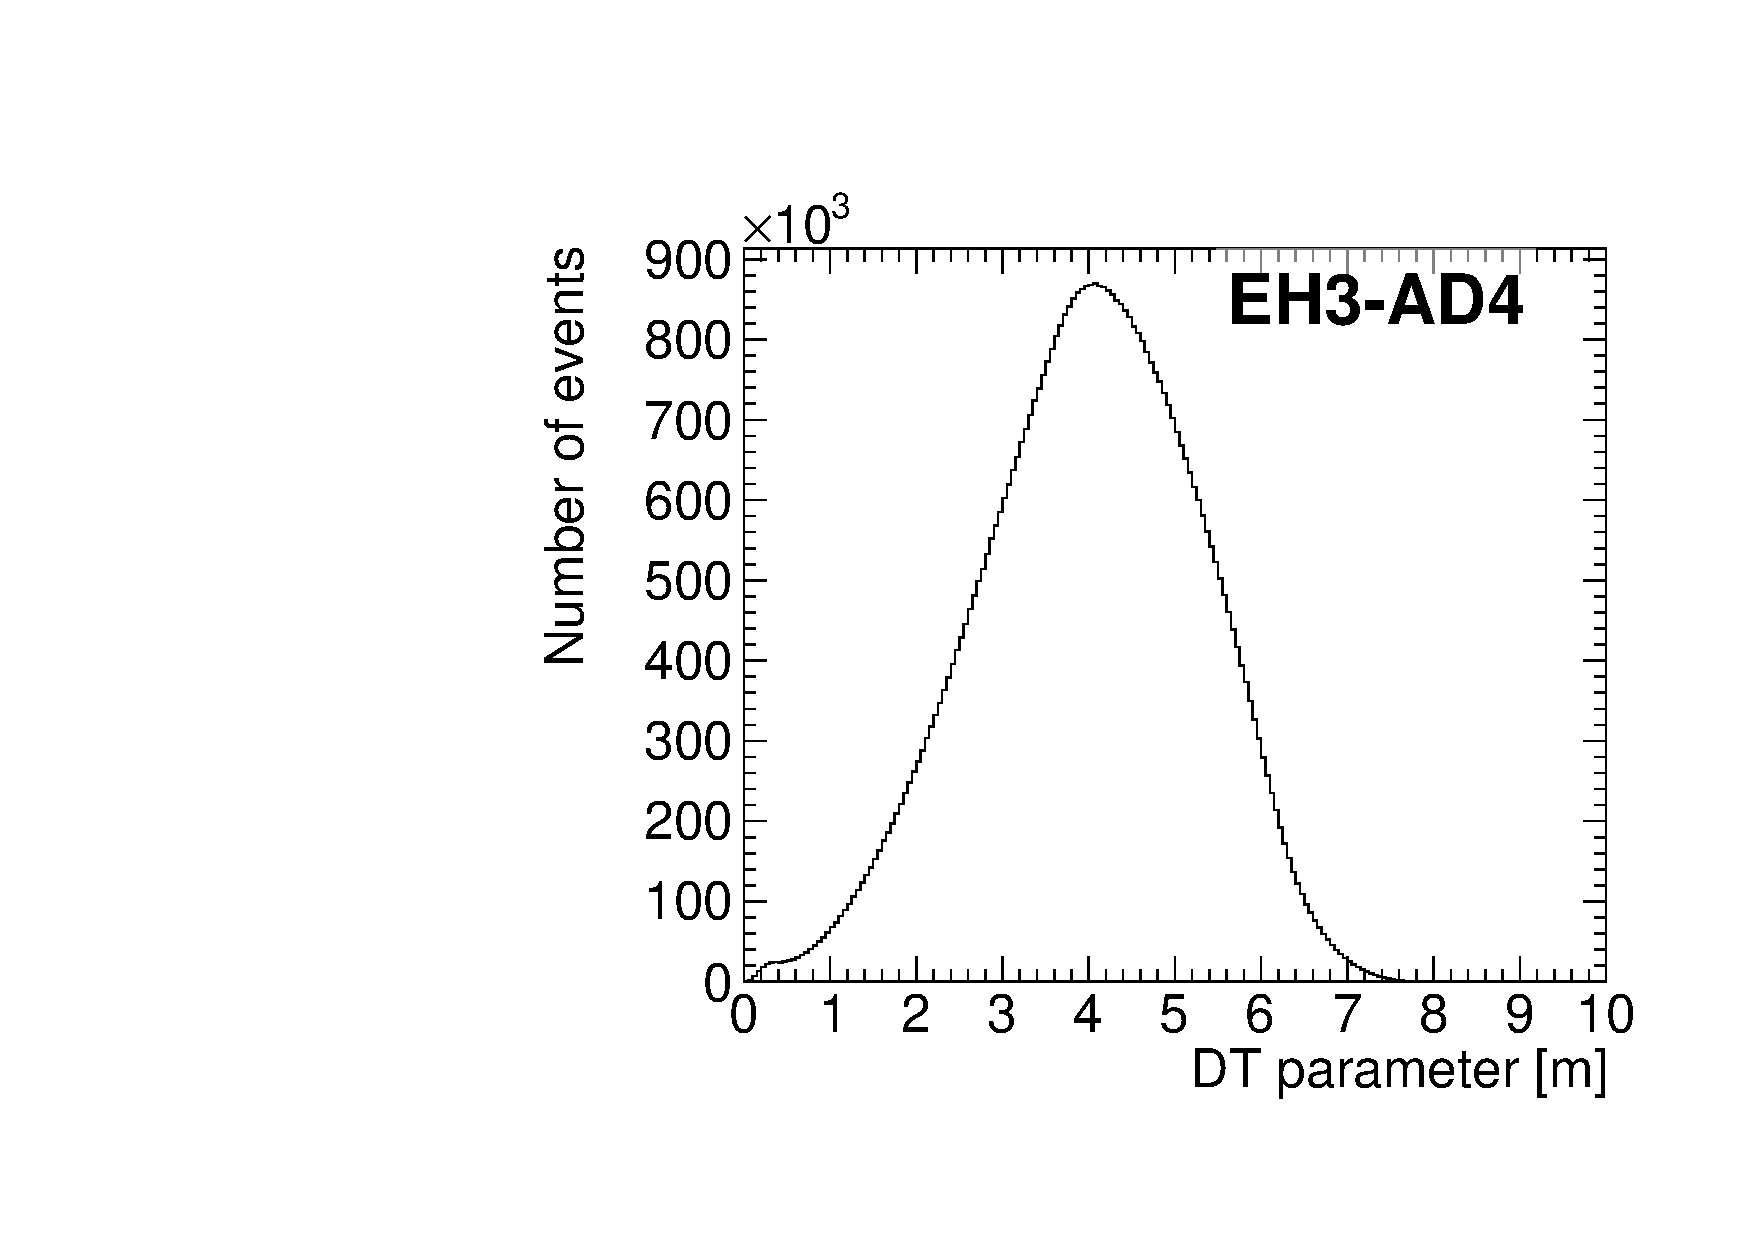
\includegraphics[width=0.49\textwidth]{ch_event_selection/DT_data_EH3_AD4}
    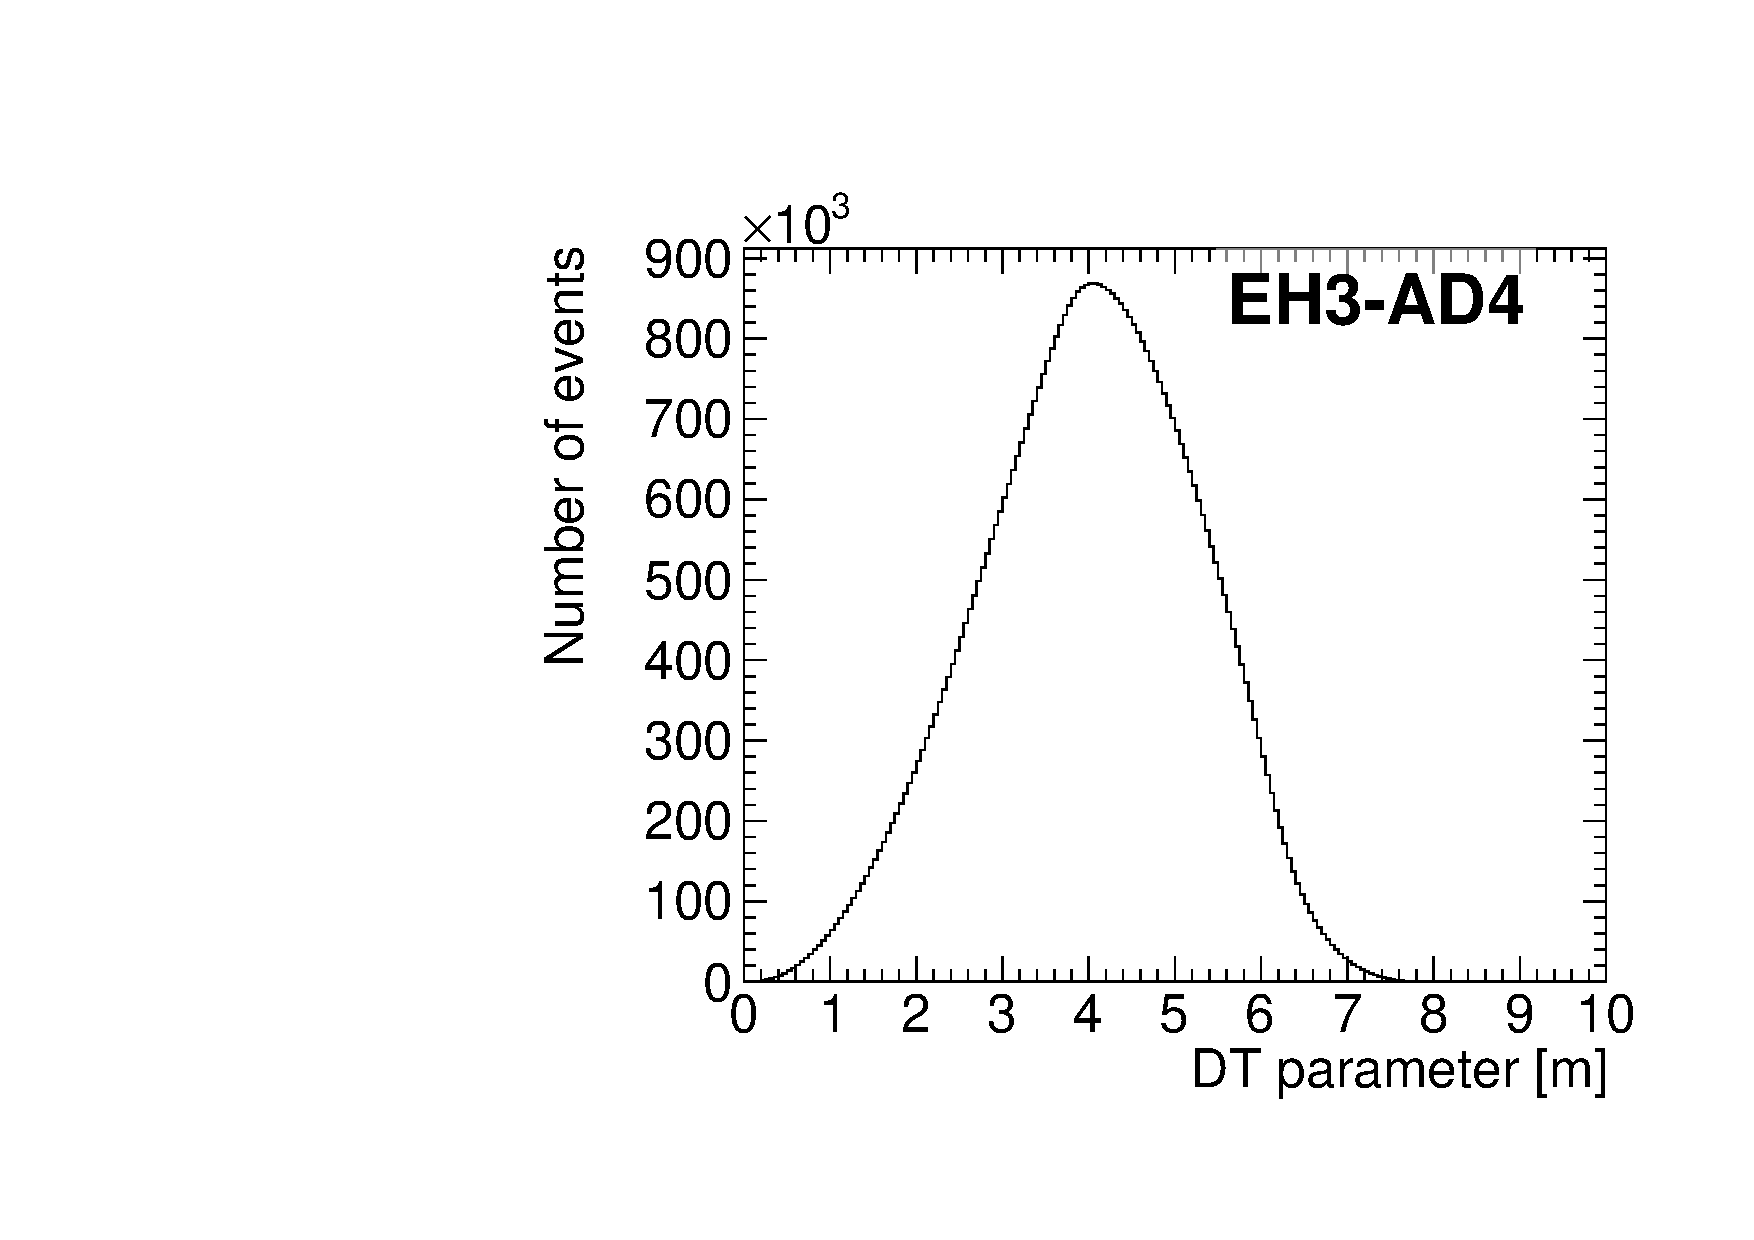
\includegraphics[width=0.49\textwidth]{ch_event_selection/DT_bg_EH3_AD4} \\
    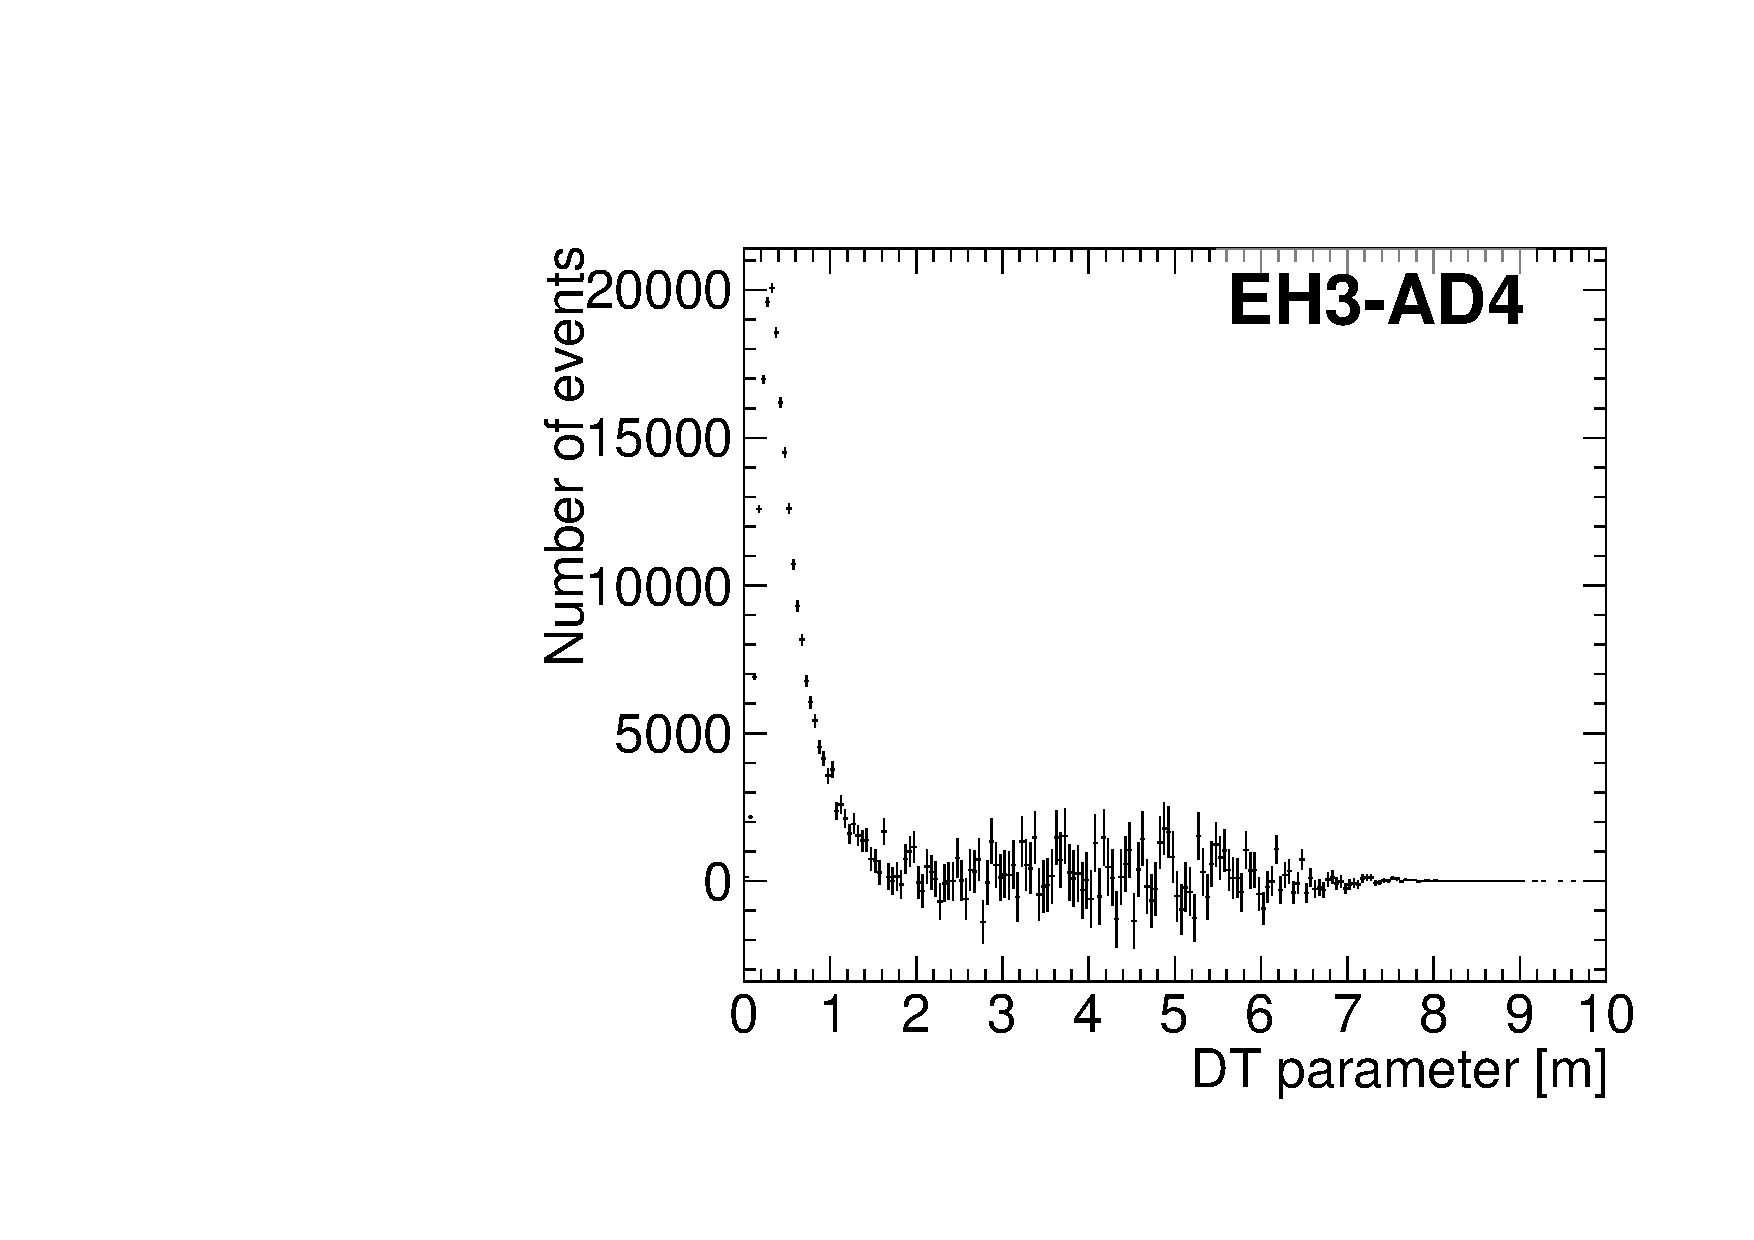
\includegraphics[width=0.49\textwidth]{ch_event_selection/DT_sub_EH3_AD4}
    \caption[Validation of accidentals rate]{
        Distribution of the DT parameter used to constrain
        the systematic uncertainty in the accidental background rate in EH3-AD4
        (similar in all ADs).
        Top left: double coincidences (data), identical to \cref{fig:DT_data}.
        Top right: synthetic accidentals (prediction).
        Bottom: difference between the double coincidences and synthetic accidentals.
        The data and prediction differ by only \SI{0.04}{\percent}
        between \SIlist{3;10}{\m}.
    }
    \label{fig:DT_sub}
\end{figure}

Based on these studies, the systematic uncertainty
due to the procedure for determining the number of accidental events $N_{\text{acc}}$
was taken to be \SI{0.04}{\percent},
which was sub-dominant compared to the statistical uncertainty of \SI{0.08}{\percent},
and negligible when considered along with
the uncertainties on the other irreducible backgrounds
as described in \cref{sec:correlated_bg}.

\section{Delayed energy}
\label{subsec:delayed}

Neutron capture on hydrogen (nH) released a single
\SI{2.22}{\mev} $\gamma$-ray,
which allowed the delayed-energy cut bounds to be tuned to a narrow energy region
around that value.
However, emitted $\gamma$-rays occasionally
deposited less than their full energy in the liquid scintillator,
as shown in \cref{fig:prompt_eff_mc} by the extended low-energy tail
below \SI{2.22}{\MeV} and by the peak at 0 energy,
representing events where the $\gamma$-ray escaped entirely.
Both the tuning of the energy cut
and the fraction of escaping $\gamma$-rays were sensitive to
small variations in the geometry of the AD, energy reconstruction,
and scattering properties of $\gamma$-rays in
both liquid scintillator and in acrylic.

The delayed-energy cut bounds were identified based on
functions fitted to each AD's delayed energy spectrum.
The measured delayed energy spectrum was obtained by first applying
the prompt energy cut and DT cut,
then statistically subtracting the accidental background
using the same synthetic accidental coincidence sample
discussed in \cref{sec:acc}.
From this synthetic accidental coincidence sample, $\varepsilon_{\text{DT,\,acc}}$,
the fraction of accidental \fold{2} coincidences which passed the distance-time (DT) cut
and prompt energy cut, was computed:
\begin{equation}\label{eq:eps_DT_acc}
    \varepsilon_{\text{DT,\,acc}} =
    \frac{N_\text{acc}'[E_p \wedge \text{DT}]}{N_\text{acc}'[E_p]}.
\end{equation}
A prompt-delayed energy spectrum was generated that only included
synthetic accidental events which passed the DT cut,
as shown in \cref{fig:acc_sample}.
Each event in the synthetic sample generated two entries to this histogram:
one with the event from the first half of the run as the prompt event,
and one with that event as the delayed event,
to increase the statistical precision of the spectrum.
\adgrid[0.22\textheight]{
    Prompt-delayed spectra of the synthetic accidentals sample
    after applying the DT cut.
    Each 2D plot is symmetrical under interchange of prompt and delayed energy
    by construction, since each synthetic pair is added to the histogram twice.
    The plots may not appear to be perfectly symmetrical
    due to artifacts of the plotting software.
}{fig:acc_sample}{ch_background/acc}{
    Prompt-delayed spectrum: synthetic accidentals
}

The resulting prompt-delayed energy spectrum of synthetic accidental events
for each run was then subtracted
from the prompt-delayed spectrum measured from real data
after also applying the DT cut, as shown in \cref{fig:after_DT_cut}.
For each run, the expected number of accidental coincidences
with prompt and delayed energies between \SIlist{1.5;12}{\MeV}
that passed the DT cut was
\begin{equation}
    N_{\text{acc,\,loose}} = R_{\text{\fold{2}}}
        \times T_\text{DAQ}\times \varepsilon_\mu
        \times \varepsilon_{\text{DT,\,acc}}
    \label{eq:nacc_loose}
\end{equation}
The synthetic accidentals prompt-delayed spectrum, represented as a histogram,
was normalized so that the integral was $N_{\text{acc,\,loose}}$.
Then the histogram was subtracted bin-by-bin from the corresponding histogram
representing the actual double coincidence data sample.
The subtracted histograms are shown in \cref{fig:acc_sub_spectra}.

\adgrid[0.22\textheight]{
    Prompt-delayed spectra after subtracting the accidental background.
    The projections of these plots onto the delayed energy axis
    were used to determine the delayed energy cut bounds
    and are shown in \cref{fig:delayed_fits}.
}{fig:acc_sub_spectra}{ch_background/sub_energy}{
    Prompt-delayed spectrum: after subtracting accidentals
}

Although the accidentals-subtracted spectrum was still not pure IBDs,
the only remaining backgrounds were due to correlated processes
where the delayed event is still
neutron capture on hydrogen, and thus
the delayed energy spectrum at this point
consisted solely of nH captures.

The projections of these 2D spectra onto the delayed energy axis
were fit with the calorimeter function, which models
a calorimetric response to a monoenergetic process with ``true''
energy $\mu$ \cite{calorimeter2016}.
The modeled detector had an intrinsic energy resolution $\sigma$
which applied a Gaussian smearing to the deposited energy.
($\sigma$ itself is independent of energy in this model.)
The model accounted for some fraction $\alpha$ (the peak fraction)
of events being fully contained,
with the remainder of the events partially or fully escaping from the detector.
The energy leakage was modeled as an exponential distribution
with characteristic energy scale (or ``tail slope'') $\lambda$.
The fitting function itself was derived starting with
the unsmeared model:
\begin{equation}
    f_{unsmeared}(E;\mu,\lambda,\alpha) =
    \begin{cases}
        \alpha\delta(E-\mu) + (1-\alpha)\lambda e^{\lambda E}
        & 0 < E \leq \mu \\
        0 & E > \mu
    \end{cases}
\end{equation}
This function was then convolved with a Gaussian
of width $\sigma$:
\begin{align}
    \begin{split}
    f_{cal}    &= f_{unsmeared} \otimes \text{Gaussian} \\
    f_{cal}(E;\mu,\sigma,\lambda,\alpha) &= \int_0^\mu dE'
    f_{unsmeared}(E';\mu,\lambda,\alpha) \cdot \text{Gaussian}(E'-E; \sigma) \\
               &= \frac{1}{\sigma\sqrt{2\pi}}
               \left[
                   \alpha\int_0^\mu dE' e^{-\frac{(E'-E)^2}{2\sigma^2}} \delta(E'-\mu)
                   + (1-\alpha)\int_0^\mu dE' e^{-\frac{(E'-E)^2}{2\sigma^2}}
                   \lambda e^{\lambda E'}
               \right] \\
               &= \alpha\frac{1}{\sigma\sqrt{2\pi}}e^{-\frac{(E-\mu)^2}{2\sigma^2}}
               + (1-\alpha)
               \frac{\lambda e^{\sigma^2\lambda^2+2\lambda E}}{e^{\lambda\mu}-1}
               \left[
                   \text{erf}
                   \left(
                       \frac{\mu-E-\sigma^2\lambda}{\sigma\sqrt{2}}
                   \right)
                   \right. \\
               &\ \ \left.
                   + \text{erf}
                   \left(
                       \frac{E + \sigma^2\lambda}{\sigma\sqrt{2}}
                   \right)
               \right].
    \end{split}
\end{align}
The entire result could then be scaled
by an additional normalization parameter $N$
to match the normalization of the data being fitted.

\adgrid{
    Delayed energy spectrum (data points)
    with the best fit calorimeter function (red curve)
    superimposed, for each AD.
}{fig:delayed_fits}{ch_event_selection/delayed_fit}{
    nH capture delayed energy spectrum
}

\begin{figure}
    \centering
    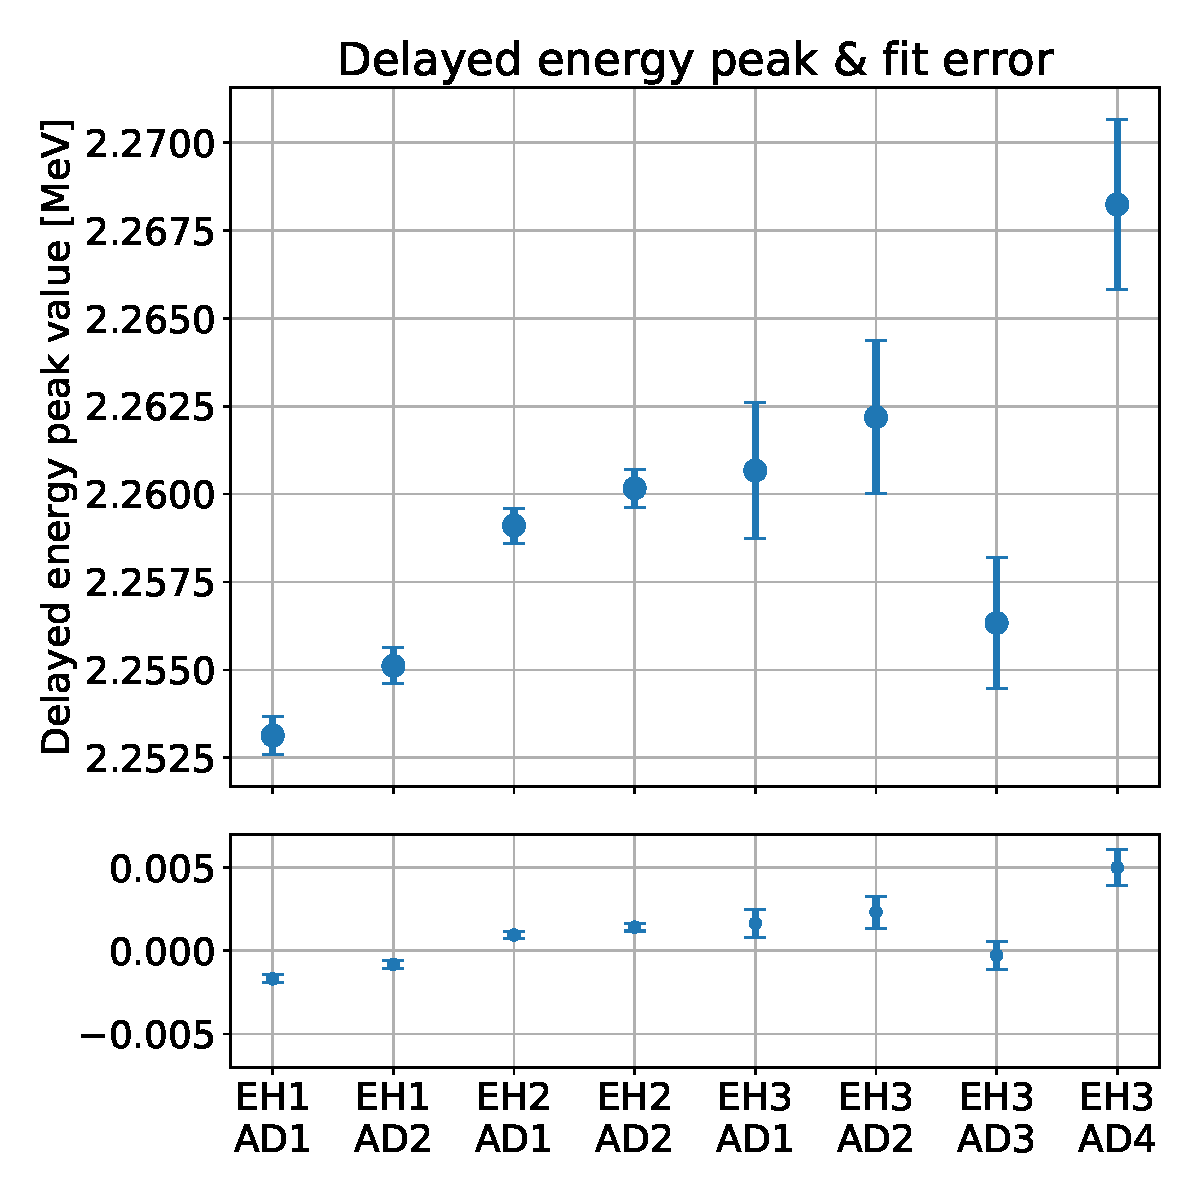
\includegraphics[height=0.33\textheight]{plot_diagnostics/delayed_energy_peak.pdf}
    \vspace{0.5cm}\hspace{0.5cm}
    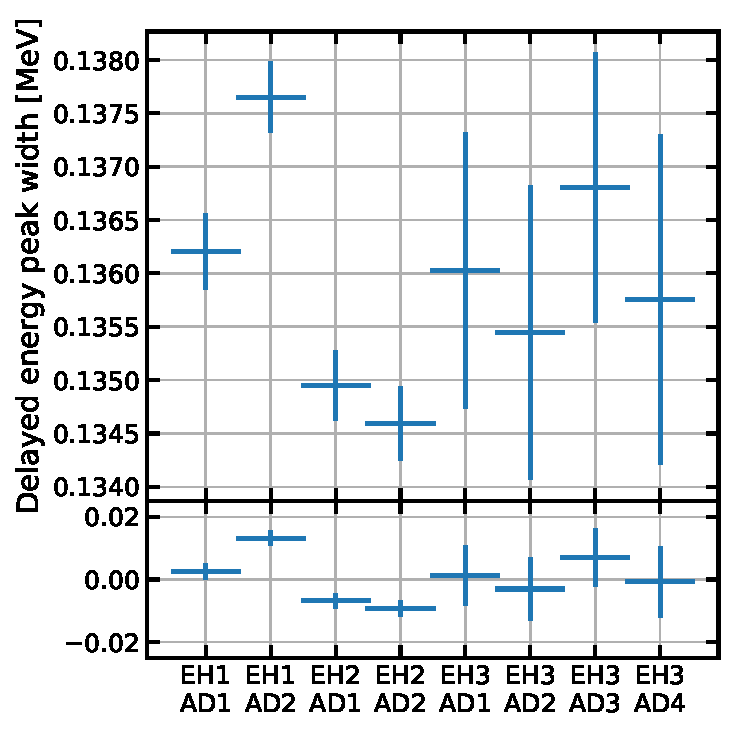
\includegraphics[height=0.33\textheight]{plot_diagnostics/delayed_energy_width.pdf}\\
    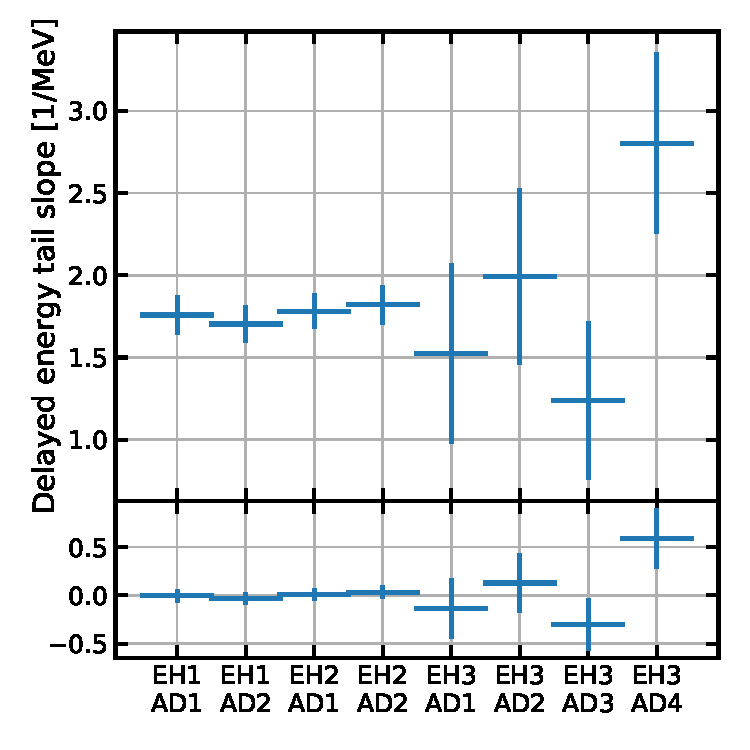
\includegraphics[height=0.33\textheight]{plot_diagnostics/delayed_energy_expo_scale.pdf}
    \hspace{0.5cm}
    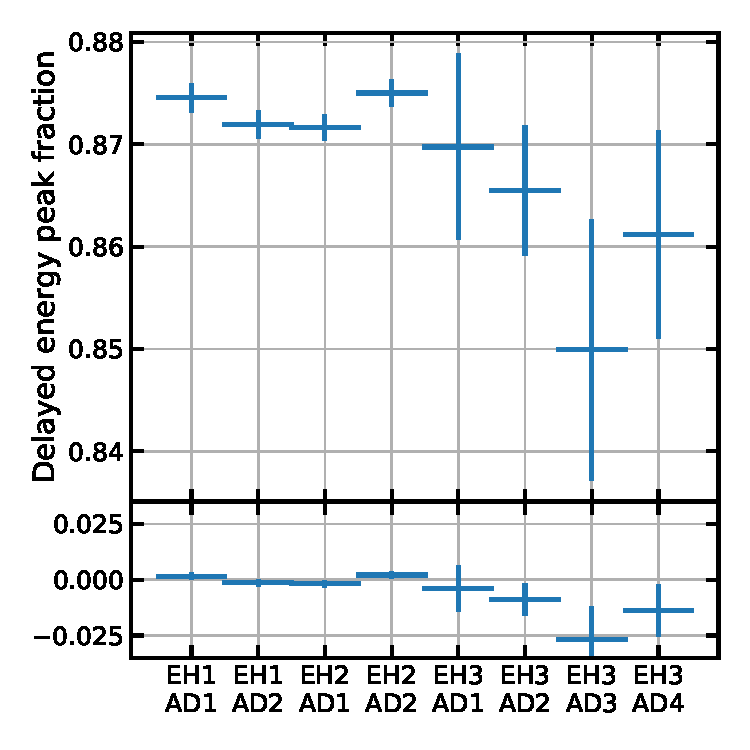
\includegraphics[height=0.33\textheight]{plot_diagnostics/delayed_energy_peak_frac.pdf}\\
    \caption[Delayed energy fit parameters]{
        Fit parameters for each AD.
        Error bars represent fit errors.
        The lower panel of each plot shows the relative deviation of each AD's value
        from the average value of the 4 near-hall ADs.
    }

    \label{fig:delayed_fit_parameters}
\end{figure}

\begin{table}[ht]
    \centering
    \begin{tabular}[t]{lSSSS}
        \toprule
        & {Peak energy [\si{\mev}]}
        & {Width [\si{\mev}]}
        & {Tail slope [\si{\per\mev}]}
        & {Peak fraction} \\
        \midrule
        EH1-AD1 & 2.2531 & 0.1365 & 1.6893 & 0.8683\\
        EH1-AD2 & 2.2551 & 0.1380 & 1.6247 & 0.8666\\
        EH2-AD1 & 2.2591 & 0.1351 & 1.7212 & 0.8663\\
        EH2-AD2 & 2.2602 & 0.1348 & 1.7319 & 0.8902\\
        \addlinespace
        EH3-AD1 & 2.2607 & 0.1360 & 1.5812 & 0.8667\\
        EH3-AD2 & 2.2622 & 0.1349 & 2.1516 & 0.8616\\
        EH3-AD3 & 2.2563 & 0.1366 & 1.3432 & 0.8507\\
        EH3-AD4 & 2.2682 & 0.1362 & 2.5653 & 0.8617\\
        \bottomrule
    \end{tabular}
    \caption[Delayed energy fit parameters]{Delayed energy fit parameters.}
    \label{tab:delayed_fit_params}
\end{table}

\begin{table}[ht]
    \centering
    \begin{tabular}[t]{lSS}
        \toprule
        & {Lower bound [\si{\mev}]}
        & {Upper bound [\si{\mev}]} \\
        \midrule
        EH1-AD1 & 1.8435 & 2.6628\\
        EH1-AD2 & 1.8412 & 2.6690\\
        EH2-AD1 & 1.8537 & 2.6645\\
        EH2-AD2 & 1.8558 & 2.6646\\
        \addlinespace
        EH3-AD1 & 1.8527 & 2.6686\\
        EH3-AD2 & 1.8575 & 2.6669\\
        EH3-AD3 & 1.8467 & 2.6660\\
        EH3-AD4 & 1.8597 & 2.6768\\
        \bottomrule
    \end{tabular}
    \caption[Delayed-energy cut bounds]{
        Delayed-energy cut bounds derived as $\mu \pm 3\sigma$.
    }
    \label{tab:delayed_bounds}
\end{table}

\begin{figure}
    \centering
    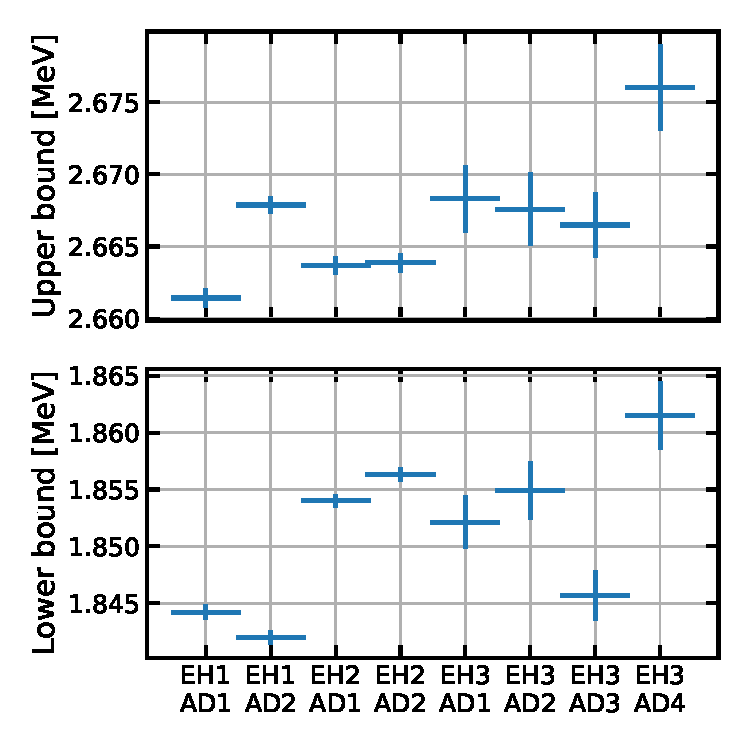
\includegraphics[height=0.40\textheight]{plot_diagnostics/delayed_energy_bounds.pdf}
    \caption[Delayed energy cut bounds]{
        Delayed energy cut bounds computed as $\mu\pm 3\sigma$
        from the fitted histograms.
    }
    \label{fig:delayed_bounds}
\end{figure}

The eight delayed energy spectra with their fits are shown in \cref{fig:delayed_fits}.
The values and relative differences of the fitted parameters
are plotted in \cref{fig:delayed_fit_parameters},
and the values are listed in \cref{tab:delayed_fit_params}.
In particular, the top-left plot shows the relative difference
in the fitted peak energy $\mu$ across the ADs,
which is a measure of the energy scale variation (\cref{subsec:rel_energyscale}).
The relative variation of \SI{+-0.5}{\percent}
was interpreted as the relative energy scale uncertainty
(discussed in \cref{subsec:rel_energyscale}).

The bounds for the delayed energy cut were computed
based on the fitted peak value and energy resolution
from the calorimter model.
The energy criterion was
\begin{equation}\label{eq:delayed_cut}
    \mu - 3\sigma < E_d < \mu + 3\sigma.
\end{equation}
This form was decided on even though the calorimeter function
is not symmetric, and even though in reality
the detector resolution changed with energy
(and therefore was not precisely modeled in the fit).
The critical property of this selection criterion was
not the degree to which the model matched the physical process,
but rather whether the efficiency of the cut was similar in all ADs,
as discussed in \cref{subsec:eff_delayed}.
The values used for the delayed-energy cut bounds are listed in \cref{tab:delayed_bounds}
and plotted in \cref{fig:delayed_bounds}.

\section{Selection efficiencies}
\label{sec:efficiencies}

To ensure that the comparison of IBD counts across ADs was meaningful,
the observed counts were corrected
for differences in selection efficiency between ADs,
that is, the probability that a true IBD event
passed all selection criteria in one AD
relative to the probability in another AD.
Where the absolute efficiencies were known with enough precision
(for the muon and multiplicity cuts $\varepsilon_\mu$ and $\varepsilon_m$),
they were used to correct the observed counts of IBD candidates.
In the following, these two efficiencies are implicity carried through
with zero uncertainty.
For the remaining sources of detection inefficiency,
only the relative, uncorrelated variation between ADs was characterized,
since any absolute or correlated component to the efficiencies
would cancel when taking the ratio of corrected counts from two ADs.
The precise values for $\varepsilon_\mu$ and $\varepsilon_m$
are listed in \cref{tab:summary_event_selection},
and the AD-uncorrelated uncertainties for the remaining efficiencies
are listed in \cref{tab:efficiency_summary}.

Selection efficiencies were factored into
contributions from each individual selection cut.
The order that the cuts are applied is in principle arbitrary;
this analysis uses an order
motivated by the intuitive sequence of event selection steps:
prompt energy cut $E_p$, delayed energy cut $E_d$, then DT cut:
\begin{align}\label{eq:efficiency_def}
    \begin{split}
        \varepsilon &= \frac{N_\text{IBD}[E_p \wedge E_d \wedge \text{DT}]}{
            N_\text{IBD}
        } \\
                    &= \frac{N_\text{IBD}[E_p]}{N_\text{IBD}} \times
                    \frac{N_\text{IBD}[E_p \wedge E_d]}{
                        N_\text{IBD}[E_p]
                    } \times
                    \frac{N_\text{IBD}[E_p \wedge E_d \wedge \text{DT}]}{
                        N_\text{IBD}[E_p \wedge E_d]
                    } \\
        \varepsilon &= \varepsilon_\text{prompt}\varepsilon_\text{delayed}
        \varepsilon_\text{DT}.
    \end{split}
\end{align}
The notation $N[A \wedge B]$ means
the number of events accepted after applying cuts $A$ and $B$.
The overall denominator $N_\text{IBD}$
represents the total number of true IBD interactions
that occured on a target proton in the AD,
whether or not they were eventually detected,
and whether or not the neutron captured on Gd or H.
Including nGd events ensured that the analysis of relative efficiencies
accounted for variation in the nGd capture fraction across ADs.
The uncertainty in this value was a primary motivation
for pursuing the purely relative analysis in \cref{ch:analysis}.

\subsection{Prompt energy cut efficiency}
\label{subsec:eff_prompt}

The prompt energy cut efficiency was defined
according to \cref{eq:efficiency_def} as
\begin{equation}\label{eq:prompt_eff}
    \varepsilon_\text{prompt} = \frac{N_\text{IBD}[E_p]}{N_\text{IBD}}.
\end{equation}
The absolute efficiency was estimated using the Individual Event Simulation,
as described in \cref{sec:thu_toymc}, to be \SI{\sim88}{\percent}.
Since the absolute efficiency was not used in the \thetaot{} analysis,
a more precise value was not studied for this thesis.

Because the true \nuebar{} spectrum was different at each AD
due to oscillation effects,
the efficiency of the \SI{1.5}{\MeV} prompt energy cut
was higher at the near ADs than the far ADs
simply due to slightly different spectral shapes \cite{nh2016}.
For example, at shorter baselines, low-energy \nuebar{}'s
were more likely to oscillate to other flavors. At the near halls, then,
there were fewer true IBD events which were rejected by the prompt energy cut
(compared to the no-oscillation assumption),
thus raising the efficiency of the cut.
At the oscillation maximum, though, medium-energy \nuebar{}'s,
around \SIrange{2}{3}{\mev}, were most likely to oscillate (i.e.\ disappear).
Thus the fraction of IBD events with prompt energy above \SI{1.5}{\MeV}
was lower than the no-oscillation prediction.
This relative difference in efficiency between ADs
impacted the extracted value of \thetaot{} by \SI{\sim5}{\percent}.

Corrections for each AD--reactor pair were computed
using the Individual Event Simulation (\cref{sec:thu_toymc})
and weighted to arrive at each AD's final relative prompt-energy efficiency.
Since the corrections to the efficiency depended on
the amplitude of \nuebar{} oscillations, they relied on knowledge of \thetaot.
(For example, there would be no correction at all if \thetaot{} were $0$.)
The correction was defined using the simulated data sample as
\begin{equation}\label{eq:prompt_osc_correction}
    \delta_{p,ik}(\thetaot, \Delta m^2_{32}) =
    \frac{\varepsilon_{\text{prompt},ik}(\thetaot, \Delta m^2_{32})}{
        \varepsilon_{\text{prompt,\,no osc}}
    } - 1,
\end{equation}
where each simulated event in the sample determining the numerator
was weighted by the survival probability
using the baseline between AD $i$ and reactor core $k$.
The no-oscillation efficiency $\varepsilon_{\text{prompt,\,no osc}}$
was common to all AD--reactor pairs.
A grid of correction values in (\thetaot{}, $\Delta m^2_{32}$) parameter space
was pre-computed for use during the fitting process
in \cref{eq:num_ibds_from_core_ij}.
The fitter used linear interpolation to estimate the correction for
a given minimizer iteration when the trial oscillation parameters
did not lie precisely on a grid point.
The correction factors for each AD using the best-fit \thetaot{}
are shown in \cref{fig:prompt_eff_osc}.
The dependence of the correction factors
on the mixing parameters \thetaot{} and $\Delta m^2_{32}$
is shown in \cref{fig:prompt_eff_osc_contour}
for a representative sample of AD--reactor pairs.

\begin{figure}
    \centering
    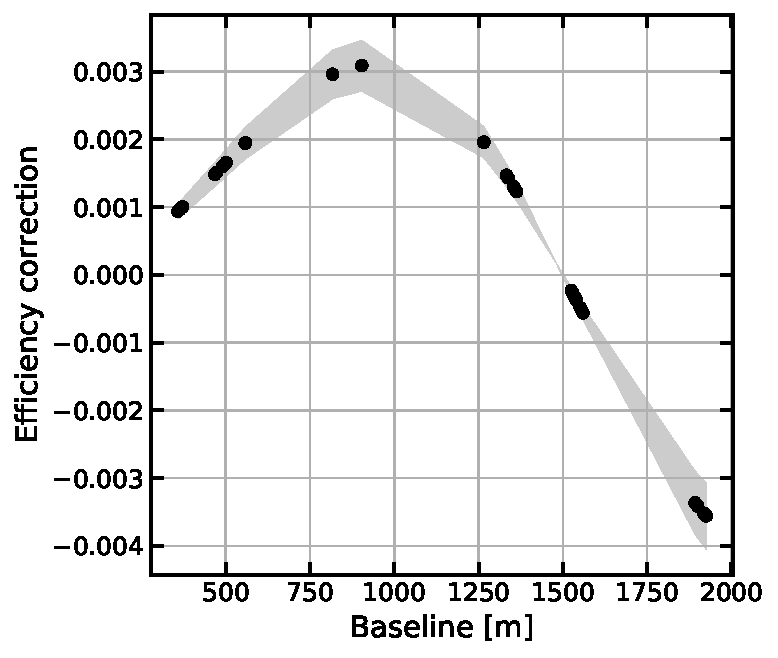
\includegraphics[width=0.5\textwidth]{ch_event_selection/prompt_eff_corrs}
    \caption[Prompt efficiency corrections due to oscillation effects]{
        Corrections to the prompt-energy efficiency due to \nuebar{} oscillations
        ($\delta_{p,ik}$ in the text).
        The data points represent the corrections at the best-fit
        value of \thetaot{} for each AD--reactor pair.
        The shaded band shows the range of corrections when varying \thetaot{}
        over the $\pm1\sigma$ range.
    }
    \label{fig:prompt_eff_osc}
\end{figure}

\begin{figure}
    \centering
    \includegraphics[width=0.49\textwidth]{ch_event_selection/prompt_Eff_corr_EH3_AD1_D1}
    \includegraphics[width=0.49\textwidth]{ch_event_selection/prompt_Eff_corr_EH3_AD1_L1}
    \\
    \includegraphics[width=0.49\textwidth]{ch_event_selection/prompt_Eff_corr_EH1_AD1_D1}
    \caption[Prompt efficiency correction contour maps]{
        Dependence of the prompt-energy efficiency correction
        on the values of the mixing parameters \thetaot{} and $\Delta m^2_{32}$.
        The range for $\sin^22\thetaot{}$ is $\pm2\sigma$ of the best-fit value;
        for $\Delta m^2_{32}$ it is $\pm2\sigma$ of the value reported in \cite{ngd2018}.
        Top left: EH3-AD1 from core D1;
        top right: EH3-AD1 from core L1;
        bottom: EH1-AD1 from core D1.
    }
    \label{fig:prompt_eff_osc_contour}
\end{figure}

The AD-uncorrelated uncertainty for the prompt-energy lower bound
was dominated by differences in the energy scale between ADs.
Based on the analysis of the delayed-energy spectrum in each AD
reported in \cref{subsec:delayed}, the energy scale
varied by less than \SI{0.5}{\percent} between ADs.
By applying a \SI{+-0.5}{\percent} variation to
the reconstructed prompt energy spectrum of the simulated dataset
shown in \cref{fig:prompt_eff_mc} from the Individual Event Simulation,
the impact of the energy scale differences was propagated
to the prompt-energy efficiency.
The impact, and therefore the relative uncertainty on
the prompt-energy efficiency, was \SI{0.1}{\percent}.
This uncertainty was not explicitly included in the
oscillation analysis in \cref{ch:analysis};
rather, it was implicitly derived from the
implementation of the relative energy scale uncertainty.

\subsection{Delayed energy cut efficiency}
\label{subsec:eff_delayed}

The delayed-energy cut efficiency was defined according to \cref{eq:efficiency_def} as
\begin{equation}\label{eq:delayed_eff}
    \varepsilon_\text{delayed} = \frac{N_\text{IBD}[E_p \wedge E_d]}{
        N_\text{IBD}[E_p],
    }
\end{equation}
the fraction of true IBDs passing the prompt-energy selection
which also were accepted by the delayed-energy cuts.
Like for the prompt energy, the absolute efficiency
was measured using the Individual Event Simulation to be approximately \SI{40}{\percent}
but was not used in this analysis.
The primary contribution to the inefficiency
was neutrons capturing on Gd in the GdLS volume;
a subdominant contribution was $\gamma$-rays from nH capture escaping from the LS volume.

\begin{figure}
    \centering
    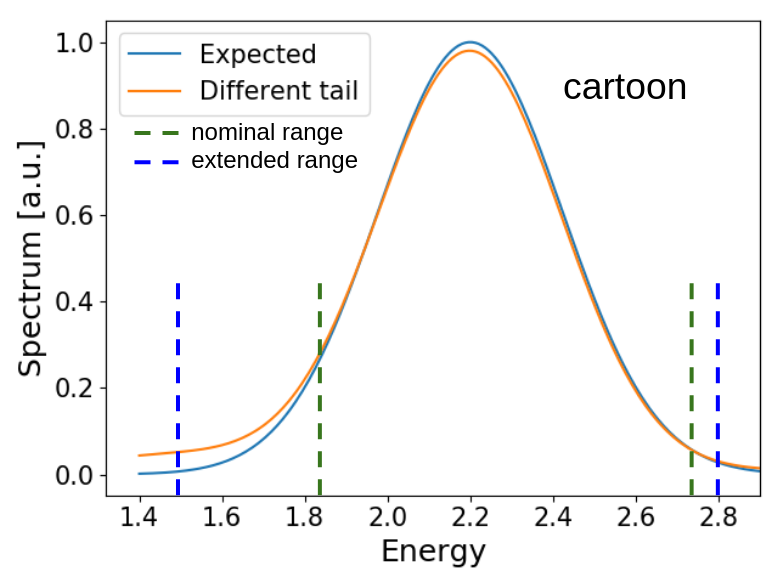
\includegraphics[height=0.4\textheight]{ch_event_selection/delayed_eff_uncertainty_cartoon}
    \caption[Delayed energy efficiency diagram]{
        Depiction of how differences in the relative size
        of the nominal (peak) versus extended ranges
        are a proxy for differences in cut efficiency.
    }
    \label{fig:delayed_eff_unc_cartoon}
\end{figure}

The AD-uncorrelated uncertainty on the delayed-energy cut efficiency
included variations due a wide variety of effects:
geometrical variations, energy scale, different material properties,
Gd fraction, etc.
The overall variation between ADs was estimated using a general method
that compared the relative size between the peak and tail regions
of the delayed-energy spectrum across the ADs.
Intuitively, if the same fraction of events were in the peak region in each AD,
then the cut efficiency must have a small variation.
This intuition is visualized in the diagram in \cref{fig:delayed_eff_unc_cartoon}.
The ``expected'' curve has a higher efficiency
and few events in the tail.
Since the ``different tail'' curve has more events in the tail region,
it can be concluded that this curve has a lower efficiency.
In practice, it was more convenient to compare the number of events in the peak
to the total number of events in an extended region that included the peak and tail,
rather than to just the new events in the tail.

For each AD's delayed-energy spectrum, the peak region was defined as
the region passing the delayed-energy cut, $\vert E_d-\mu \vert < 3\sigma$
(\cref{eq:delayed_cut}), containing $N_\text{peak}$ events.
The extended region, defined by
$\SI{1.5}{\mev} < E_d < \SI{2.8}{\mev}$,
contained $N_\text{extended}$ events.
Using an AD-dependent definition for the peak region but
the same values for the extended region created
the desired sensitivity to variations in the energy scale.
Extending the lower bound down to \SI{1.5}{\mev} added sensitivity to
anything that would change the shape of the tail
or the fraction of $\gamma$'s that (partially or entirely) escape from the AD.

\begin{figure}
    \centering
    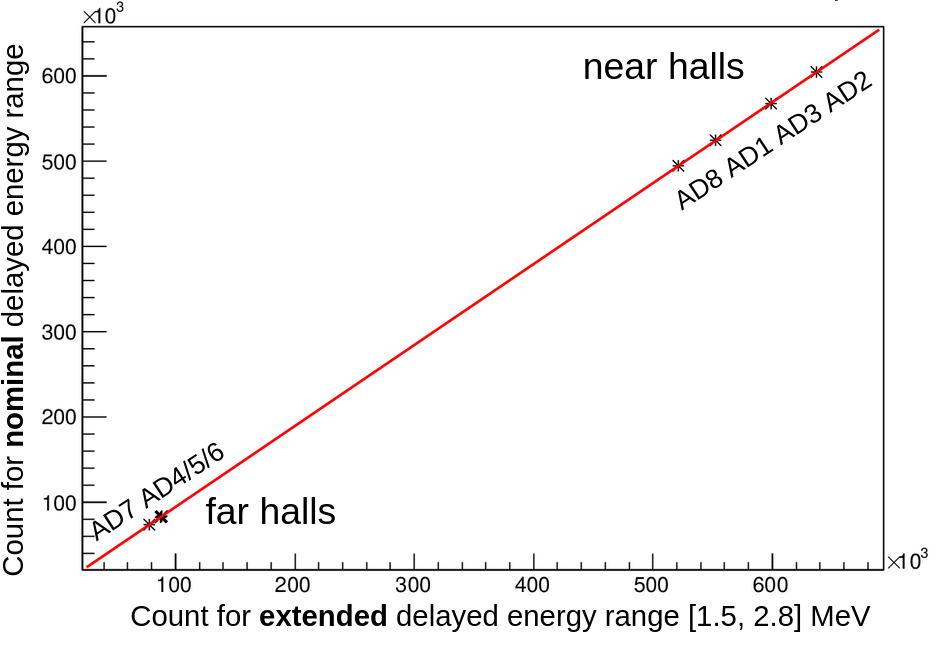
\includegraphics[height=0.4\textheight]{ch_event_selection/delayed_uncertainty_fit}\\
    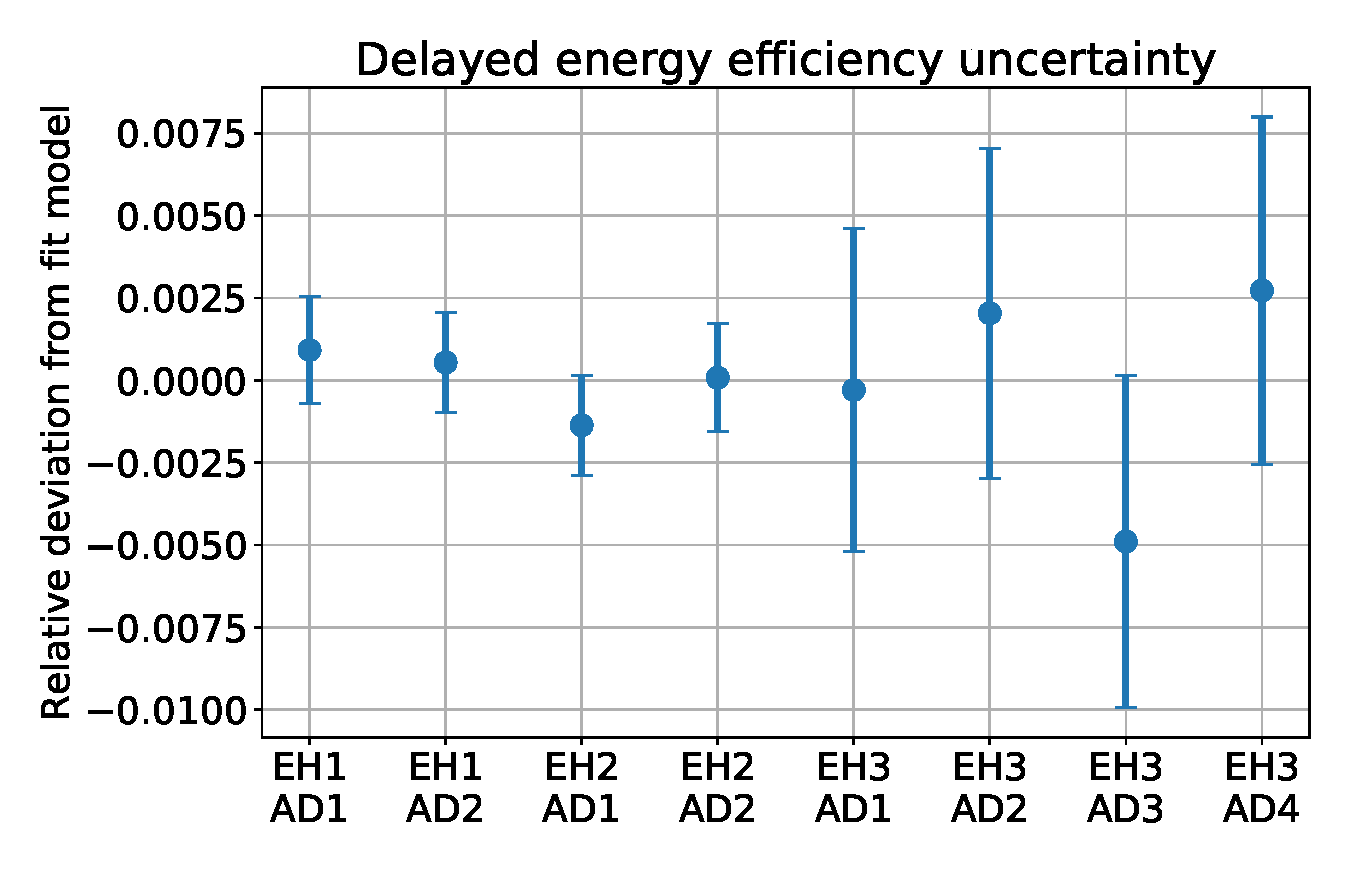
\includegraphics[height=0.4\textheight]{plot_diagnostics/delayed_energy_uncertainty_method1}
    \caption[Delayed energy efficiency uncertainty]{
        (Top) Number of events in the nominal (peak)
        and extended ranges of delayed energy.
        Statistical error bars are too small to be visible on this plot.
        The points are labeled using a shorthand AD indexing scheme:
        ADs 1 and 2 are EH1-AD1 and EH1-AD2. ADs 3 and 8 are EH2-AD1 and EH2-AD2.
        And ADs 4 through 7 are EH3-AD1 through EH3-AD4, respectively.
        The best fit is shown as the red line.\\
        (Bottom) Relative deviations of each hall from the best-fit model.
        The range of deviations for the near-hall ADs
        was used as the delayed-energy efficiency AD-uncorrelated uncertainty.
    }
    \label{fig:delayed_eff_unc_fit}
\end{figure}


If the delayed-energy spectra in each AD have the same shape (same efficiency),
and if the calorimeter function is an appropriate fitting function
for determining the energy cut bounds,
then for some constant $b$ common to all ADs,
$N_{\text{peak},i} = b N_{\text{extended},i}$ for each AD $i$.
To test this model, a linear function was fit
to the values for all ADs:

\begin{equation}
    N_{\text{peak,\,pred},i} = a + b N_{\text{extended},i},
\end{equation}
where $N_{\text{peak,\,pred},i}$ is the fitting function's prediction
of $N_{\text{peak},i}$.
Plots of $N_{\text{peak},i}$ vs. $N_{\text{extended},i}$ and of the
relative deviation from the fitted line are shown in \cref{fig:delayed_eff_unc_fit}.
The fit value of $a$ should be $0$ if the simple model of
a linear scaling is correct.
Indeed, the best-fit value was $a = -323 \pm 387$
which is consistent with $0$.
The best-fit value for $b$ was $b = 0.9527 \pm 0.0015$.

The final value for the AD-uncorrelated uncertainty
of the delayed-energy cut efficiency was taken to be
the range of the relative deviations
of the near-hall ADs from the fitted line: \SI{0.22}{\percent}.
The far-hall ADs had much higher statistical uncertainty
(relative uncertainty \SI{\sim0.5}{\percent}),
and therefore larger fluctuations.
Validation that the far-hall ADs were not
substantially different from the near-hall ADs was obtained by
summing the counts for all 4 far-hall ADs to get
a combined relative deviation for the far hall of \SI{0.018}{\percent},
well within the uncertainty derived from the near halls.

This method for determining the variation in efficiency across ADs
did not account for every possible inefficiency.
For example, if the fraction of $\gamma$-rays that totally
escaped from the scintillating region were different in one AD,
but the distribution of $\gamma$-rays that \textit{partially} escaped were unchanged,
then this method would still suggest a high similarity between ADs.
An assumption of this analysis, therefore, is that any AD-to-AD variation
(in geometry, electronics, scintillator composition, etc.)
that affected the fraction of totally-escaping $\gamma$-rays
also changed the fraction of partially-escaping $\gamma$-rays.

\subsection{Distance-time cut efficiency}
\label{subsec:eff_DT}

Applying the DT cut rejected the vast majority of accidental events
at a loss of approximately \SI{30}{\percent} of real IBDs.
The absolute efficiency was defined as
\begin{equation}\label{eq:abs_DT_eff}
    \varepsilon_{\text{DT}} = \frac{
        N_\text{IBD}[E_p \wedge E_d \wedge \text{DT}]
    }%
    {
        N_\text{IBD}[E_p \wedge E_d]
    },
\end{equation}
the fraction of IBD events passing the prompt- and delayed-energy cuts
that also passed the DT cut.
This value was estimated using a data-driven method
based on the observed distribution of the DT parameter
for all double-coincidence events passing the prompt- and delayed-energy cuts,
with the contribution from the accidental background
statistically subtracted.
Separate 2D histograms $N_\text{obs}$ and $N_\text{acc}'$
were constructed from the observed event sample
and the synthetic accidental background sample (described in \cref{sec:acc}) for each AD,
showing the distribution of the DT parameter and delayed energy.
The $N_\text{acc}'$ histogram was normalized by a factor $k$ so that
the number of events at large DT values
matched the observed number of such accidental coincidences
using the constraint
\begin{equation}\label{eq:acc_sub_normalized}
    \int_{E_d}\int_{\SI{3}{\m}}^{\SI{10}{\m}}
    \frac{d^2N_\text{obs}}{dE_d d(\text{DT})}
    d(\text{DT}) dE_d
    =
    \int_{E_d}\int_{\SI{3}{\m}}^{\SI{10}{\m}}
    k\frac{d^2N_\text{acc}'}{dE_d d(\text{DT})}
    d(\text{DT}) dE_d,
\end{equation}
based on the assumption that all observed events
with a DT parameter greater than \SI{3}{\m}
were accidental coincidences.
The outer integral over delayed energy
used the delayed-energy cut bounds specific to each AD.

\begin{figure}
    \centering
    \includegraphics[width=0.49\textwidth, trim={0 0 0 1cm}, clip]{%
        ch_event_selection/ed_DT_sub_EH1_AD1_normalized%
    }
    \includegraphics[width=0.49\textwidth, trim={0 0 0 1cm}, clip]{%
        ch_event_selection/ed_DT_sub_EH2_AD1_normalized%
    } \\
    \includegraphics[width=0.49\textwidth, trim={0 0 0 1cm}, clip]{%
        ch_event_selection/ed_DT_sub_EH3_AD1_normalized%
    }
    \caption[Delayed energy vs. DT without accidentals]{
        Accidentals-subtracted distribution of
        delayed energy as a function of DT parameter.
        The green (solid) box shows the events included in the DT cut.
        The red (dashed) box shows the events excluded by the DT cut.
        The large fluctuations at high DT are due to the statistics
        of subtracting two almost-equal large numbers as part of the
        background subtraction procedure.
        Histogram bins with negative contents were assigned a value of 1
        to support the logarithmic color scale.
    }
    \label{fig:ed_DT_sub}
\end{figure}

Subtracting the (normalized) $N_\text{acc}'$ histogram from $N_\text{obs}$ bin-by-bin
thus provided the distribution of correlated events
(true IBDs as well as correlated backgrounds)
as a function of delayed energy and DT parameter,
denoted $N_\text{sub}$:
\begin{equation}\label{eq:DT_eff_nsub}
    N_\text{sub} = N_\text{obs} - kN_\text{acc}'.
\end{equation}
The histograms depicting $N_\text{sub}$ for three ADs
are shown in \cref{fig:ed_DT_sub}.
(The others within the same hall were qualitatively identical.)
For these histograms, by construction,
\begin{equation}\label{eq:acc_sub_normalized_zero}
    \int_{E_d}\int_{\SI{3}{\m}}^{\SI{10}{\m}}
    \frac{d^2N_\text{sub}}{dE_d d(\text{DT})}
    d(\text{DT}) dE_d
    = 0.
\end{equation}
A further assumption, that the position distribution of the correlated backgrounds
(most of which involved a prompt event followed by nH capture)
was equal to the position distribution of IBDs,
was made to allow the approximation of \cref{eq:abs_DT_eff} as
\begin{equation}\label{eq:abs_DT_eff_approx}
    \varepsilon_{\text{DT}} \approx \frac{
        N_\text{sub}[E_p \wedge E_d \wedge \text{DT}]
    }%
    {
        N_\text{sub}[E_p \wedge E_d]
    }.
\end{equation}
The statistical uncertainty of the absolute efficiency, $\sigma_\text{DT}$,
was computed assuming $N_\text{sub}[E_p \wedge E_d \wedge \text{DT}]$
followed the binomial distribution:
\begin{equation}\label{eq:abs_DT_eff_uncertainty}
    \sigma_\text{DT} = \sqrt{
        \frac{
            \varepsilon_\text{DT}(1 - \varepsilon_\text{DT})
        }{
            N_\text{sub}[E_p \wedge E_d]
        }
    }.
\end{equation}
The uncertainty due to the accidental background subtraction
was treated as a systematic uncertainty on $\varepsilon_\text{DT}$.

The extracted DT cut absolute efficiency for each AD is shown in
\cref{fig:DT_eff}, top right, with the error bars defined by
\cref{eq:abs_DT_eff_uncertainty}.
Like all absolute detection efficiencies,
$\varepsilon_{\text{DT}}$ was not used as an input to the \thetaot{} analysis.
However, the variation between ADs was treated as the AD-uncorrelated uncertainty
of the DT cut efficiency.
The \SI{>3}{\percent} apparent variation between ADs
was concerning because such a large uncertainty on the overall efficiency
would render a precise measurement of \thetaot{} impossible.
Additional investigation was undertaken to
determine whether the differences in $\varepsilon_\text{DT}$ were intrinsic to the ADs
or were artifacts of the procedure
used to extract the absolute efficiencies.

\begin{figure}
    \centering
    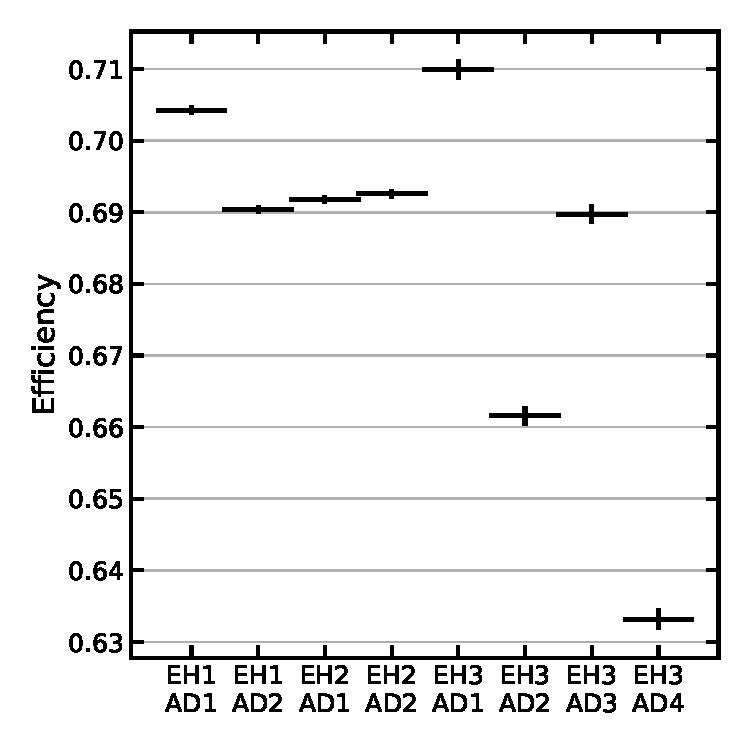
\includegraphics[width=0.49\textwidth]{plot_diagnostics/distance_time_cut_efficiency}
    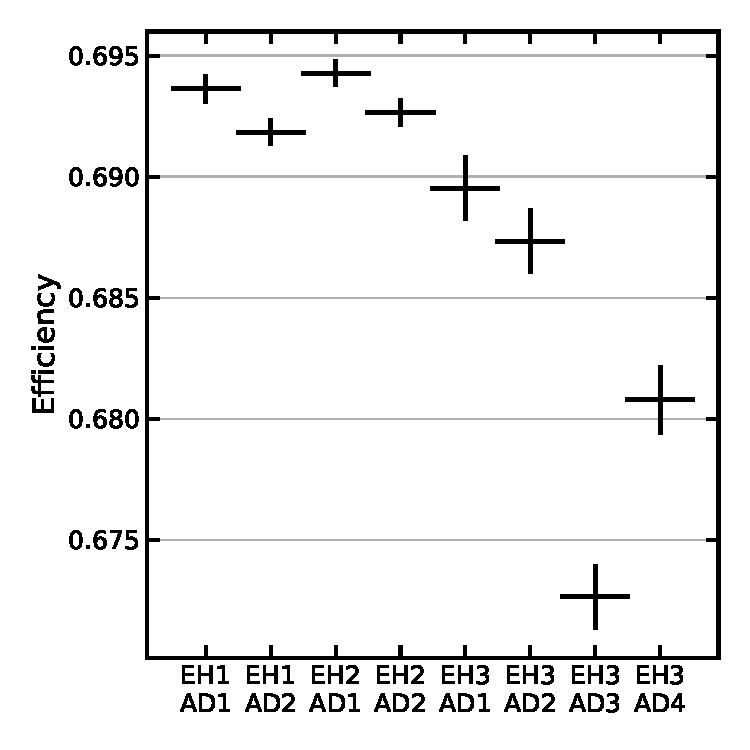
\includegraphics[width=0.49\textwidth]{ch_event_selection/DT_eff_normalized} \\
    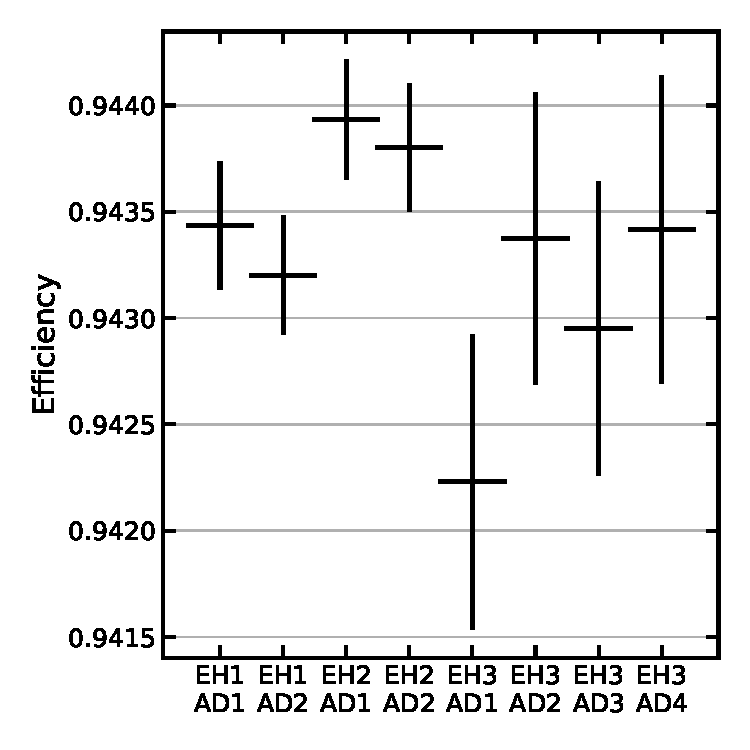
\includegraphics[width=0.49\textwidth]{ch_event_selection/DT_eff_nGd}
    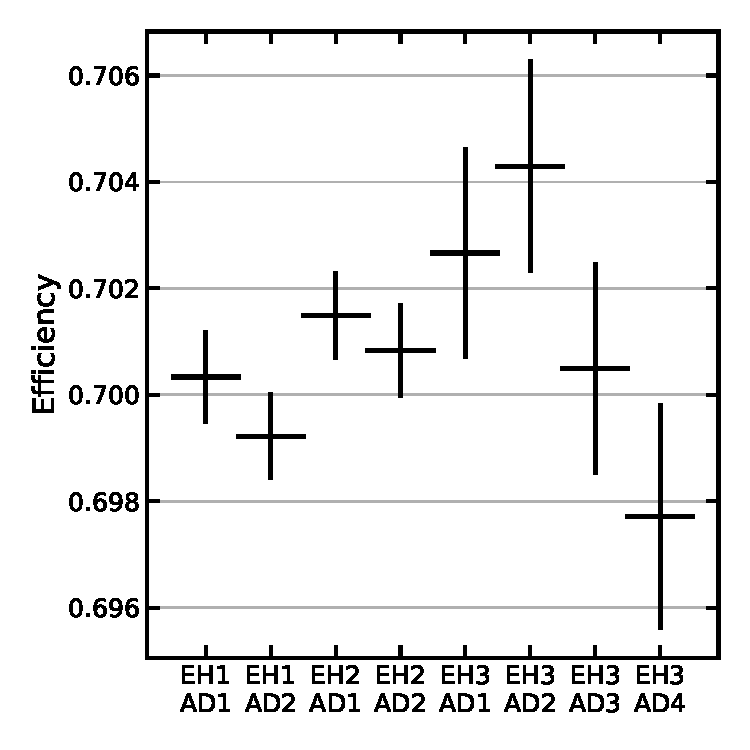
\includegraphics[width=0.49\textwidth]{ch_event_selection/DT_eff_Ep_3.5MeV}
    \caption[DT cut efficiency study]{
        DT cut efficiency for each AD using the four methodologies
        described in the text.
        Top left: singles rate--based subtraction;
        top right: normalized subtraction, nominal energy cuts;
        bottom left: normalized subtraction, nGd capture
        ($\SI{6}{\MeV} < E_d < \SI{12}{\MeV}$);
        bottom right: normalized subtraction, $E_p > \SI{3.5}{\MeV}$.
        The absolute efficiency is not used in the \thetaot{} analysis.
        The AD-uncorrelated uncertainty in the efficiency
        was assigned to be the half-range of the $E_p > \SI{3.5}{\MeV}$
        efficiency measurements, \SI{0.47}{\percent}.
    }
    \label{fig:DT_eff}
\end{figure}

\begin{figure}
    \centering
    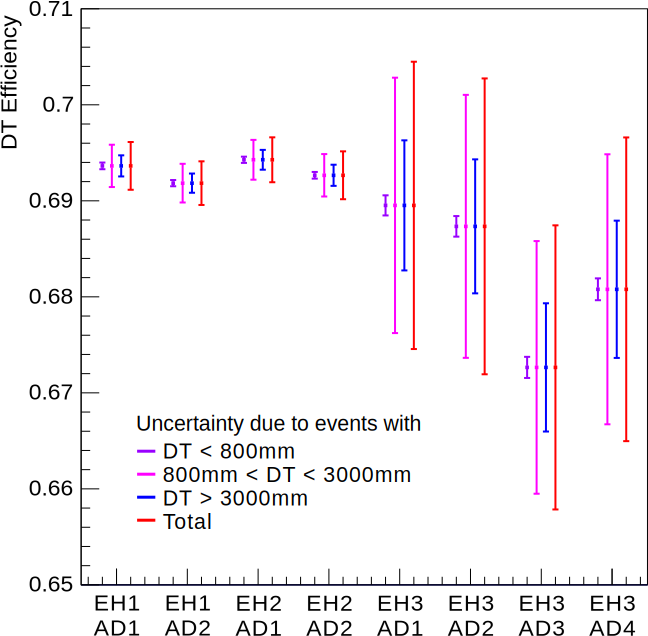
\includegraphics[width=0.5\textwidth]{ch_event_selection/DT_eff_beda}
    \caption[DT efficiency with full statistical uncertainty]{
        DT cut efficiency using the normalized subtraction
        and nominal energy cuts,
        with fully-propagated statistical uncertainties
        from the accidentals subtraction procedure.
        The uncertainties confirm that the apparent AD-to-AD variations
        can be attributed to statistical fluctuations of the accidental background
        rather than intrisic differences between ADs.
        This plot is comparable to the top-right plot of \cref{fig:DT_eff}.
        Figure taken from \cite{beda_DT_eff_unc}.
    }
    \label{fig:DT_eff_beda}
\end{figure}


A more complete model of $\sigma_\text{DT}$ was constructed
to propagate the statistical uncertainties
from $N_\text{obs}$ and $k$ in \cref{eq:acc_sub_normalized}
\cite{beda_DT_eff_unc}.
Using the new model, the apparent \SI{3}{\percent} variation between ADs
observed in the top-right plot of \cref{fig:DT_eff}
was attributable to the statistical uncertainty
of the large number of accidental coincidences within $N_\text{obs}$
which fail the DT cut,
as shown in \cref{fig:DT_eff_beda}.
Even though the fluctuations in
$N_\text{obs}[E_p \wedge E_d \wedge \text{DT} > \SI{3}{\m}]$
due to counting statistics were only \SI{\sim0.03}{\percent},
the absolute efficiency was extremely sensitive to those fluctuations, as follows.

The sensitivity arose in the computation of $N_\text{sub}[E_p \wedge E_d]$.
Most of the range of DT values was characterized by
very few correlated events (signal) but many accidental coincidences (background).
A change of \SI{0.01}{\percent} in $k$, the normalization
of $N_\text{acc}'$ at a far-hall AD,
yielded a relative impact of \SI{2.1}{\percent} in the extracted DT cut efficiency
due to the change in $N_\text{sub}[E_p \wedge E_d]$
from over- or under-subtraction.
Thus any bias in $k$ was amplified into a bias in $\varepsilon_\text{DT}$
over 200 times as large.
The near-hall ADs were sensitive by a factor of ${\sim}30$.

Two special selections were used to reduce the systematic impact of accidental coincidences
on the apparent DT cut efficiency.
The first selection consisted of events where the neutron captured on Gd
rather than H.
They were isolated using the plots shown in \cref{fig:ed_DT_sub}
by selecting the region with delayed energy between \SIlist{6;12}{\MeV}.
The second selection consisted of nH events
with a prompt energy above \SI{3.5}{\MeV}.
The accidentals-subtracted plots of delayed energy versus DT were
regenerated to only include events with $E_p > \SI{3.5}{\MeV}$,
and the DT efficiency procedure was repeated.
The same delayed energy cut was used for this modified sample
as for the nominal sample.
The nGd subset yielded a full range of \SI{0.18}{\percent}
in DT cut absolute efficiencies over all ADs,
while the $E_p > \SI{3.5}{\MeV}$ yielded a full range of \SI{0.94}{\percent}.
The extracted efficiencies for each AD are shown in
the bottom row of \cref{fig:DT_eff};
the error bars on each AD now indicate the values are consistent across ADs
even without accounting for the uncertainty in the accidentals subtraction.
Between these two subsets, almost the entire range
of prompt and delayed positions and energies used in the nominal selection was represented,
as shown in \cref{fig:DT_energy_range}.
Thus the DT cut efficiency uncertainty was accurately estimated
with a minimal impact from the accidental background.
Conservatively, the half-range of the $E_p > \SI{3.5}{\MeV}$ subset,
\SI{\pm0.47}{\percent}, was
used as the AD-uncorrelated uncertainty of the DT cut efficiency.

\begin{figure}
    \centering
    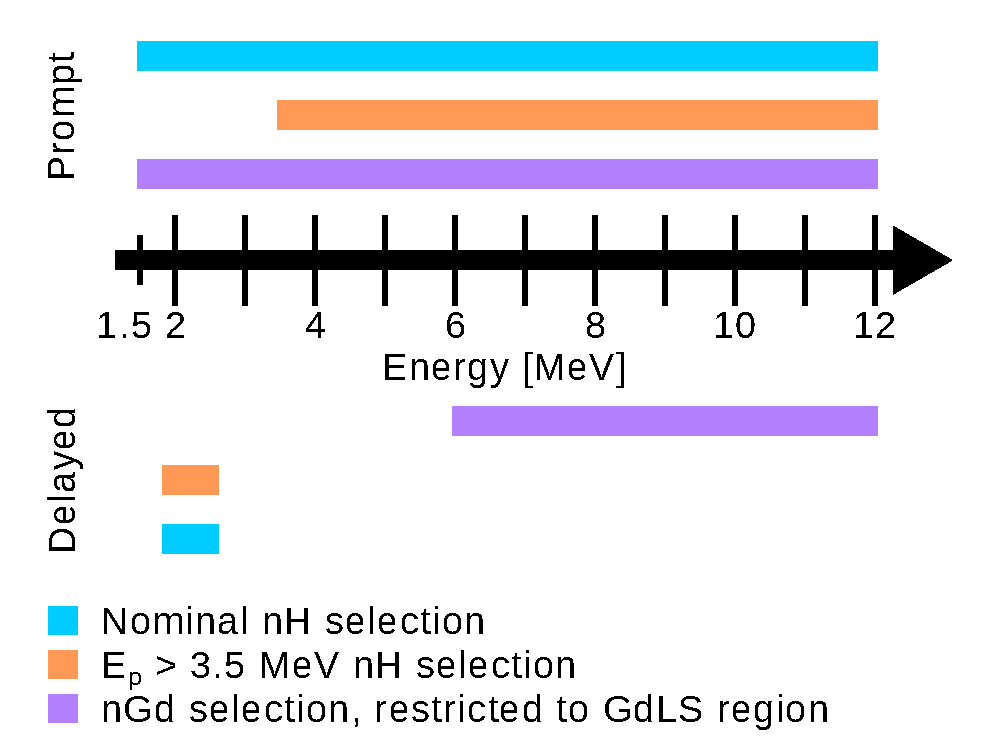
\includegraphics[width=0.6\textwidth]{ch_event_selection/DT_eff_energy_coverage}
    \caption[DT efficiency study energy coverage]{
        Energy ranges for the three selections used to constrain
        the AD-uncorrelated uncertainty of the DT cut efficiency.
        Combined, the two special selections cover the entire range of event energy
        and almost the entire range of event positions
        present in the full nominal nH selection.
    }
    \label{fig:DT_energy_range}
\end{figure}

The normalization factors derived for each AD ($k$ in \cref{eq:acc_sub_normalized})
corresponded to an effective accidental coincidence rate
within \SI{\pm0.04}{\percent} of the rate computed
using the nominal singles rate--based methodology from \cref{sec:acc}---%
a serendipitous validation of the low systematic bias
in the accidental background rates.
The top-left panel of \cref{fig:DT_eff} shows an attempt
at measuring the DT cut efficiency by setting $k$ based on \cref{eq:nacc}
rather than \cref{eq:acc_sub_normalized};
the discrepancy of ${\sim}0.06$ between EH3-AD4's efficiency and the near-hall average
is consistent with the expected impact
of the normalization error of \SI{0.04}{\percent} listed in \cref{tab:acc_validation}.
Thus although the nominal, rate-based methodology
for determining the normalization of $N_\text{acc}'$
was precise enough
for computing \thetaot{},
it was not precise enough for computing the DT cut efficiency.

\section{Irreducible correlated backgrounds}
\label{sec:correlated_bg}

Any event in the double coincidence dataset
that passed all multiplicity, distance, and energy cuts
and that was not caused by an IBD interaction followed by
neutron capture on hydrogen (nH)
was an irreducible background.
The accidental background analysis (\cref{sec:acc})
characterized the rate and spectrum of
the irreducible uncorrelated background,
but it was not sensitive to physical processes that produced
correlated prompt-delayed pairs.
These correlated backgrounds included muon-induced unstable isotopes (\cref{subsec:li9}),
muon-induced fast neutrons (\cref{subsec:fastn}),
$\gamma$-rays from the \amc{} calibration source (\cref{subsec:amc}),
and radiogenic neutrons (\cref{subsec:radn}).

\subsection{Muon-induced unstable isotopes}
\label{subsec:li9}

\begin{figure}
    \centering
    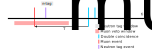
\includegraphics{ch_event_selection/timeline_li9}
    \caption[\li{}/\he{} event selection]{
        Event selection procedure for \li{} events.
        Neutron tags were identified within a short time window
        immediately following the muon.
        The time delay between the prompt event and the muon
        was stored in a time-to-previous-muon histogram.
        The muon veto window was ignored.
    }
    \label{fig:li9_timeline}
\end{figure}

Muon interactions with nuclei (primarily \isotope[12]{C}) in the AD
produced the unstable exotic isotopes \li{} and \he{}.
These isotopes $\beta$-decayed to neutron-unstable excited states
of \isotope[9]{Be} and \isotope[8]{Li}, respectively,
leading to a nonzero probability of a $\beta^{-}$-n coincidence \cite{kamland_li9}.
Unfortunately, the range of $\beta^-$ energies overlapped substantially
with the range of IBD prompt ($e^+$) energies,
and neutrons from $\beta^-$-n decays behaved
exactly the same as neutrons from IBD interactions.
Thus the \li{} and \he{} decays had the same signature as true IBDs.
Further, the lifetimes for \li{} and \he{} were
\SI{257.23}{\ms} and \SI{171.60}{\ms}, respectively,
meaning that the \SI{800}{\us} veto for AD muons
with energy below \SI{2.5}{\GeV} will almost always
\emph{not} veto the subsequent \li{} or \he{} decay.
The shower muon veto of \SI{1}{\s} still allowed acceptance of
${\sim}e^{-4}$ of the associated \li{} and \he{} events.
In the following, unless otherwise stated,
\li{} will be used to mean both \li{} and \he{}.

The number of \li{} events contaminating the double coincidence sample
was determined by exploiting those events' time correlation
with the muon event that created the parent \li{} nucleus \cite{jinjing_2020may}.
An alternate event selection with no post-muon veto
was performed to increase the contribution of \li{} events
in the resulting data sample.
Additionally, the prompt-energy threshold
was raised to $E_p > \SI{3.5}{\MeV}$
to reduce the impact of accidental events.
Muon events were categorized into energy classes
of \SIrange{0.02}{1}{\GeV}, \SIrange{1}{2.5}{\GeV},
and \SI{>2.5}{\GeV}.
Additionally, any muon that was accompanied by
an AD event with energy between \SIlist{1.8;12}{\MeV}
during the interval of \SIrange{20}{200}{\us} following the muon
was ``tagged'' as a neutron-producing muon.
These neutron-tagged muons had an increased likelihood
of producing \li{}.
For each energy class of muon,
an additional subsample of neutron-tagged muons was also formed.

The double coincidence candidates which passed the alternate selection
were categorized based on the classification
of the most recent preceding AD muon,
and the time since the preceding muon
was saved in a histogram specific to the muon class.
Since the \li{} process was common to all of the ADs within a given hall,
the events from ADs in the same hall were combined
to improve the statistical uncertainty of the rate estimation.
A visualization of the alternate event selection
is shown in \cref{fig:li9_timeline};
a summary of the selection criteria is listed in \cref{tab:li9}.

The distribution of times since the preceding muon
for events correlated with muons (namely \li{})
was different from the distribution for events uncorrelated with muons
(such as IBDs or accidental backgrounds).
In particular, for muon-uncorrelated events,
the probability density for time since the preceding muon
being between $t$ and $t + dt$ was \cite{chris_li9}
\begin{equation}\label{eq:li9_muon_uncorr}
    p_\text{uncorr}(t) = R_\mu e^{-R_\mu t}dt,
\end{equation}
where $R_\mu$ was the rate of muon events in the particular category being examined.
Muon-correlated events had a time-since-muon distribution
that depends on both the muon rate and the decay lifetime:
\begin{equation}\label{eq:li9_muon_corr}
    p_\text{corr}(t) = \lambda_\text{iso} e^{-\lambda_\text{iso} t}dt,
\end{equation}
where $\lambda_\text{iso} = R_\mu + 1/\tau_\text{iso}$
and $\tau_\text{iso}$ is the decay time
for the muon-correlated isotope.

\begin{table}[ht]
    \centering
    \caption[\li{}/\he{} event selection]{Modified event selection for \li{} analysis.}
    \label{tab:li9}
    \begin{tabular}[t]{rl}
        \toprule
        Post-muon veto & No veto after shower muons \\
        Prompt energy cut & \SI{3.5}{\MeV} \\
        Delayed energy cut & see \cref{tab:delayed_bounds} \\
        Low-energy muon range & \SIrange{0.02}{1}{\GeV} \\
        Mid-energy muon range & \SIrange{1}{2.5}{\GeV} \\
        High-energy muon range & \SI{>2.5}{\GeV} \\
        Neutron tag event time & \SIrange{20}{200}{\us} after muon \\
        Neutron tag event energy & \SIrange{1.8}{12}{\MeV} \\
        \bottomrule
    \end{tabular}
\end{table}

At very short times since the preceding muon,
there was an additional muon-correlated signal
which, unlike \li{}, did decay away completely
during the nominal muon veto windows.
This signal consisted of accidental coincidences
of two \boron{} decays,
which were known to be produced in large quantities
during muon events \cite{kamland_li9}
and had a lifetime of \SI{20.2}{\ms}.
The distribution of time since the preceding muon
for \boron{}-\boron{} accidental coincidences
had the same form as \cref{eq:li9_muon_corr},
except that $\lambda_\text{B} = R_\mu + 2/\tau_{B}$
since two \boron{} decays are required.

The measured distributions of times since the preceding muon
were each fit independently with a linear combination of the above distributions:
\begin{align}\label{eq:li9_fit_fn}
    \begin{split}
        f(t) &= N_\text{bkg} \left[r \lambda_\text{Li} e^{-\lambda_\text{Li} t}
        + (1-r) \lambda_\text{He} e^{-\lambda_\text{He} t}\right] \\
             &+ N_\text{uncorr} R_\mu e^{-R_\mu t} \\
             &+ N_\text{B} \lambda_\text{B} e^{-\lambda_\text{B} t}
    \end{split}
\end{align}
In this fit, $N_\text{bkg}, N_\text{uncorr}$, and $N_\text{B}$
were free parameters representing the number of \li{} events,
number of muon-uncorrelated events (IBDs and other backgrounds),
and \boron{}-\boron{} coincidences, respectively.
The fits were not sensitive enough to extract $r$,
the fraction of the background due to \li{} rather than \he{},
so the value of $r$ was fixed at 0.9 during the fit procedure.
A systematic uncertainty was assessed by manually varying $r$
between 0.85 and 1.0
and observing the impact on $N_\text{bkg}$ \cite{li9_details}.
The histograms and best-fit curves for EH1 and EH3 are shown
in \cref{fig:li9_fits_EH1,fig:li9_fits_EH3} \cite{jinjing_2020may}.
The histograms for EH2 are qualitatively the same as those for EH1.

\begin{figure}
    \centering
    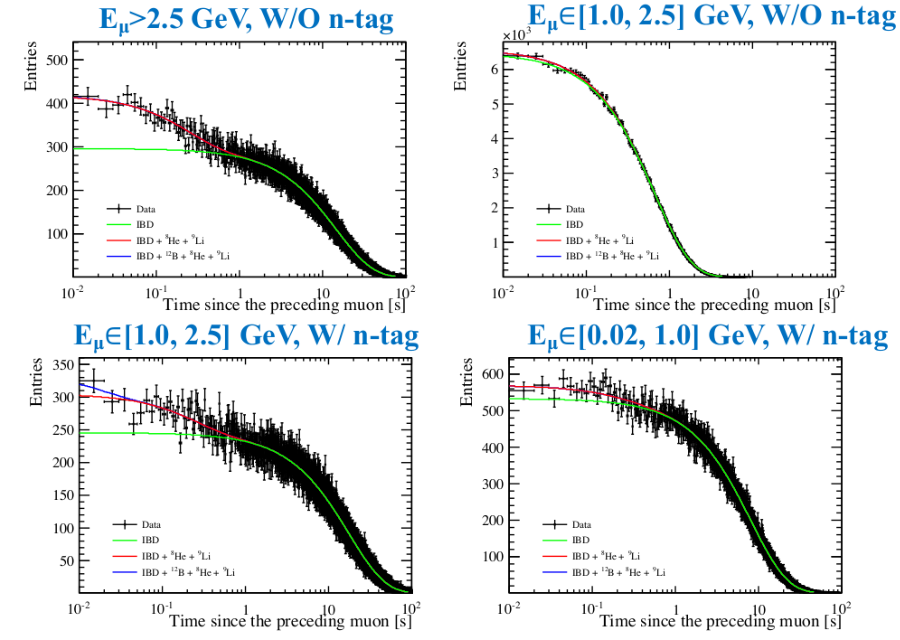
\includegraphics{ch_event_selection/li9_fit_plots_EH1}
    \caption[Time-since-muon histograms for EH1]{
        Histograms of time since the preceding muon at EH1.
        The histograms for EH2 are qualitatively the same as for EH1.
        Taken from \cite{jinjing_2020may}.
    }
    \label{fig:li9_fits_EH1}
\end{figure}

\begin{figure}
    \centering
    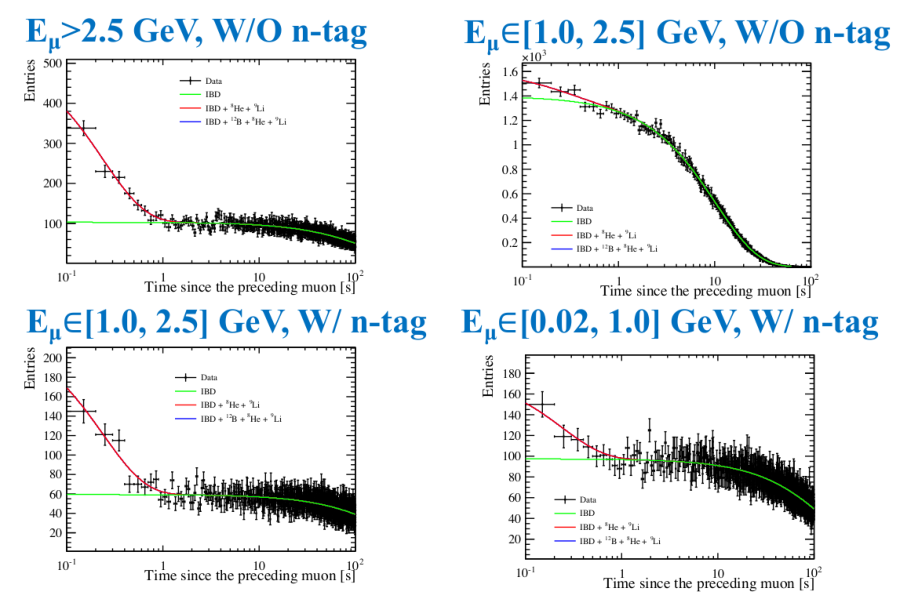
\includegraphics{ch_event_selection/li9_fit_plots_EH3}
    \caption[Time-since-muon histograms for EH3]{
        Histograms of time since the preceding muon at EH3.
        Taken from \cite{jinjing_2020may}.
    }
    \label{fig:li9_fits_EH3}
\end{figure}

For the lowest energy class (\SIrange{0.02}{1}{\GeV}),
production of \li{} was so rare that the fitter
could not effectively discriminate the \li{} events
on top of the muon-uncorrelated events (i.e. IBDs and accidentals).
Thus only the neutron-tagged sample was used to characterize this muon sample.
A systematic uncertainty of \SI{100}{\percent} was assessed
on the neutron tag efficiency $\varepsilon_{ntag}$,
the estimated fraction of \li{} events produced by neutron-tagged muons.
The value of this efficiency was estimated by examining
the corresponding efficiency for the middle energy class of muons,
where it had a value of \SI{83}{\percent}, \SI{42}{\percent}, and \SI{72}{\percent}
in EH1, EH2, and EH3, respectively.

The extracted values for $N_\text{bkg}$ for each class of muons
were converted into the number of \li{} events
actually contaminating the neutrino candidate data sample
using the following formula:
\begin{equation}\label{eq:li9_rate_conv}
    N_\text{in data}^{\text{AD }i} =
    \frac{\varepsilon_p(\SI{1.5}{\MeV})}{\varepsilon_p(\SI{3.5}{\MeV})}
    \times
    \frac{\varepsilon_{\mu,i} T_{\text{DAQ},i}}{
        \sum_j \varepsilon_{\mu,j} T_{\text{DAQ},j}
    }
    \times
    \sum_{E\in\set{E_1,E_2,E_3}}
    \frac{N_{\text{bkg},E}}{\alpha_{ntag, E}} e^{-V_E/\tau_{\text{Li}}}.
\end{equation}
The first term corrected for the different prompt-energy cut
in the \li{} selection compared to the nominal IBD selection;
the efficiencies were based on the \li{} prompt spectrum computed below
and were approximately \SI{80}{\percent}.
The second term divided the events within an entire hall
into portions attributed to each AD based on the nominal unvetoed livetime.
The index $j$ sums over all ADs within the same hall.
The third term is a sum of the extracted event counts
over the three muon energy classes, denoted by $E_1,E_2,E_3$.
The weighting factor $\alpha_{ntag,E}$ accounted
for the use of the neutron-tagged sample for class $E_1$
and was defined as:
\begin{align}
    \begin{split}
        \alpha_{ntag,E1} &= \varepsilon_{ntag,E2} \\
        \alpha_{ntag,E2} = \alpha_{ntag,E3} &= 1,
    \end{split}
\end{align}
where $\varepsilon_{ntag,E2}$ is the neutron tag efficiency defined earlier.
The exponential factor accounted for \li{} decay
over the actual muon veto windows in the nominal event selection,
which had values $V_{E1} = V_{E2} = \SI{800}{\us}$
and $V_{E3} = \SI{1}{\s}$.

\begin{figure}
    \centering
    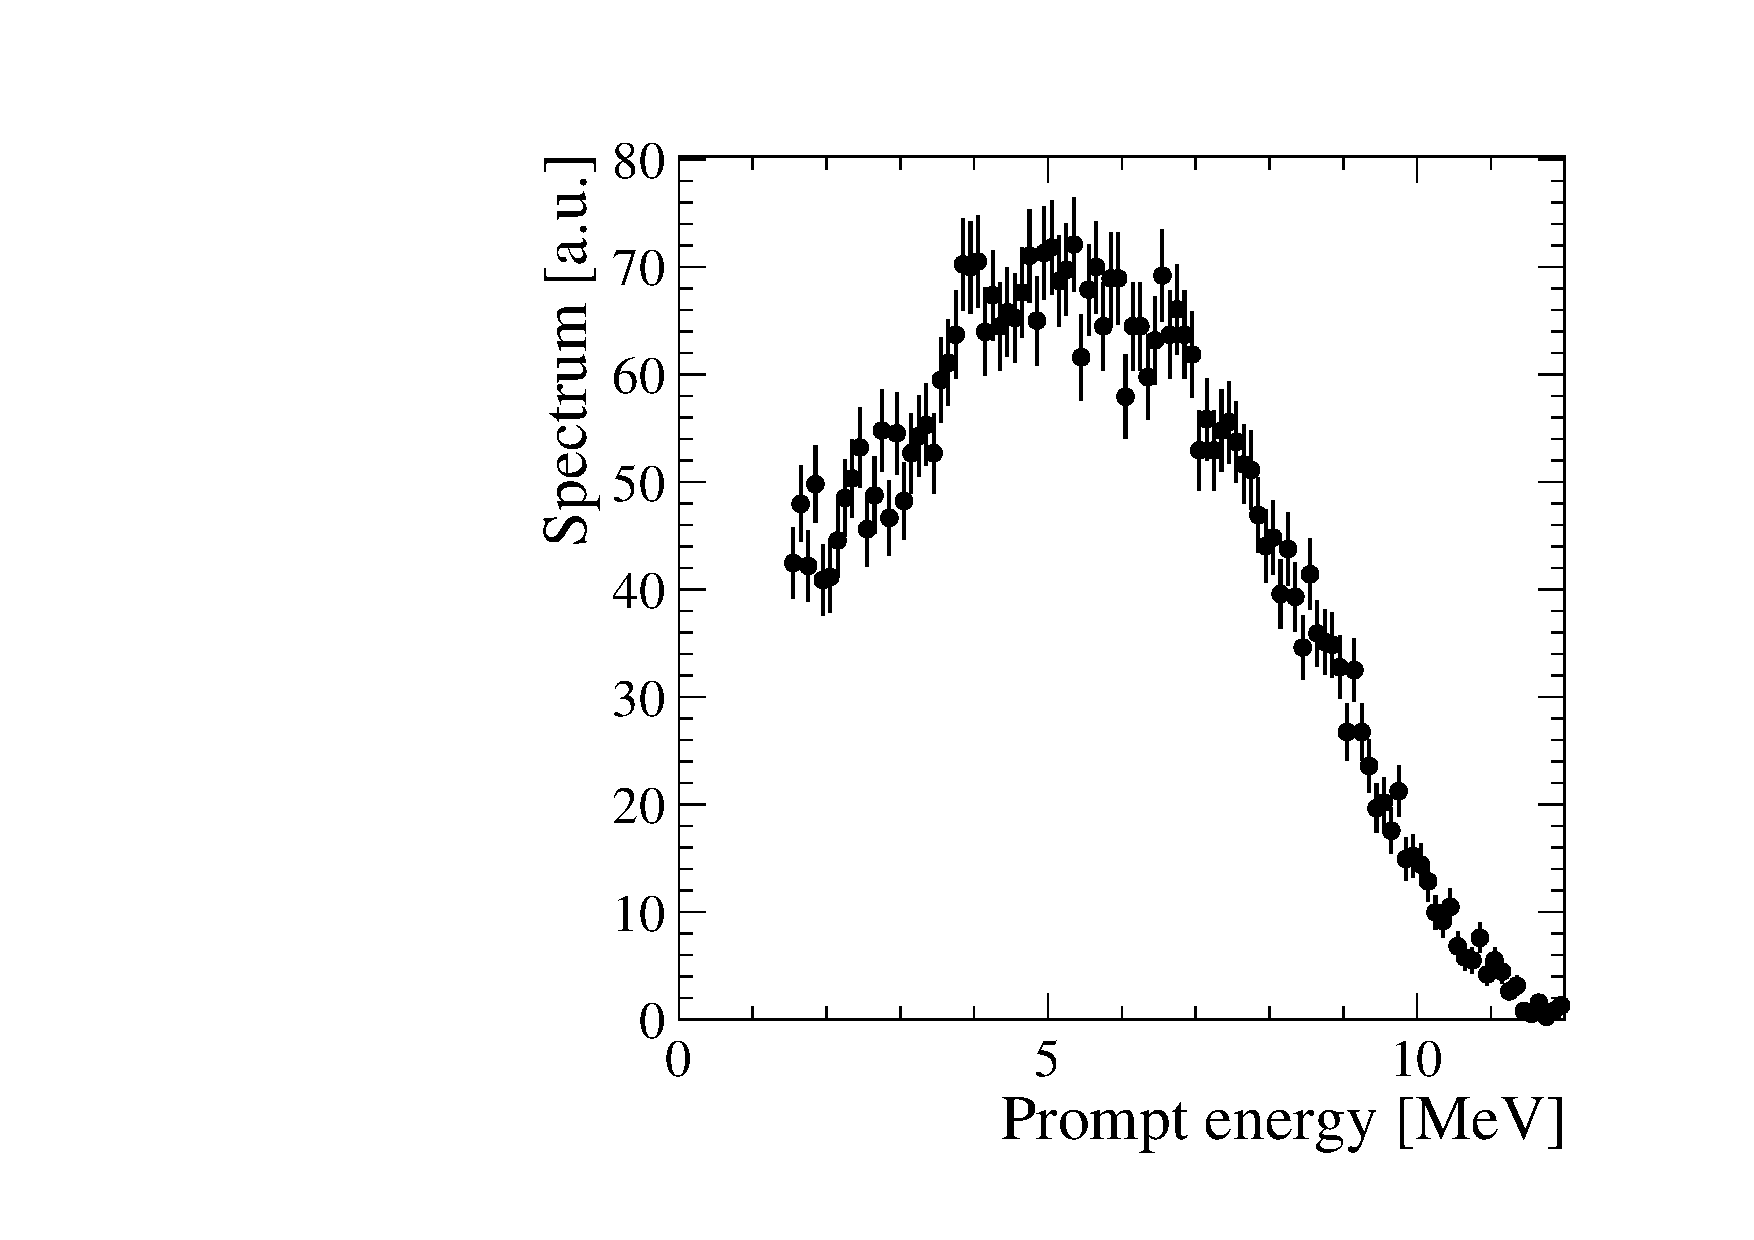
\includegraphics[width=0.5\textwidth]{ch_event_selection/li9_spectrum}
    \caption{
        Prompt-energy spectrum of \li{} background events.
    }
    \label{fig:li9_spec}
\end{figure}

The energy spectrum of the \li{} events was computed
by comparing a \li{}-rich sample to a pure-IBD sample of events
obtained by extending the shower muon veto.
The prompt spectrum from the pure-IBD sample
was normalized to the fitted value for $N_\text{uncorr}$
and subtracted from the prompt spectrom of the \li{}-rich sample.
The resulting \li{} prompt spectrum is shown in \cref{fig:li9_spec}
and was assumed to be common among all ADs.
The prompt energy cut efficiency ratio
used to estimate the actual contamination in the IBD candidate sample
was computed based on this spectrum.

The sources of uncertainty in the number of \li{} events
in the double-coincidence data sample
can be seen in the quantities that contributed to \cref{eq:li9_rate_conv}.
The prompt-energy cut efficiency ratio has an uncertainty
due to the statistical uncertainty of each bin in the extracted \li{} spectrum
(\cref{fig:li9_spec}).
No uncertainty was attributed to the livetime factor since
both the livetime and muon veto efficiency were known precisely.
The neutron tag efficiency
was the dominant source of systematic uncertainty,
comprising nearly all of the quoted uncertainty in \cref{tab:summary_event_selection}.
Other sources of uncertainty considered were
the statistical error from the fit to extract $N_\text{bkg}$,
the uncertainty of the \SI{3.5}{\MeV} prompt energy cut efficiency,
and the uncertainty of the \li{} to \he{} ratio $r$.

\subsection{Muon-induced fast neutrons}
\label{subsec:fastn}

Muon interactions in the rock surrounding the Daya Bay experimental halls
could produce energetic ``fast'' neutrons
which occasionally penetrated through the water pools
and into the scintillating volume in an AD.
These fast neutrons could scatter off a proton in the scintillator,
with the proton recoil causing a prompt-like scintillation signal.
When the neutron subsequently captured on a hydrogen or gadolinium nucleus,
the resulting prompt-delayed coincidence
could pass all selection criteria and contaminate the double-coincidence data set.

\begin{figure}
    \centering
    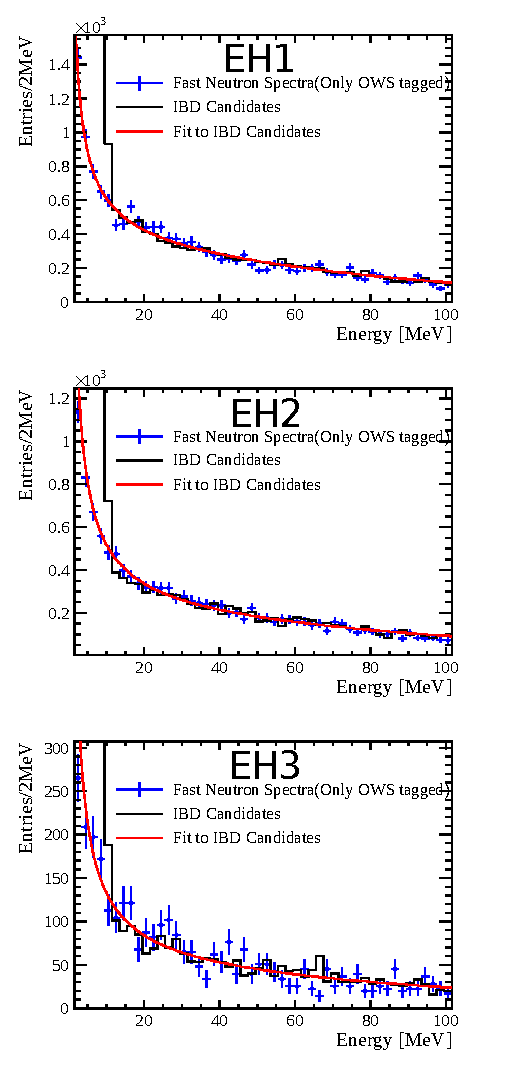
\includegraphics[height=0.8\textheight]{ch_event_selection/fast_neutron_spectra}
    \caption[Fast neutron spectrum]{
        Prompt-energy spectra for each hall
        showing the extended double coincidences (``IBD candidates'')
        and the OWS-tagged sample used to compute the fast neutron background.
        The OWS-tagged sample has been normalized
        so that its integral from \SIrange{12}{300}{\MeV}
        matches the same integral in the extended double coincidence sample.
        The red curve is a fit of \cref{eq:fast_neutron_powerlaw}
        to the double-coincidence sample over \SIrange{12}{300}{\MeV}
        and has been extrapolated to the lower-energy (nominal) range.
    }
    \label{fig:fast_neutron}
\end{figure}

The presence of fast-neutron events in the double-coincidence data set
was demonstrated by modifying the event selection
to remove the upper limit on prompt energy (nominally $E_p < \SI{12}{\MeV}$)
and examining events with prompt energy up to \SI{300}{\MeV}
(keeping all other event selection criteria intact),
as shown in in \cref{fig:fast_neutron}.
The long tail of the spectrum was attributed to fast-neutron events.
This tail provided an important constraint on the fast-neutron contamination
in the nominal double-coincidence data set.
The modified data set will be referred to as the
``extended double-coincidence'' data set.

\begin{table}[ht]
    \centering
    \caption[OWS tag criteria]{
        Modified event selection criteria for the OWS-tagged
        double-coincidence sample.
    }
    \label{tab:fast_neutron}
    \begin{tabular}[t]{rl}
        \toprule
        Quantity & Selection criterion \\
        \midrule
        Prompt energy & \SIrange{1.5}{301.5}{\MeV} \\
        Delayed energy & see \cref{tab:delayed_bounds} \\
        Time from OWS muon to prompt signal & \SI{<0.3}{\us} \\
        Time from any other muon to prompt signal & \SI{>1200}{\us} \\
        \bottomrule
    \end{tabular}
\end{table}


The number of such fast-neutron events in the nominal double-coincidence data set
was estimated by isolating a sample of fast-neutron events
tagged by the muon system.
The resulting spectrum could be normalized based on the high-energy tail
of the modified sample's prompt-energy spectrum
to provide a prediction of the rate and spectrum of fast-neutron events
with lower energies.

The fast-neutron events were selected by searching for
double coincidences associated with signals
in the outer water shield (OWS) of the muon system
which had no other associated muon signal
(see \cref{tab:fast_neutron}).
These events were assumed to be fast-neutron events
which were caused by muons that traversed the outer water shield.
The veto for all other muons was still applied in this sample,
particularly the inner water shield (IWS) veto,
so that there was no ambiguity about whether an AD signal
was a muon or an energetic proton recoil from a fast neutron.
The OWS-tagged sample and the extended double coincidence sample for each hall
are shown in \cref{fig:fast_neutron}.
To extract the number of fast neutron events in the double coincidence sample,
the OWS-tagged sample was scaled by the normalization factor
\begin{equation}\label{eq:fast_neutron_integral}
    k_\text{fast neutron} = \frac{
        \int_{\SI{12}{\MeV}}^{\SI{300}{\MeV}} \frac{dN_{\text{extended}}}{dE} dE
    }{
        \int_{\SI{12}{\MeV}}^{\SI{300}{\MeV}} \frac{dN_{\text{OWS}}}{dE} dE
    },
\end{equation}
where the ``extended'' term refers to the histogram of prompt energies
of the extended double coincidence sample,
and the ``OWS'' term refers to the histogram for the OWS-tagged sample.
The integral notation is used for simplicity,
but in practice the bins are summed over as $\sum_i N(E_i)$.
As shown in \cref{fig:fast_neutron},
there is very good agreement in the shape of the two spectra.
The number of fast neutrons in the nominal double-coincidence sample
is estimated as the number of events in the normalized OWS-tagged histogram
over the nominal prompt energy range of \SIrange{1.5}{12}{\MeV}:
\begin{equation}\label{eq:fast_neutron_count}
    N_\text{fast neutron} = k_\text{fast neutron}
    \int_{\SI{1.5}{\MeV}}^{\SI{12}{\MeV}} \frac{dN_{\text{OWS}}}{dE} dE.
\end{equation}

The uncertainty in this estimate was computed from three sources
based on a parametri\-zation of the shape of the OWS-tagged spectrum
using a modified power law function:
\begin{equation}\label{eq:fast_neutron_powerlaw}
    \frac{dN}{dE} = N_0 \left(\frac{E}{E_0}\right)^{-a-\frac{E}{E_0}},
\end{equation}
where $N_0,a$, and $E_0$ are free parameters.
This function was fit to the extended double-coincidence spectrum
over the energy range \SIrange{12}{300}{\MeV}
and extrapolated to the lower-energy region,
as shown in \cref{fig:fast_neutron}.
The uncertainties were derived based on the fitted function's
ability to predict the value of $N_{\text{fast neutron}}$
computed in \cref{eq:fast_neutron_count}
by integrating the fitted function to obtain $N'_\text{fast neutron}$
The three sources of uncertainty were as follows:
(1) the full range of resulting $N'$ values
when fit was performed using bin widths of \SIlist{1;2;3;4}{\MeV};
(2) the maximum value of $\vert N_\text{fast neutron} - N'_\text{fast neutron}\vert$
over the different binnings;
and (3) the uncertainty in $N'_\text{fast neutron}$ due to
the propagation of the parameter errors from the fit.
For (3), the specific bin width used was arbitrarily chosen to be \SI{2}{\MeV}.
The value $N_\text{fast neutron}$ by construction did not depend
on the modified power law function in \cref{eq:fast_neutron_powerlaw}
or the binning used to perform the fit.

\subsection{\texorpdfstring{\amcbold}{Am-C} calibration source}
\label{subsec:amc}

\begin{figure}
    \centering
    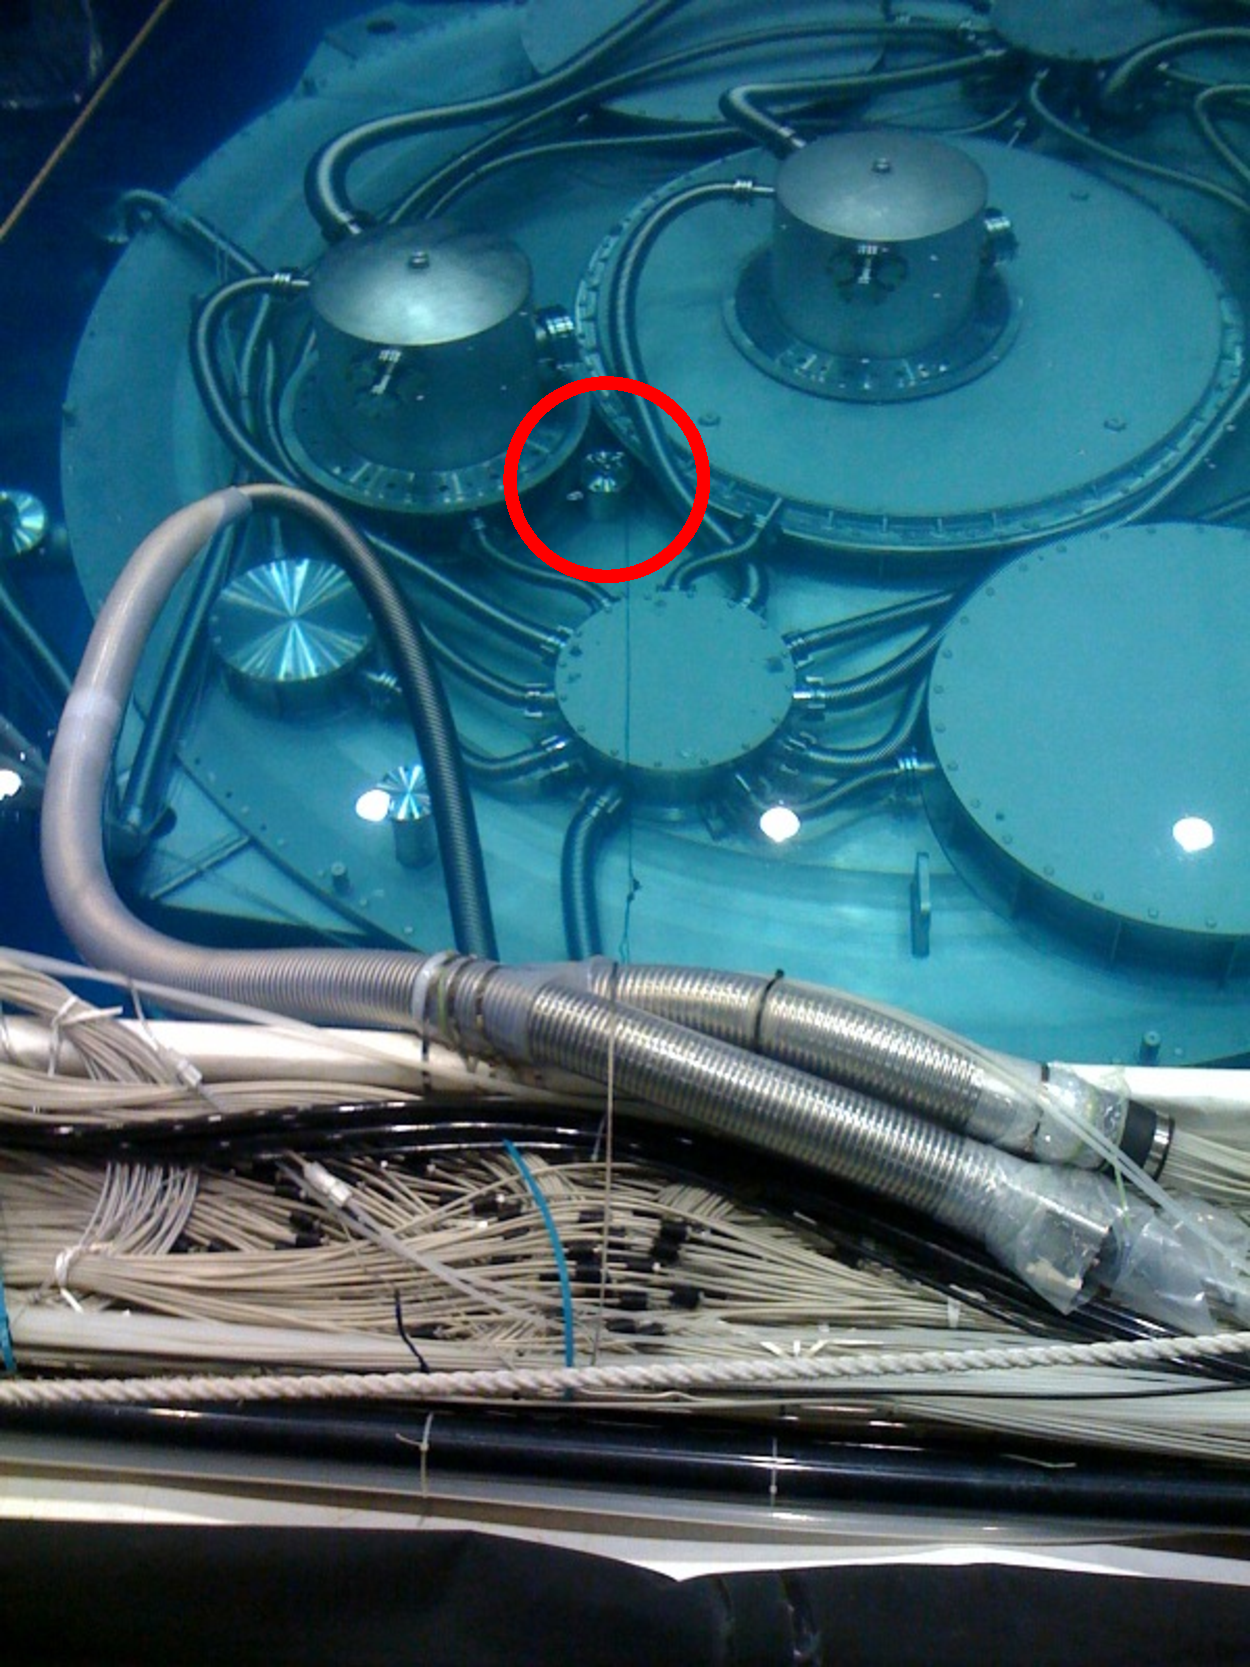
\includegraphics[width=0.5\textwidth]{ch_event_selection/amc_photo_circled}
    \caption[Intense \amc{} source photograph]{
        Photograph of the intense \amc{} source (circled in red)
        on the lid of EH3-AD2 between ACU-B and ACU-C \cite{amc_photo}.
    }
    \label{fig:amc_photo}
\end{figure}

The \amc{} calibration sources emitted neutrons at a rate of \SI{\sim0.7}{\Hz}
to allow for calibration of the ADs' response to neutron-capture events
(\cref{ch:calibration}).
When not deployed during weekly calibrations, these sources
were stored within the ACUs at the top of each AD.
The sources were designed to minimize
the potential for correlated signals to reach the scintillating volume,
e.g. by attenuating the $\alpha$ energy below the $\gamma$ production
threshold for interactions with \isotope[13]{C} \cite{ngd2016}.
However, the emitted neutrons were still able to generate
correlated signals as follows.
The prompt event consisted of an emitted neutron colliding inelastically
with a nucleus (Fe, Cr, Mn or Ni) in the stainless steel surrounding the AD and ACU,
producing $\gamma$-rays one of which occasionally was able to penetrate
into the AD, where it interacted in the liquid scintillator.
The neutron could subsequently capture on a (different) nucleus
in the stainless steel or within the scintillating region,
in either case producing additional $\gamma$-rays
which, again, occasionally reached the scintillator and induced delayed signals.
This was the only correlated background process
which did not necessarily involve a neutron capture on H or Gd.

The rate and prompt spectrum of the \amc{} background were determined
during a special data run with an additional intense \amc{} source
deployed on the lid of EH3-AD2 for 10 days during the summer of 2012,
as shown in \cref{fig:amc_photo} \cite{nh2016technote}.
The double coincidences observed in EH3-AD2 showed a clear asymmetry
between the upper and lower halves of the AD,
as evidenced by the distribution of reconstructed prompt positions
shown in \cref{fig:amc_position}.
An asymmetry is visible in the blue curve (EH3-AD2)
which is not present in the red curve
(EH3-AD1, which did not have an intense \amc{} source).
The additional events in the upper half of the AD
were attributed to the intense \amc{} source creating additional background.

\begin{figure}
    \centering
    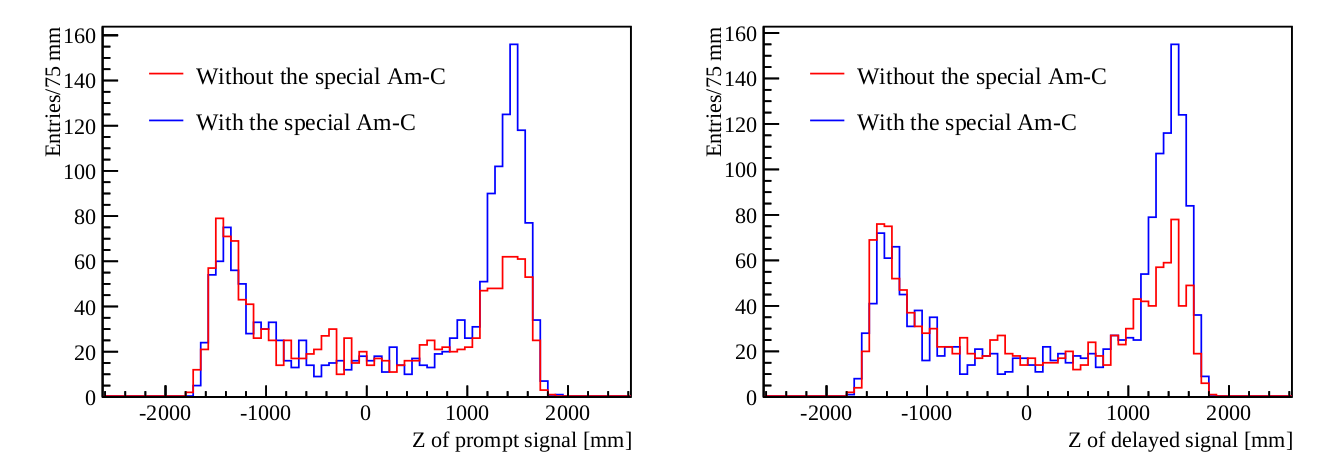
\includegraphics[width=\textwidth]{ch_event_selection/amc_position_asymmetry}
    \caption[Intense \amc{} run vertical positions]{
        Distributions of the reconstructed vertical ($z$) position
        of prompt (left) and delayed (right) signals of nH IBD candidates
        during the special \amc{} run period.
        The red line is from EH3-AD1, which did not have the special \amc{} source,
        and the blue line is from EH3-AD2, which did have the special \amc{} source.
        Figure and caption taken from \cite{nh2016technote}.
    }
    \label{fig:amc_position}
\end{figure}

A modified event selection requiring $z_\text{rec} > 0$
for both prompt and delayed events
was applied to both EH3-AD1 and EH3-AD2 data,
and the accidental background was subtracted.
(The accidental background increased in EH3-AD2 due to additional singles
from the intense \amc{} source.)
By subtracting the prompt energy distribution for EH3-AD1 from that of EH3-AD2,
(see \cref{fig:amc_spectrum}, left)
the number of additional \amc{}-induced events during the intense run
was determined to be
\begin{equation}\label{eq:amc_intense}
    N_\text{int} = N_\text{EH3-AD2}(z > 0) - N_\text{EH3-AD1}(z > 0)
    = \num{121.86\pm41.89}.
\end{equation}
The reconstructed prompt energy spectrum, shown in \cref{fig:amc_spectrum},
was modeled by an exponential function,
\begin{equation}\label{eq:amc_spec_fit}
    f(E; N, E_0) = N e^{-E/E_0}.
\end{equation}
The best-fit values were
\begin{align}\label{eq:amc_spec_params}
    \begin{split}
        N &= 139\pm40 \\
        E_0 &= \SI{0.92\pm0.34}{\MeV}.
    \end{split}
\end{align}
The fit parameter $N$ and the observed count $N_\text{int}$
were highly consistent.

\begin{figure}
    \centering
    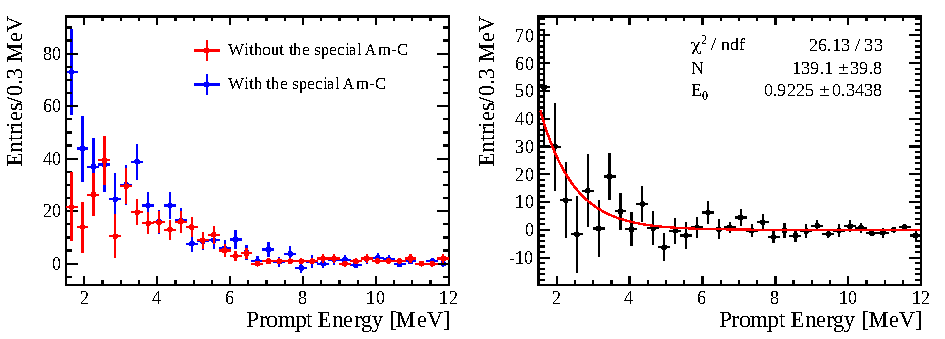
\includegraphics{ch_event_selection/amc_spectrum}
    \caption[\amc{} prompt spectrum]{
        Left: Prompt reconstructed energy spectrum
        for the intense \amc{} source run in EH3-AD2 (blue)
        and for the normal configuration in EH3-AD1 (red).
        Right: Difference between normal and intense prompt spectra,
        fitted by an exponential function, $Ne^{E/E_0}$.
        Figure taken from \cite{nh2016technote}.
    }
    \label{fig:amc_spectrum}
\end{figure}

The measurement from the intense-source run was converted
into rates for each AD during the full data taking period
by computing a proportionality constant
relating the additional singles in the top half of an AD
(relative to the bottom half)
to the rate of \amc{} background events.
Specifically, the number of single events
with energy between \SIlist{6;12}{\MeV} was used
since the impact of the \amc{} source was larger in that range.
The proportionality constant was defined as
\begin{align}\label{eq:amc_proportion}
    \begin{split}
        \alpha_\text{AmC} &= \frac{N_\text{int}}{
            (N_\text{singles, int}(z>0) - N_\text{singles, int}(z < 0))
        }_
        {
            \SI{6}{\MeV} < E < \SI{12}{\MeV}
        } \\
        &= \frac{N_\text{int}}{N_\text{diff, int}}.
    \end{split}
\end{align}
The quantity $N_\text{diff}^{\text{AD }i}$ is defined for each AD $i$
by the same singles asymmetry measurement
given by the denominator of the first line of \cref{eq:amc_proportion}.
The estimated number of \amc{} background events
in the full nominal data sample for AD $i$ is
\begin{equation}\label{eq:amc_count}
    N_\text{AmC}^{\text{AD }i} = \alpha_\text{AmC} N_\text{diff}^{\text{AD }i}.
\end{equation}
A conservative uncertainty in the rate of \SI{50}{\percent}
was sufficient to cover the differences between the observed data
and a variety of simulations of the \amc{} background process.

\subsection{Radiogenic neutron background}
\label{subsec:radn}

The materials used to construct the ADs were
assayed to ensure they emitted only minimal levels of natural radioactivity
\cite{sidebyside}.
However, some residual radioactivity was present,
with dominant contributions from the borosilicate glass comprising the PMT apertures
and the fluorocarbon paint \cite{fluorocarbon_paint} used on the inside of the SSV
to improve the detector uniformity.
Two mechanisms were uncovered which led to a correlated background
due to radiogenic neutrons\cite{rad_n_intro}.
The first was spontaneous fission of \isotope[238]{U},
which could release $\gamma$-rays and/or an energetic neutron,
creating a prompt signal.
Additional neutrons or the same energetic neutron
could subsequently thermalize and capture on Gd or H,
causing the correlated delayed signal.
The second mechanism was the $\text{X}(\alpha, n)\text{Y}$ reaction,
where an $\alpha$ particle emitted from the decay of
either \isotope[238]{U} or \isotope[232]{Th}
would capture on a nearby nucleus
and release an energetic neutron and also potentially a prompt $\gamma$-ray.
The neutron would thermalize and capture on Gd or H, providing a delayed signal.
\Cref{tab:rad_n_sources} lists the \isotope[238]{U} and \isotope[232]{Th}
contaminations of the PMT glass and fluorocarbon paint,
the relevant target nuclei for the $(\alpha,n)$ interaction,
and the estimated rates of neutrons emitted per AD per day.


\ctable[
cap = Radiogenic neutron sources,
caption = {
    Radiogenic neutron sources, broken down by isotope and process
    \cite{rad_n_intro}.
    All values are per AD.
},
label = tab:rad_n_sources,
pos = ht
]{lSS}{}{\FL
    & {Borosilicate glass (PMTs)} & {Fluorocarbon paint} \ML
    Mass [\si{kg}] & 150 & 35 \NN
    \isotope[238]{U} [ppb by mass] & 150 & 35\pm15 \NN
    \isotope[232]{Th} [ppb by mass] & 350 & 175\pm25 \NN
    \addlinespace
    \isotope[238]{U} fission neutrons [\si{\per\day}] & 12 & 0.56 \NN
    $(\alpha, n)$ rate [\si{\per\day}] & 700 & 90 \NN
    \addlinespace
    $(\alpha, n)$ targets & \parbox[t]{3cm}{\strut
    \isotope[10]{B}, \isotope[11]{B},\\ \isotope[17]{O}, \isotope[18]{O},\\
    \isotope[29]{Si}, \isotope[39]{Si}
    \strut} &
    {\isotope[19]{F}} \LL
}

The rate of correlated background events due to radiogenic neutrons
was estimated using a detailed full Monte Carlo simulation \cite{rad_n}.
The LS volume provided significant shielding to the inner GdLS volume,
thus the estimated rate of background events involving nGd capture
was negligible (\SI{0.02}{\per\day}).
However, the rate of nH capture backgrounds was \SI{0.2\pm0.1}{\per\day},
with the uncertainty assigned as a systematic uncertainty
due to the Monte Carlo simulation.

The radiogenic neutron background has not been characterized
using directly-observed data
due to the difficulties in isolating a background with such a small rate
in an environment with a much higher rate of neutrons from other sources
such as muon-induced fast neutrons, \li{}/\he{} decays, and of course IBDs.

\section{Event selection summary}
\label{sec:event_selection_summary}

More than \num{2.1e6} \nuebar{} interactions involving nH capture were observed,
including \num{\sim9e5} at each of EH1 and EH2,
and over \num{3e5} at EH3, where high statistics means
a more precise determination of the disappearance effect due to \thetaot{}.
Including irreducible backgrounds, more than \num{2.5e6}
\nuebar{} candidates were observed in the double-coincidence sample.
The background contamination was overwhelmingly due to accidental coincidences,
comprising \SI{10}{\percent} of the \nuebar{} candidates
at the near halls (EH1 and EH2).
and \SI{50}{\percent} of the \nuebar{} candidates at EH3.
A detailed listing of the full data sample is provided in
\cref{tab:summary_event_selection},
including signal and background rates
as well as detector livetime, target mass variations,
and the muon and multiplicity veto efficiencies $\varepsilon_\mu$ and $\varepsilon_m$.

The Daya Bay experiment's near+far layout meant that a relative comparison
between ADs could be used to extract \thetaot{}
without relying on knowledge of the absolute detection efficiency.
Only the relative variation between ADs was required.
The ADs were designed to be identical,
and differences in the detection efficiencies across ADs
were constrained by the studies presented in \cref{sec:efficiencies}.
The components of the detection efficiency uncertainty
are listed in \cref{tab:efficiency_summary}.

\begin{table}[ht]
    \caption[Event selection summary]{
        Summary of the \nuebar{} event selection results.
        The background and IBD rates are adjusted for
        $\varepsilon_\mu$ and $\varepsilon_m$.
        To convert from rates to counts, multiply by
        $T_\text{DAQ}\varepsilon_\mu\varepsilon_m$.
    }
    \label{tab:summary_event_selection}
    \centering
    \tiny
    \setlength{\tabcolsep}{2.5pt}
    \sisetup{
        per-mode=reciprocal
    }
    \begin{tabular}[t]{rrrrrrrrr}  % 1 label and 8 ADs
        \toprule
        & \multicolumn{2}{c}{EH1}
        & \multicolumn{2}{c}{EH2}
        & \multicolumn{4}{c}{EH3} \\
        \cmidrule(l){2-3} \cmidrule(l){4-5} \cmidrule(l){6-9}
        & EH1-AD1&EH1-AD2&EH2-AD1&EH2-AD2&EH3-AD1&EH3-AD2&EH3-AD3&EH3-AD4 \\
\midrule
        $T_{\text{DAQ}}$ [\si{\day}]& 1534.023&1734.799&1738.961&1551.955&1737.511&1737.511&1737.497&1550.001 \\
        $\Delta N_{\text{p}}$ [\%]& 0.00&-0.01&-0.13&-0.19&0.00&-0.01&0.29&-0.10 \\
        $\varepsilon_{\mu}$& 0.6387&0.6355&0.7063&0.7056&0.9660&0.9659&0.9657&0.9661 \\
        $\varepsilon_{m}$& 0.9510&0.9512&0.9515&0.9519&0.9504&0.9493&0.9493&0.9497 \\
        $R_{\mu}$ [\si{\Hz}]& 199.52&199.38&150.02&149.94&15.02&15.03&15.02&14.92 \\
        $R_s$ [\si{\Hz}]& 18.075&17.973&17.571&17.445&17.178&17.556&17.551&17.417 \\
\arrayrulecolor{lightgray}
\midrule
\arrayrulecolor{black}
        $N_{\text{cand}}$& 473697&544450&542197&471847&162005&164187&166372&144752 \\
        $N_{\text{acc}}$& $53207 \pm 54$&$59411 \pm 57$&$61232 \pm 57$&$52498 \pm 53$&$79658 \pm 64$&$82718 \pm 66$&$84643 \pm 67$&$71966 \pm 62$ \\
        $N_{\text{corr}}$& $420490 \pm 690$&$485039 \pm 740$&$480965 \pm 739$&$419349 \pm 689$&$82347 \pm 408$&$81469 \pm 411$&$81729 \pm 413$&$72786 \pm 385$ \\
        $R_{\text{acc}}$ [\si{\per\day}]& $57.11 \pm 0.06$&$56.65 \pm 0.05$&$52.39 \pm 0.05$&$50.36 \pm 0.05$&$49.94 \pm 0.04$&$51.92 \pm 0.04$&$53.14 \pm 0.04$&$50.61 \pm 0.04$ \\
        $R_{\text{Li9}}$ [\si{\per\day}]& $1.79 \pm 0.87$&$1.79 \pm 0.87$&$2.20 \pm 1.00$&$2.20 \pm 1.00$&$0.21 \pm 0.08$&$0.21 \pm 0.08$&$0.21 \pm 0.08$&$0.21 \pm 0.08$ \\
        $R_{\text{FastN}}$ [\si{\per\day}]& $2.29 \pm 0.18$&$2.29 \pm 0.18$&$1.73 \pm 0.23$&$1.73 \pm 0.23$&$0.16 \pm 0.03$&$0.16 \pm 0.03$&$0.16 \pm 0.03$&$0.16 \pm 0.03$ \\
        $R_{\text{AmC}}$ [\si{\per\day}]& $0.04 \pm 0.02$&$0.04 \pm 0.02$&$0.04 \pm 0.02$&$0.03 \pm 0.01$&$0.02 \pm 0.01$&$0.01 \pm 0.01$&$0.01 \pm 0.01$&$0.01 \pm 0.01$ \\
        $R_{\text{RadN}}$ [\si{\per\day}]& $0.20 \pm 0.10$&$0.20 \pm 0.10$&$0.20 \pm 0.10$&$0.20 \pm 0.10$&$0.20 \pm 0.10$&$0.20 \pm 0.10$&$0.20 \pm 0.10$&$0.20 \pm 0.10$ \\
\addlinespace
        $R_{\text{IBD}}$ [\si{\per\day}]& $446.99 \pm 1.16$&$458.19 \pm 1.14$&$407.35 \pm 1.21$&$398.15 \pm 1.22$&$51.04 \pm 0.29$&$50.56 \pm 0.29$&$50.73 \pm 0.29$&$50.60 \pm 0.30$ \\
\bottomrule
    \end{tabular}
\end{table}

\ctable[
cap = Summary of efficiency uncertainties,
caption = Summary of efficiency uncertainties,
label = tab:efficiency_summary,
pos = ht
]{rS}{
    \tnote[a]{
        Prompt energy cut eff. was treated as an effect of the
        relative energy scale uncertainty,
        so was not included in the total AD-uncorrelated uncertainty.
    }
    \tnote[b]{
        The target proton number uncertainty
        was described in \cref{subsec:target_mass}.
    }
}{\FL
    & {Uncertainty (\%)} \ML
    Prompt energy cut eff.\tmark[a] & 0.1 \NN
    Delayed energy cut eff. & 0.2 \NN
    Distance-time (DT) cut eff. & 0.5 \NN
    Target proton number\tmark[b] & 0.37 \NN
    \addlinespace
    Total AD-uncorrelated uncertainty & 0.66 \tabularnewline\bottomrule
}
